\documentclass[letterpaper,12pt]{report}
\usepackage[top=3cm, bottom=2.5cm, left=2cm, right=2cm]{geometry}
\usepackage{fancyhdr}
\usepackage{glossary}
\usepackage{graphicx}
\usepackage{makeidx}
\usepackage{colortbl}
\usepackage{lscape}
\usepackage{array}
\usepackage{color}
\pagestyle{fancy}
\definecolor{custom}{gray}{0.35}
% For appendix API template
\definecolor{codetxt}{rgb}{0,0,1}
\definecolor{errortxt}{rgb}{0.7,0,0}
\definecolor{warntxt}{rgb}{0.9,0.4,0.1}
\definecolor{datetxt}{gray}{0.2}


\lhead{\textcolor{custom}{\nouppercase{\chaptername{} \space \thechapter \space - Section: \rightmark} }}
\chead{}
\rhead{}
\setlength{\headheight}{15pt}
\setlength{\parindent}{1cm}
\setlength{\parskip}{4mm}
\makeglossary
\makeindex


\begin{document}

\title{Design Document\linebreak WebAgenda\linebreak \linebreak 
	\begin{small}\textbf{Project Team:} Daniel Kettle, Daniel Wehr, Mark Hazlett, Noorin Hasan\linebreak
	\textbf{Client:} Deerfoot Inn and Casino, Robin Featherstone\index{Deerfoot Inn and Casino}\linebreak
	\textbf{Instructor:} Pauline Turnbull\end{small}}

\author{}
\maketitle
\tableofcontents
\listoffigures

\part{Preface}\index{Preface}
\chapter{Document Purpose}
\section{Introduction}
\hspace{1cm}This \index{Requirements Documentation}Requirements Documentation is a product of the need to produce a \textbf{System}\index{system} or Entity that helps a business or company perform a job or series of tasks. The document itself contains information that relates to the objectives\space of this system, the problem that this system is designed to solve, and much of the finer details as well as environmental factors that are taken into consideration. This document will attempt to describe in full detail, the who, what, where, when and why of the System\index{system}.
Here is a brief description of the \textbf{Project}\index{Project} this document refers to:
\paragraph*{WHO  }: We are targeting Businesses and Organizations that do not have functional, sophisticated and easily maintainable scheduling systems, but are looking to implement one without the frustrations of overly complex \index{licensing}licensing, cost, and vendor lock-in. In this \index{Project}Project, the \textbf{Deerfoot Inn and Casino}\index{Deerfoot Inn and Casino} are being directly involved to develop a scheduling system\index{system} free of such inconveniences. This is partially achieved by licensing our product under the \index{General Public Licence}\textbf{General Public Licence (GPL)} and creating a product accessible by anyone with a \index{WebBrowser}\textbf{Web Browser}. The license agreement that the System is distributed with will clearly state any deviation from GPL, if applicable, upon installation. Source code\index{source code} will also be shipped with the product so any programmer or business can use and modify the program according to their needs. Code will be clearly documented for readability and to aid in its development. As our client, the \index{Deerfoot Inn and Casino}Deerfoot Inn and Casino is going to be represented by their VP of Operations, Robin Featherstone. The \index{Deerfoot Inn and Casino}Deerfoot Inn and Casino is going to be the main \textbf{testing}\index{testing} and \textbf{deployment}\index{Deployment} focus for the system and will be used to fulfill all their scheduling needs in most if not all their \textbf{department}s\index{Department}.
\pagebreak
\paragraph{WHAT }: This document describes the Scheduling System\index{system} \index{WebAgenda}"\textbf{WebAgenda}" ©, designed to monitor the schedules of small-to-medium businesses and provide a cheap, easy-to-install-and-use system for scheduling employees. We will be designing it to easily and effectively manage approximately 500 employees for one company. This system does not monitor any other WebAgenda or scheduling systems that may exist on another network, or even on another \textbf{server}\index{server} in the same business or company. Functionality, however, can be built in as users of this software are free to modify it so. This independence may be seen as a security benefit.
\paragraph{WHERE}: As specified above, small-to-medium business are the target and so this system\index{system} is meant to reside on those businesses` servers. In the event that a business does not have a server\index{server}, any computer that runs a server and is connected to the \index{Internet}Internet should theoretically be able to run this software. Any computer with a web browser installed should be able to use the system. In fact, most of the standard browsers will be involved in the testing\index{testing} of the final product that this document describes.
\paragraph{WHEN }: This project\index{project} should be completed in less than six months. Documentation will be released over that period of time along with revisions of this design document. Once complete, the final product will be supported as long as there are people interested or paid to support it. \index{source code}\textbf{Source code} will be freely available if a fix is needed, and as the project developers we may decide to support this product, depending on how this is implemented it may be for a fee.
\paragraph{WHY  }: The world is always in need of powerful, usable, and free software (both as libre and as gratis), especially in the business and IT sector. Many current scheduling solutions have a high cost or limited functionality unless until you purchase the full version. Most, if not all currently marketed scheduling solutions are proprietary and require monthly fees. If you want added functionality you must purchase additional software with possible monthly fees in order to get the job done. With WebAgenda\index{WebAgenda}, additional functionality can be built in-house, contracted out, or even mutually shared with other companies; there are no limitations and you always get the full version, for free.
\paragraph*{} \hspace{1cm}It is not uncommon for businesses to use Excel spreadsheets, paper, or other resourceful but inefficient means to complete scheduling tasks. \index{security}Security is always an issue. Mass distribution of schedules that are \index{encrypted}\textbf{encrypted} and on a need-to-know basis to hundreds of employees are not always feasable for the employer to put into practice, especially when solutions would cost time and money for little benefit when a simpler centralized system\index{system} does the job. This project\index{project} is a college requirement that is designed to have the biggest benefit-to-cost ratio for the widest distribution of potential users and partners.
\newline
\newline
\hspace*{1.3cm}This project\index{project} aims to fulfill an often-overlooked aspect of business that time is wasted on needlessly without compromising productivity gains from the old system\index{system}.
\pagebreak
\chapter{Document Standards}
\textbf{Document Formatting} \index{Document Formatting}All documents included in the project\index{project} that are physically produced will be created using the following standards below. Web-based documentation does not follow all standards, as many do not apply to an electronic medium.
\paragraph*{}This document adheres to the following standards:
\section{Document Standards List}
\begin{itemize}
 \item Single Sided
 \item Bound
 \item Header:\index{Header} [Chapter Title] - [Sub-Chapter Title] w/ a maximum of two sub-chapters per page, using the latter sub-chapter title if this event occurs. Example: Chapter 2 - Section 2.0 Document Standards. Once the header is located in an Appendix, it will only consist of the word ``Appendix'' and the letter that represents that specific appendix.\newline
 \textcolor{custom}{Font should be a shade of grey.}
 \item Footer:\index{Footer} Page number will be:
	\begin{enumerate}
	\item at the bottom center for single-sided pages or
	\item on the outside (bottom left for left-side page, bottom right for right-side page) if document is double-sided
	\end{enumerate}
 \item Images, Pictures, Charts must have figure text below the image, centered beneath it.
	If the figure is less than 40\% of the page width, it can have text wrapped around the \index{figure}figure.
	The figure should always be on the left-hand side of the text if text wrapping exists. 
	If figure is greater than 40\%, it should be on its own lines with no text wrapping it.
 \item All paragraphs will start with a tab of 1 cm in length. The document is generated by \index{Latex}\textbf{Latex} so that there is consistency in these measurements.
 \item Parts, Chapters and Sections are labelled in the Table of Contents due to the importance of their content. Smaller pieces of the document such as subsections and paragraphs, are not.
 \item Any bolded words in the document will have a definition in the glossary except for the beginning of paragraphs, numbers in lists, and titles. For glossary definitions, the bolding only applies to the first instance of the word(s) in the document although multiple instances of a word can still be found in the index.
\end{itemize}

% Must review this paragraph and make changes to wording if it is found unsuitable.

\part{User Requirements}\index{User Requirements}

\chapter{Business Overviews and Objectives}\index{Business Overviews and Objectives}
\hspace{1cm}The Deerfoot Inn and Casino\index{Deerfoot Inn and Casino} is a Canadian-owned casino, hotel and conference center located in Calgary, Alberta. The Deerfoot Inn and Casino is Calgary`s premier hotel and convention center in the southeast quadrant. They provide a large number of entertainment, conference, and meeting areas to accommodate any group and size. With numerous events and conferences every month, the number of clients that the Deerfoot Inn and Casino need to accommodate is immense. They employ a lot of staff to deal with the large workload, but as the workload changes, so does the number of scheduled staff required.
The business objective of the Deerfoot Inn and Casino is to become one of the top casinos in Alberta and to increase profits year after year. They achieve this by sponsoring events, advertising and other marketing means to increase sales, customers, and word-of-mouth.
\pagebreak

\section{Statement of the Problem}\index{Statement of the Problem}
%Put in usage reports -- feature that allows authority to view user's use of the system
\hspace{1cm}\index{Deerfoot Inn and Casino} The Deerfoot Inn and Casino currently schedules their employees by using spreadsheets and paper postings. Creating \index{schedules} based on a paper-based system\index{system} has led to organizational issues and misunderstandings with those who do the scheduling. As the schedules are paper copies posted in common areas, they can get misplaced, damaged (ripped), or removed. In order to change a schedule in circulation, there would have to be a photocopy or an update to the original schedule which could then be printed and distributed. All old copies would have be removed and there would be a risk of employees misinterpreting shifts, employees not showing up, and discontent. When employees do not work consistently for a period of time (2 weeks straight, for example), checking a schedule that can only be read at the workplace can frustrate staff into making assumptions when they work. If a shift change is completed over a paper based scheduling system\index{system}, the supervisor is told of the exchange and a note may be written down on the schedule. A note can be modified or forged by an employee, or the specifics of a shift negotiated after an agreement is made. Misunderstandings could lead to supervisor and management frustration, employees showing up for incorrect times or shifts, and having employees that have not worked being paid for another`s time.
\paragraph{}\hspace{0.6cm}Communicating schedules between departments\index{Department} becomes a difficult task when using a paper-based system\index{system}. If an employee works in multiple departments then having proper communication channels is a neccessity and requires extra work for both supervisors. To schedule shifts for employees that work in multiple departments, one supervisor may have to physically ask another for the current schedule of an employee or by ask via email which would take longer. Every change to the multi-department employee's shifts would have to be communciated to all corresponding supervisors. The frustration could result in affected employees getting less hours, miscommunications for shift details, working two shifts simultaneously, or high employee turnover rate in a worst-case scenario.
\paragraph{}\hspace{0.6cm}One of the problems that arise in the paper-based system that our client has addressed as a priority, is that supervisors do not know when and whether employees have seen the schedule. Even if a schedule has been posted where employees have had ample time to view it, they cannot be sure; likewise, employees may not always been a position to check it until the timeframe becomes short and urgent. With an electronic scheduling system\index{system}, supervisors can send out priority notifications that pop up everytime a user logs in, or while they are using the system. Likewise, employees can check their schedules from virtually anywhere around the globe. One of the features being promoted to the client, is the ability to view when an employee has last logged into the system. This enables supervisors to view trends and follow up on employees that are not checking their schedules for reasons unknown. This function will reduce the number of problem areas for a company.

\section{System Environment}\index{System Environment}
\hspace{1cm}Web Agenda will be hosted on the \index{Deerfoot Inn and Casino}Deerfoot Inn and Casino`s web servers. The scheduling system\index{system} will run alongside their website and function independant of other systems residing on their server\index{server}. It will run on a sub-domain of their current site, allowing the scheduler to be accessed from anywhere at any time provided the user has proper authority to use the service. The system will be able to be accessed through their internal computers as well as any external computer or mobile device with internet access. The system does not deal with monitoring  equipment, daily employee clock-in and clock-out times, or employee payroll information. This is mostly handled by their current system \index{Aloha}Aloha that handles employee payroll information and shift monitoring. The \index{human resources}human resources department\index{Department} relies on the current hourly data from \index{Aloha}Aloha to cover employee wages.

\section{Current System}\index{Current System}
\hspace{1cm}The current scheduling system\index{system} is seen as workable, but lacking. The supervisors and administrators have different methods of scheduling staff under their authority. The schedules are mainly done in a spreadsheet \textbf{format}\index{format} with templates printed and posted on a wall in employee common areas at the hotel or casino. Employees then write down their availability on the posted sheets for that time period. Supervisors and administration use spreadsheets to create official schedules which are then posted back to those areas. However, none of the schedules are identical and therefore become extremely difficult to track employee data. Also, only a limited number of schedules are printed for any given shift period and if they are lost or destroyed for some reason, the supervisor has to go and re-print the schedule to post.
For shift change requests, the employees have to be physically present to complete the transaction. In addition to the validity of the changeover, having both parties present negates the risk of losing the shift change request form or not having it completed properly. There is also the issue of forgeries and miscommunications that the physical presence addresses.

\chapter{System Requirements}\index{System Requirements}
\section{Functional Requirements}\index{Functional Requirements}

Users can export their schedule to a relevant viewer. This allows users to view schedules using different applications assuming the relevant viewer had already been installed. 

\textbf{Document Viewers}
Icons will represent the exporting options. Each icon will hyperlink to display the schedule in the relevant application. The icons displayed will include viewers for:
\begin{enumerate}
 \item MS Word
 \item MS Excel and generic spreadsheets
 \item MS Outlook
 \item Adobe PDF
 \item iCal
 \item iPhone calendar
 \item Android calendar
 \item Blackberry calendar
\end{enumerate}
\pagebreak

We will be designing an \textbf{Information System}\index{Information Systems} to track and plan schedules for staff. The tracking module will include a way for employees to remotely access their schedules, request schedule changes and book days off.

As with any business, the system\index{system} will require the ability to save and retrieve old schedules as well as templates and temporarily saved (partially completed) schedules. They will be stored in a database\index{Database} in this case (as opposed to an excel spreadsheet) which should provide more reliable speed and stability. It`s requirements include having a very very low (non-existant) corruption rate of data. Data validation shall be in place to ensure that the inputs are proper and abide by any constraint it is given. Reliable \textbf{backup}s\index{Backup} are a must and should be completed easily by any staff member who is authorized to do so.

Old schedules should be stored, but not editable, in the database\index{Database}. They should not be saved based on dates because dates on the computer can be changed or modified. While old schedules can be viewed based on their date, they are not defined by it. New schedules that are based on a future date (as opposed to being currently in use) should be editable by appropriate permission users. Only users who are given permissions to edit schedules should be able to edit them. If intervention is required for a current schedule, staff in higher positions of power can be given permissions to make those changes with notifications being sent out to staff that are affected by the change.
\pagebreak
\paragraph*{}\hspace{0.6cm}Staff with default permissions can only view current schedules and request changes. Higher privileged users can edit the current schedule, view older schedules, or make request of higher privileged users. All staff will be able to contact one another through built-in messaging functionality.

The structure of permissions is level-based, with each level having permissions that are equal or greater to the one below. There can be multiple variations of a lower permission level, which can have different levels based off those. Each level has a `root` template: a set of permissions that are the lowest common denominator for that level. A variation of a root template has a suffix that shows that it is a variation.\newline 
\paragraph*{}\hspace{0.6cm} Example: Permission Level 0 is the root and the lowest permission level. Permission Levels 0a, 0b, and 0c have slightly varying and higher permissions which apply to different types of employees. Level 0b can be higher than root level 1, but permission level 1b would have permissions higher than 0b.
\paragraph*{}\hspace{0.6cm}It is possible to elevate permissions from one level to another, provided a higher authority approves of it. Even then, the hightened permissions are temporary.\newline
Common permissions we expect to implement are the following: (see next page)
\pagebreak

\begin{itemize}
 \item Can Read Current Schedule
 \item Can Read Previous Schedules
 \item Can Read Future Schedules (Even though they may be blank)
 \item Can Edit Active Schedule (make changes in real-time)
 \item Can Write Next Schedule
 \item Can Write Future Schedules (This would essentially take employees out of the employee-labour-pool that others could use. Example: Admin wants one employee to serve a specific task that is not a regular task, therefore omitting the employee from a supervisor to schedule him or her to a regular task)
 \item Can View available resources (Employees/Time slots not filled/Report features)
 \item Can Search Previous, Current, or Future Schedules based on criteria specified by the user.
 \item Can change permissions of users [every level of tree is a potential possibility]
 \item Can Read Logs that are generated (What type of logs)
 \item Can create reports [depending on target: previous schedules, all prev schedules, future schedules, or current. Can \textbf{export}\index{export} to other formats.] 
 \item Can export\index{export} schedule to format\index{format} x (current, possibly future depending on restriction)
 \item Can request days off (to what length of time in the future, how many per time slice)
 \item Can request vacation (unlike days off, full-time employees may have extra scheduling benefits)
 \item Can request emergency notifications to supervisors / admin: if in accident, family member dies, act of God occurs and cannot come to work. Able to utilize `not in advance`, but immediately. Should create a notification of some sort to proper admin`s that monitor emp.) This only applies to online requests, disabling this does not mean they cannot phone in.
 \item Can view Inactive Employees (only levels lower than you, not similar authority employees unless granted from higher levels)
 \item Can work shifts on short notice (\# hours/days from shift start)
 \item Can exchange shifts with other employees working similar jobs
 \item Able to send notifications to [type of employee]
\end{itemize}

Permissions list is not comprehensive and subject to change.

Employees should be able to set their availability through the system\index{system} so that the schedules can be auto-generated in addition to ease of use. Schedules can only be changed so often without admin consent. Auto-scheduling must be able to handle hundred upon hundreds of employees and staff.
Should include \textbf{RSS}\index{RSS} functionality, e-mail notifications, have a notifier when logging in to view schedule, a notification rss feed, schedule to device exporting such as palm and blackberry, and schedule to calendar programs such as mozilla suite, \textbf{Mac OS X iCal}\index{Mac OS X iCal} and \textbf{Microsoft Outlook}.

\paragraph*{}\hspace{0.6cm}
The system\index{system} is going to be able to be easily installed on any \index{Sub Domain}\textbf{Sub Domain}. This meaning that any employer or business that would like to use the system has the ability to easily install it, as long as they have a website capable of running the system. The application will be able to handle any management structure that could come up. As a user of the system with the highest permissions, such as a company owner, they will have the ability to create as many different \index{Permissions}permission levels as they deem fit. This allows any company, no matter how large or small to reap the benefits of web agenda. 

Schedule-by-request feature, where employees can request work on a schedule that is optional (provided by higher-ups in the company, for non-essential work opportunities)
The \index{WebAgenda}WebAgenda © program will be licensed under the \index{General Public Licence}General Public Licence 2 so that the company is free to utilize the software to their purposes. Documentation as well as source code\index{source code} will be available to one and all who download/request it.

\pagebreak

\section{Non-Functional Requirements}\index{Non-Functional Requirements}

\hspace{1cm}The scheduling system\index{system} does not monitor employee attendance or payroll functionality, although a stat holiday pay estimate feature will be implemented at the behest of the \index{Deerfoot Inn and Casino}Deerfoot Inn and Casino Manager. \index{WebAgenda}WebAgenda is purely a scheduling, report generating, reference, and distribution system until functionality is extended at a later date.
Scheduling is done by department\index{Department} or by a specific unit of the company.\pagebreak
\paragraph*{}
\hspace{0.6cm}The \index{Deerfoot Inn and Casino}Deerfoot Inn and Casino needs to provide schedules for a minimum of 500 employees. In a worst-case scenario, the system\index{system} must be able to provide 500 constant connections reliably. At full capacity, the system should be able to respond to a user within 2000 milliseconds of a request to view a schedule. For more intensive tasks such as searching for an employee or group of employees in addition to additional filtering, anywhere from 3000 to 5000 milliseconds maximum is reasonable under full load. While there may be potential for a company to include more than 500 employees, the system is designed for optimal performance at 500 or less. WebAgenda does not guarentee accuracy above that limit. Multiple \index{WebAgenda}WebAgenda scheduling systems can be run in parallel to manage certain departments\index{Department} independantly if one scheduler becomes difficult to manage and the hardware is available. System responsiveness will not be guarenteed if more than one system is running at a time. However, it is assumed the hardware will be powerful enough to reach those statistics in such a situation. If multiple scheduling systems are running, staff in one department\index{Department} will only be able to log into the system that holds their department; WebAgenda currently can not communicate with other WebAgenda systems unless data is explicitly exported and imported from database to database. In large corporations, having one scheduling system\index{system} per department could be effective, provided higher management has access to information they need and maintenance support is available; either in the form of official, paid support or staff / IT department.
\paragraph*{}\hspace{0.6cm}
It is up to the supervisors, departments\index{Department}, and administrators to ensure that the schedule is indeed accurate and to their liking. They will have the ability to change things as they desire; a generated schedule will not automatically be uploaded and viewable to all. Rather, it will be saved until it is activated. An active schedule can be seen by anyone with schedule read permissions, and will be seen as official when the schedule`s date coincides with the current date.
The scheduling system\index{system} will also feature a reporting function, which can list employee and schedule data in different ways. This will also be used to test the system for integrity and stability, although it may be restricted to administrators and maintenance staff. The system must have zero tolerance for data loss during operation. This does not account for human error.
\paragraph*{}\hspace{0.6cm}
Most, if not all, of the actions performed on the scheduling system\index{system} are governed by permissions. An employee will have enough permissions to retrieve their schedule, request modifications, book days off within an certain time period from the current date, and change their availability. Depending on the type of employee, permissions may be restricted or granted. A contractor will not be able to book days off or change availability; They can be given an account to remain in contact with the required administration through the messaging system. Supervisors are basically employees with higher  permissions including those that allow them to modify the schedule and to some degree, authorize it. \textbf{Department}\index{Department} leaders, Managers, and administration will have even higher permissions and ultimately be able to approve or modify a supervisor`s decisions in order to suit their needs. Permissions will reflect duty, not overall authority. For maintenance and support of the system, a technician can have access to the system internals while an administrator will have access to creating employees of any type: a permission set that no other employee should have.\pagebreak
\paragraph*{}\hspace{0.6cm}
We will not be selling the software. The system\index{system} also does not monitor anything outside of employees and date-related events; equipment, rooms, and other commonly monitored items are not within the scope of this software. Additional functionality can be built on this software for no cost provided it is licensed similarly. Employee shifts that are scheduled will be measured in time, currently to the nearest quarter of the hour.
Setting up the server\index{server} and performing administrative or \index{server}server-related tasks is in the scope of this project\index{project}, but exists in another document. As the system is running on a \index{server}server, uptime is very important and a backup\index{Backup} server may be of interest to the client. The general consensus for desired server uptime is 99.9\%, which is approximately 364/365 days in the year that the system needs to be accessible. Backing up should not interrupt the function of the server, although restoring a previously backed up database\index{Database} may cause some time for the system to be inaccessible or partially functional.

\newpage
\section{System Interface Requirements}\index{System Interface Requirements}
\hspace{1cm}The employees at the \index{Deerfoot Inn and Casino}Deerfoot Inn and Casino will have varying experience levels using computers. As such, the system\index{system} should be built with a descriptive and intuitive \textbf{interface}. The system will be running as webpage for the front-end, allowing any computer with a web brower and \textbf{javascript}\index{javascript} to interface\index{interface} with it. The employee`s interface should have quick access to their schedule and job-related information with minimal effort. Supervisors and employees with higher permissions should have quick access to functions specific to their job, such as administration. The interface reads and writes information after validating it to the system backend. The backend consists of a database\index{Database} filled with employee and schedule information which can be interpreted by the interface when it is requested by the user. With the addition of a plug-in system, any user of the system can take relevant data from the backend and export\index{export} it to an array of different formats.

Web Agenda is a full web based system\index{system} and therefore in order to get communications out to the employees using the system, it needs to be able to interface\index{interface} with other applications. The following applications need to be able to be communicated with to ensure full functionality and ease of use of the system.
\paragraph*{}\hspace{0.6cm}\textbf{Microsoft Outlook}: This mail application for Microsoft Windows operating system\index{system} is the main mail client that the Deerfoot Inn and Casino\index{Deerfoot Inn and Casino} uses for inter-departmental communication. Our system\index{system} will need to be able to export\index{export} schedules to a format\index{format} that \index{Microsoft Outlook} Microsoft Outlook will be able to import into its calendar function.
\paragraph*{}\hspace{0.6cm}\textbf{Mac OS X ICal}: \index{Mac OS X iCal}This application is an optional application that the application will need to interface\index{interface} with, and may be introduced at a later date as a plug-in as opposed to being added as a full feature upon release. The application needs to be able to export\index{export} calendars and contact information to be added to Mac OS X ICal. Since Mac OS X ICal Is not used directly by the casino but may be used by employee’s using the system\index{system} this will still need to be put into the system at some point.
\paragraph*{}\hspace{0.6cm}\textbf{GNU/Linux KCal}\index{GNU/Linux KCal}: This application is an interface\index{interface} for KOrganizer, one of the more common calendar applications that WebAgenda\index{WebAgenda} will need to communicate with. Kcal is included in one of the two major Linux desktop environments and although it’s not used directly by the Deerfoot Inn and Casino\index{Deerfoot Inn and Casino}, it could still be used by the end user of the system\index{system}. Netbooks and specialized phones may have this software installed.
\newpage

\paragraph*{}\hspace{0.6cm}\textbf{Mobile Web}\index{Mobile Web}: The application will need to be able to work well with mobile devices. That being said the best way to have full functionality across multiple mobile platforms is to have a separate web interface\index{interface} to be able to work well with all mobile web enabled devices. 
Some business tasks are going to be handled by other applications at the Deerfoot Inn and Casino\index{Deerfoot Inn and Casino}. Web Agenda will not need to interface with these applications as they handle aspects of the program that are outside of its scope.
\paragraph*{}\hspace{0.6cm}\textbf{Aloha}\index{Aloha}: Aloha is an employee management system\index{system} that handles tracking when employees clock in and clock out for a shift. This doesn’t handle scheduling of the employees at all. We will not need to interface\index{interface} with Aloha as that would be outside the scope of the project\index{project}.

\paragraph*{}\hspace{0.6cm}
	Our system\index{system} is designed to export\index{export} to calendar formats, spreadsheets, text, and potentially any format the user wants via a plug-in. This generally applies to schedules, although employees with proper permissions can create and output reports. The system will also have to be usable on mobile devices such as phones, personal data assistants, and small laptops. The interface\index{interface} works closely with a permission set that each employee is given. It governs what tasks an employee is able to perform and will display the interface accordingly. The actual WebAgenda\index{WebAgenda} software is distributed with one employee active by default and having all permissions required to allow other users to utilize the system.
\paragraph*{}\hspace{0.6cm}The hardware required to use the system\index{system} are a pointing device, usually a mouse or touch screen depending on what computer is used to access it. A wireless or wired connection to a network that can contact the WebAgenda\index{WebAgenda} server\index{server} is essential. Although not a necessity, having a keyboard or method of character input into the system will be needed to access some of the functionality such as sending messages, editing employee information, and search input. The possibility of using a computer or device without this hardware is almost non-existant as of this document's production.
	

\pagebreak

\section{Maintainability and Administration Requirements}\index{Maintainability and Administration Requirements}
\hspace{1cm}\index{WebAgenda}WebAgenda will be hosted on web servers that are already in service and maintained by the \index{Deerfoot Inn and Casino}Deerfoot Inn and Casino.  IT Staff are already in place for maintaining the hardware for these servers so hardware maintenance will be outside the scope of this project\index{project}.

All employee and scheduling information will be stored in a database\index{Database}.  The WebAgenda\index{WebAgenda} system\index{system} will provide the means for automatic \index{Backup}backups of all data, though selective and manual backup functionality may be introduced at a later date.

	A robust plug-in system\index{system} will be included so that additional functionality can easily be added to the system, such as inclusion of data from Aloha\index{Aloha} or the ability to send notifications through \textbf{SMS}\index{SMS}.  Additional development time will be required to create plug-ins, though the plug-in system should significantly reduce the amount of time that it will take for these features to be created and added compared to more conventional methods.

	Staff may require additional training to review and understand any error messages produced by the system\index{system}, which can then be used to troubleshoot and fix errors.  A knowledgebase will be provided that contains an in-depth explanation of all components of WebAgenda\index{WebAgenda} and its error messages with appropriate solutions.

	At least one manager must be in the system\index{system} with full privileges at all times to act as an administrator over other managers and supervisors.  Without this, certain employees could not have their permissions upgraded; it would not be possible to add new supervisors or managers.

	The previous scheduling system\index{system} must be maintained for at least several months, and will be used in tandem with the WebAgenda\index{WebAgenda} system after it is first brought online.  This will allow for a more comfortable transition between the two systems for all employees, and allow them to fall back on the old system in the event that there are any issues with WebAgenda\index{WebAgenda} during this transition. An emergency plan, in the unlikely event that WebAgenda\index{WebAgenda} should ever fail, will be implemented during the transition.

\pagebreak
\section{Usability Requirements}\index{Usability Requirements}
\hspace{1cm}The system\index{system} needs to be able to be used by a variety of clientelle. Users of the system will vary in experience so the system needs to take this into account. At one end of the spectrum, the system needs to be customizable and intuitive to allow for maximum usability.  On the other end, the system needs to have a lot of functionality and features that advanced users of the system can access upon request without being buried under too many layers.
	With the amount of functionality that the system\index{system} will bring, it`s important that the system is usable by every user to do their jobs. This is a crucial aspect of the system and the interface\index{interface} design of the system that the project\index{project} team will need to keep in mind at every level of the development process.

\part{Requirements Models} \index{Requirements Models}
\chapter{Use Case Diagram}
\index{Use Case Diagram}
\newpage

\begin{figure}[htp]
 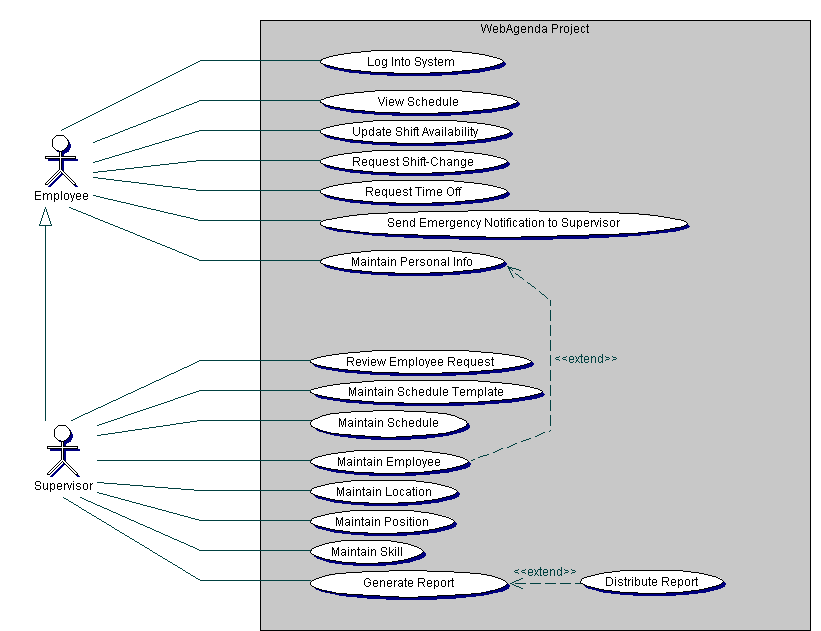
\includegraphics[scale=0.8]{externals/UseCaseDiagram.png}
 \caption{\small
\textbf{\index{WebAgenda}WebAgenda \index{Use Case}Use Case Diagram }\newline A graphical overview of the interactions between users and the system\index{system}.}\label{fig:usecase}

\end{figure}


\chapter{Extended Use Case Diagrams}\index{Extended Use Case Diagrams}
\newcommand{\xuchead}{
		\begin{tabular}{| p{8.5cm} | p{8.5cm} |}
		\hline 
			\cellcolor[gray]{0.8}\textbf{Actor}\index{actor} &\cellcolor[gray]{0.8} \textbf{System}\index{system} \\ 
		\hline
		\end{tabular}
		\newline
		\newline
}

\section{Log-In System}

\begin{description}
 \item \textbf{Description:} \newline The login use case\index{Use Case} goes through how a typical user would log into a \index{system}system. If the user does not enter the correct information they are given an error and they can then re-enter their credentials.
 \item \textbf{Pre Condition:} \newline User must access the online system and have the login page open.
 \item \textbf{Post Condition:} \newline Dashboard is displayed to a newly logged in user
 \item \textbf{Actor:}\index{actor} \newline Employee of a company using WebAgenda\index{WebAgenda}
\end{description}

{
\centering \textbf{Normal Flow}

\begin{center}
\xuchead
% Start another table with information here
\begin{tabular}{| p{8.5cm} | p{8.5cm} |}
\hline
\textbf{1.} User enters a string into the username field of the login screen. & \\
\hline
\textbf{2.} User enters a password into the password field of the login screen. & \\
\hline
\textbf{3.} User presses the ``Log In'' button to log into the system\index{system}. & \\
\hline
\end{tabular}

\end{center}
\pagebreak
% Place onto next page, show header

\xuchead
\begin{tabular}{| p{8.5cm} | p{8.5cm} |}
\hline
& \textbf{4.} System\index{system} takes the value that was entered from the username field and the password field when the log in button was pressed, queries the database\index{Database} and compares the values. \\
\hline
& \textbf{5.} When the values match the values that were queried from the database, proceed to allow access and display the dashboard screen. (A 5.1) \\
\hline
& \textbf{6.} Presents the dashboard screen and populates it with user-specific data. \\
\hline
\end{tabular}



\centering \textbf{Alternate Path 5.1} \linebreak
User enters data into the fields that do not match the database\index{Database} records. 

\begin{center}
\xuchead
\begin{tabular}{| p{8.5cm} | p{8.5cm} |}
\hline
& \textbf{5.1.1} System\index{system} queries the data entered by the user and they do not match the data found in the database. \\
\hline
& \textbf{5.1.2} System displays error message above the username field advising the user that the username/password combination was invalid. \\
\hline
\textbf{5.1.3} User enters data in username field again & \\
\hline
\textbf{5.1.4} User enters data in the password field again & \\
\hline
& \textbf{5.1.5} Return to Normal Flow Step 5. \\
\hline
\end{tabular}
\end{center}
\pagebreak
}
% Start another Extended Use Case
\section{Access Schedule}

\begin{description}
 \item \textbf{Description:} \newline This use case\index{Use Case} will be used for the \index{actor}actor’s accessing their schedule through the schedule screen.
 \item \textbf{Pre Condition:} \newline A user needs to successfully be logged into the system\index{system} and the dashboard screen being displayed.
 \item \textbf{Post Condition:} \newline A schedule widget is displayed to the user with user specific information
 \item \textbf{Actor:} \newline Employee of a company using WebAgenda\index{WebAgenda}
\end{description}

{ \centering \textbf{Normal Flow}
\begin{center}
\xuchead
\begin{tabular}{| p{8.5cm} | p{8.5cm} |}
\hline
\textbf{1.} User clicks on the Users tab & \\
\hline
\textbf{2.} User clicks on Current Schedule link \textit{Note to Mark: changed from schedule button} & \\
\hline
& \textbf{3.} System\index{system} accesses schedule data based on what user is logged in and accessing the schedule screen. (A 3.1) \\ 
\hline
& \textbf{4.} System displays the schedule screen. \\
\hline
& \textbf{5.} System retrieves the schedule widget and displays it on the schedule screen with information specific to the user that is currently logged in. \\
\hline
\end{tabular}
\end{center}
\centering \textbf{Alternate Path 3.1 }
\linebreak User is not added to any current schedule
\begin{center}
\xuchead
\begin{tabular}{| p{8.5cm} | p{8.5cm} |}
\hline
& \textbf{3.1.1} System\index{system} does not pull any schedule data for the current user meaning they are not currently added to any schedule. \\
\hline
& \textbf{3.1.2} System displays a message to the user saying they are not currently scheduled in the system. \\
\hline
\end{tabular}
\end{center}
\pagebreak
}

% A new extended use case
\section{Review Employee Request}
\begin{description}
 \item \textbf{Description:} \newline This use case\index{Use Case} is used for the process of a supervisor reviewing an employee request and either accepting it, deleting it, or updating it.
 \item \textbf{Pre Condition:} \newline The user must be successfully logged into the system\index{system} and on the dashboard screen
 \item \textbf{Post Condition:} \newline A schedule widget is displayed to the user with user specific information
 \item \textbf{Actor:}\index{Actor} \newline An Employee logged into the system with a permission level above other employees in the same job category
\end{description}
{ \centering \textbf{Normal Flow}
\begin{center}
\xuchead
\begin{tabular}{| p{8.5cm} | p{8.5cm} |}
\hline
\textbf{1.} Clicks on the Employee Requests Widget. & \\
\hline
& \textbf{2.} System\index{system} displays the new Employee Requests screen and loads a new copy of the Employee Requests widget. \\
\hline
& \textbf{3.} System loads all the of the requests for that the supervisor that are in the database.\index{Database} \\
\hline
\textbf{4. Loop:} For Each Request - User chooses to approve the request (A 4.1, A 4.2) & \\
\hline
& \textbf{5.} System accepts the change and modifies data in the system based on what type of request was approved. (Example: shift change modifies the shift, etc.) \\
\hline
& \textbf{6.} Notification is sent using the notification in the \index{API}API to however many users are involved in the request. \\
\hline
& \textbf{7.} Removes the request that was approved \\
\hline
\textbf{8. End Loop} & \\
\hline
\end{tabular}
\end{center}
\pagebreak
\centering \textbf{Alternate Path 4.1}
\linebreak User chooses to modify the request
\begin{center}
\xuchead
\begin{tabular}{| p{8.5cm} | p{8.5cm} |}
\hline
\textbf{4.1.1} User clicks the Modify button on the Employee Request widget & \\
\hline
& \textbf{4.1.2} System\index{system} displays text boxes in place of all fields to allow the supervisor to modify values. \\
\hline
\textbf{4.1.3} User Clicks the Submit button to submit the new values (A 4.1.3.1) & \\
\hline
& \textbf{4.1.4} System will accept the new values and change the values in the database\index{Database} according to the new values entered. (E1) \\
\hline
& \textbf{4.1.5} Return to Normal Flow Step 6 \\
\hline
\end{tabular}
\end{center}

\centering \textbf{Alternate Path 4.1.3}
\linebreak User Clicks the Cancel button to cancel any values entered
\begin{center}
\xuchead
\begin{tabular}{| p{8.5cm} | p{8.5cm} |}
\hline
\textbf{4.1.3.1} Actor\index{actor} Clicks the Cancel button & \\
\hline
& \textbf{4.1.3.2} System\index{system} reverts back to the original request that was sent by the employee \\
\hline
& \textbf{4.1.3.3} Return to Normal Flow Step 4 \\
\hline
\end{tabular}
\end{center}

\centering \textbf{Alternate Path 4.2}
\linebreak User Chooses to delete the request
\begin{center}
\xuchead
\begin{tabular}{| p{8.5cm} | p{8.5cm} |}
\hline
\textbf{4.2.1} \index{actor}Actor Presses the Delete button & \\
\hline
& \textbf{4.2.2} System\index{system} erases the request from the screen, however it will still be stored as a disabled user request in the database\index{Database} to be accessed if need be. \\
\hline
\end{tabular}
\end{center}
\pagebreak
\centering \textbf{Error Flow 1}
\linebreak User Enters invalid data after being request is modified
\begin{center}
\xuchead
\begin{tabular}{| p{8.5cm} | p{8.5cm} |}
\hline
\textbf{1.1} \index{actor}Actor Enters invalid data for the Modify Employee Request. & \\
\hline
& \textbf{1.2} System\index{system} queries database\index{Database} to check data. \\
\hline
& \textbf{1.3} System displays error message pertaining to what fields were entered incorrectly. \\
\hline
\textbf{1.4} User Clicks OK button and enters correct data for missing fields. & \\
\hline
\end{tabular}
\end{center}
\pagebreak
}
% Another Extended Use Case please

\section{Add Supervisor}
\begin{description}
 \item \textbf{Description:} \newline This use case\index{Use Case} is used when promoting an employee to a supervisor position. accepting it, deleting it, or updating it.
 \item \textbf{Pre Condition:} \newline A manager must be logged into the system\index{system} and on the maintain employees screen
 \item \textbf{Post-Condition:} \newline Success message telling the logged in user that the employee’s permissions were successfully changed
 \item \textbf{Actor:}\index{actor} \newline User with Permission Level higher than an employee considered to have supervisor authority
\end{description}
{\centering \textbf{Normal Flow}
\begin{center}
\xuchead
\begin{tabular}{| p{8.5cm} | p{8.5cm} |}
\hline
\textbf{1.} \index{actor}Actor presses the promote button & \\
\hline
& \textbf{2.} System produces a message that asks the user if they are sure they want to promote the user to supervisor. \\
\hline
\textbf{3.} \index{actor}Actor Clicks the Confirm button (A 3.1) & \\
\hline
& \textbf{4.} System\index{system} raises the permission level of the user that is promoted by 1. (A 4.1) \\
\hline
& \textbf{5.} System displays a confirmation box displaying the employee`s current permission level and an overview of their now current permissions. \\
\hline
\end{tabular}
\end{center}
}

{\centering \textbf{Alternate Path 3.1}
\linebreak \index{actor}Actor Clicks the Cancel button
\begin{center}
\xuchead
\begin{tabular}{| p{8.5cm} | p{8.5cm} |}
\hline
\textbf{3.1.1} \index{actor}Actor Clicks the Cancel Button & \\
\hline
& \textbf{3.1.2} Return to Normal Flow Step 1. \\
\hline
\end{tabular}
\end{center}
\pagebreak
\centering \textbf{Alternate Path 4.1}
\linebreak Employee does not have a workgroup
\begin{center}
\xuchead
\begin{tabular}{| p{8.5cm} | p{8.5cm} |}
\hline
& \textbf{4.1.1} \index{actor}Actor is Redirected to the Maintain Employee screen (See Maintain Employee extended use case\index{Use Case})  \\
\hline
\end{tabular}
\end{center}
}
\pagebreak

\section{Booking Emergency Days Off}
\begin{description}
 \item \textbf{Description:} \newline This use case\index{Use Case} describes how a user would go about using the WebAgenda\index{WebAgenda} web interface\index{interface} to send an emergency notification for not coming into work. This case assumes that an emergency has happened and the user is not using the  system\index{system} for another reason.
 \item \textbf{Pre Condition:} \newline The user must be successfully logged into the system, presented the dashboard screen and the permission for sending emergency notifications is enabled
 \item \textbf{Post Condition:} \newline A schedule widget is displayed to the user with user specific information
 \item \textbf{Actor:}\index{actor} \newline An employee for the company that can book off days (which may exclude contracting positions)
\end{description}
{ \centering \textbf{Normal Flow}
\begin{center}
\xuchead
\begin{tabular}{| p{8.5cm} | p{8.5cm} |}
\hline
\textbf{1.} Click the ``Users'' tab on the dashboard & \\
\hline
\textbf{2.} Click the ``Days Off'' item on the sidebar & \\
\hline
\textbf{3.} Click on the ``Emergency'' sub-item on the sidebar & \\
\hline
\textbf{4.} Click the ``Next Shift'' radio button option to affect the employee`s next working shift. If the shift has already started, that shift will be the one that is booked off. (A 4.1, A 4.2) & \\
\hline
& \textbf{5.} Present user with an overview of the date(s) booked off and a textbox for them to fill in an optional reason for their absence. \\
\hline
\textbf{6.} User clicks the ``Confirm'' button.& \\
\hline
& \textbf{7.} Send a notification to the user`s supervisor, including the reason for the absence if user entered any text into the textbox. \\
\hline

\end{tabular}
\end{center}


\pagebreak
% Emergency alternate flows
\centering \textbf{Alternate Path 4.1}
\linebreak Book off an extended period of time
\begin{center}
\xuchead
\begin{tabular}{| p{8.5cm} | p{8.5cm} |}
\hline
\textbf{4.1.1.} Click on the extended period radio button  & \\
\hline
\textbf{4.1.2.} User types a number that represents a period that they will be unscheduleable for work. Maximum will be determined by the system\index{system} permissions set. (E 1) & \\
\hline
\textbf{4.1.3.} Clicks Confirm button & \\
\hline
& \textbf{4.1.4.} System\index{system} changes notification message to supervisor including the number of days the employee expects to be away. \\
\hline
\end{tabular}
\end{center}

\centering \textbf{Alternate Path 4.2}
\linebreak Book off an unknown period of time
\begin{center}
\xuchead
\begin{tabular}{| p{8.5cm} | p{8.5cm} |}
\hline
\textbf{4.2.1.} Click on the unknown period radio button  & \\
\hline
\textbf{4.2.2.} Clicks Confirm button & \\
\hline
& \textbf{4.1.3.} System\index{system} changes notification message to supervisor requesting that they contact the employee to understand the situation as the employee may be gone for an unspecified length of time. \\
\hline
\end{tabular}
\end{center}

\centering \textbf{Error Path 4.1.2.}
\linebreak A non-number is entered into the extended period of days to book off field
\begin{center}
\xuchead
\begin{tabular}{| p{8.5cm} | p{8.5cm} |}
\hline
& \textbf{4.1.2.1} Characters that are not numbers will just not appear in the field. \\
\hline
\end{tabular}
\end{center}

}

\pagebreak
\section{Update User Availability}
\begin{description}
 \item \textbf{Description:} \newline An employee that wants to change the days they work has the option to configure a template schedule populated with shifts they can work, called an availability. As long as the template schedule meets minimum shift and hour requirements, within a period of time, they will be able to work that new schedule at their job. Note that the shifts placed in the template are not guarenteed, but schedule creators will have the option of using those employees at those times.
 \item \textbf{Pre Condition:} \newline The user must be successfully logged into the system\index{system}, presented the dashboard screen and the permission for changing availability is enabled
 \item \textbf{Post Condition:} \newline Supervisor does not reject the new availability user creates, duration for availability to take effect passes and new schedule after that date will contain the new availability. Old availability will be archived, current employee availability will be overwritten by new one.
 \item \textbf{Actor:}\index{actor} \newline An employee for the company that is in a position to fill out their availability (contractors may not be able to)
\end{description}
{ \centering \textbf{Normal Flow}
\begin{center}
\xuchead
\begin{tabular}{| p{8.5cm} | p{8.5cm} |}
\hline
\textbf{1.} User clicks on the ``Users'' tab on the dashboard. & \\
\hline
\textbf{2.} User clicks on the Availability link in the sidebar. & \\
\hline
& \textbf{3.} A blank week-long schedule template is produced and presented to the user. A Finish or Complete button will be shown but disabled until a time that the schedule meets requirements. \\
\hline
& \textbf{4.} Weekly Schedule option is selected by default (A 4.1) \\
\hline
\end{tabular}
\end{center}
\pagebreak

\begin{center}
\xuchead
\begin{tabular}{| p{8.5cm} | p{8.5cm} |}
\hline
\textbf{LOOP} & \\
\hline
\textbf{5.} User clicks on one of the 7 columns for each day of the week. Columns are divided up into rows that represent time. Clicking on a row will create a shift object starting at the time representation of the row. & \\
\hline
\textbf{6.} [Optional] User can expand or shrink the shift anywhere in the day by grabbing the start or end row of the shift object and dragging it to another row. User can move an entire shift without resizing it by clicking the middle and dragging it, even between different days. & \\
\hline
\textbf{7.} User creates shifts until the minimum number of shifts (as defined in the system\index{system} permission set) is met and/or until the required number of hours is met. & \\
\hline
\textbf{END LOOP} & \\
\hline
\textbf{8.} User clicks on ``Complete'' button. (A8.1) & \\
\hline
& \textbf{9.} Availability is saved alongside their current availability, which can be blank if they are new. \\
\hline
\textbf{10.} [Optional] User clicks on ``Activate Availability'' button to request that the current user`s availibility be changed to the
saved one. & \\
\hline
& \textbf{11.} Supervisor of the employee is notified that a new availability was filled out. \\
\hline
\end{tabular}
\end{center}

\pagebreak
\centering \textbf{Alternate Path 4.1}
\linebreak Monthly Schedule is selected
\begin{center}
\xuchead
\begin{tabular}{| p{8.5cm} | p{8.5cm} |}
\hline
\textbf{LOOP} & \\
\hline
\textbf{4.1.1.} Continue Normal Flow steps 5 through 7. Once step 7 is finished, user clicks on a button with an arrow icon at the top right of the schedule, another blank template will appear for the user to fill out. & \\
\hline
& \textbf{4.1.2.} Once all the shifts that can be added for the schedule to be valid are added (minimum for all 4 weeks in a month), Activate Schedule button becomes enabled.\\
\hline
& \textbf{4.1.3.} Continue from Normal Flow, Step 8 \\
\hline
\end{tabular}
\end{center}

\centering \textbf{Alternate Path 8.1}
\linebreak User clicks on Clear button
\begin{center}
\xuchead
\begin{tabular}{| p{8.5cm} | p{8.5cm} |}
\hline
\textbf{LOOP} & \\
\hline
& \textbf{8.1.1.} System\index{system} removes all shifts from any applicable weeks that have been edited. \\
\hline
& \textbf{8.1.2.} Presents user with notifications saying that the available template has been cleared. \\
\hline
& \textbf{8.1.3.} Continue from Normal Flow, Step 3. \\
\hline
\end{tabular}
\end{center}

}

\pagebreak
\section{Manager Viewing All Schedules}
\begin{description}
 \item \textbf{Description:} \newline The managers may want a snapshot of all the schedules that are being created / produced within a certain month, as well as quickly accessable links to any period of schedules from the current time forward.
A manager being anyone with a specific level of permissions.
 \item \textbf{Pre Condition:} \newline The user must be successfully logged into the system\index{system}, presented the dashboard screen and is at a permission level where User can read current and future schedules and has employees that can create schedules under their level. User must have a permission level greater than 0 at a minimum.
 \item \textbf{Actor:}\index{actor} \newline An employee for the company that may need confirmation, access to, or a general overview of the business` scheduling specifics
\end{description}
{ \centering \textbf{Normal Flow}
\begin{center}
\xuchead
\begin{tabular}{| p{8.5cm} | p{8.5cm} |}
\hline
\textbf{1.} User clicks on the Administration tab. & \\
\hline
\textbf{2.} Click the View Schedules button & \\
\hline
& \textbf{3.} System\index{system} checks the User`s permission level and fetches all of the  employees with a lower level than User. \\
\hline
& \textbf{4.} A clickable miniature representation image of the schedule is shown on the page in a grid for each employee found in Step 3 for the current date in a widget. \\
\hline
\textbf{5.} User views the schedule representations they want to examine. (A 5.1, A 5.2) & \\
\hline

\end{tabular}
\end{center}
\pagebreak

\begin{center}
\xuchead
\begin{tabular}{| p{8.5cm} | p{8.5cm} |}
\hline
& \textbf{6.} If the User wants to view a schedule in greater detail, they will click on the representation schedule to display it in the widget in full detail, as the creator would view it. \\
\hline
& \textbf{7.} The other schedule representations are moved to a short horizontal widget below the detailed view of the currently viewed schedule. They appear as boxes that have tooltips when the mouse is hovered over them or they are given focus by usually pressing the Tab key. \\
\hline
& \textbf{8.} [Optional] Clicking on a schedule representation in the smaller widget below the schedule displaying widget will swap the currently viewed schedule with the clicked-on schedule, so the selected schedule will be viewed in full detail. \\
\hline
\end{tabular}
\end{center}

\centering \textbf{Alternate Path 5.1}
\linebreak Different Date is selected to view
\begin{center}
\xuchead
\begin{tabular}{| p{8.5cm} | p{8.5cm} |}
\hline
\textbf{5.1.1.} User clicks the Next arrow located above and to the right of the main schedule display widget to view the next month of schedules. & \\
\hline
& \textbf{5.1.2.} New schedule representation images are displayed and the old ones are removed from the widget. \\
\hline
\end{tabular}
\end{center}
\pagebreak

\centering \textbf{Alternate Path 5.2}
\linebreak Different Date is selected to view
\begin{center}
\xuchead
\begin{tabular}{| p{8.5cm} | p{8.5cm} |}
\hline
\textbf{5.2.1.} User clicks the Month Drop Down Menu and selects a month. & \\
\hline
\textbf{5.2.2.} User types in a year to display. (E1, E2) & \\
\hline
& \textbf{5.2.3.} New schedule representation images are displayed and the old ones are removed from the widget. \\
\hline
\end{tabular}
\end{center}

\centering \textbf{Error Path 1}
\linebreak Number is not entered into the year text field
\begin{center}
\xuchead
\begin{tabular}{| p{8.5cm} | p{8.5cm} |}
\hline
& \textbf{1.1} Any non-number detected input will be ignored. \\
\hline
\end{tabular}
\end{center}

\centering \textbf{Error Path 2}
\linebreak No schedules are found for the year entered
\begin{center}
\xuchead
\begin{tabular}{| p{8.5cm} | p{8.5cm} |}
\hline
& \textbf{2.1} No schedule representation images are displayed. Text is displayed stating that no schedules exist for that year while displaying the current year. \\
\hline 
\end{tabular}
\end{center}

}

\pagebreak
\section{Book Days Off}
\begin{description}
 \item \textbf{Description:} \newline How an employee should go about booking days off in advance. Unlike emergency requests which is to accomidate rare and difficult circumstances, this requires a supervisor`s permission level or greater to be granted or denied. There are a pre-defined number of days, weeks, or time periods that can be booked off.
 \item \textbf{Pre Condition:} \newline The user must be successfully logged into the system\index{system}, presented the dashboard screen and have permissions to book days off. The user must also have a supervisor for this to have any effect. Schedules cannot be accessed previous to the current date plus the buffer period for requesting days off as specified by the system permission set.
 \item \textbf{Post Condition:} \newline Schedules are modified, supervisor is notified.
 \item \textbf{Actor:} \index{actor}\newline Employee who logs into the system can have any permission set as long as they have a supervisor to approve of the request.
\end{description}
{ \centering \textbf{Normal Flow}
\begin{center}
\xuchead
\begin{tabular}{| p{8.5cm} | p{8.5cm} |}
\hline
\textbf{1.} Click the ``Users'' tab on the dashboard. & \\
\hline
\textbf{2.} Click the ``Days Off'' item on the sidebar. & \\
\hline
& \textbf{3.} Displays the number of days off that the user can take (There is a limit imposed every year-month- or week) and a schedule starting at the next available day to book off (as specified by system\index{system}, defaulted to 2 week wait if not set). \\
\hline
\end{tabular}
\end{center}
\pagebreak

\begin{center}
\xuchead
\begin{tabular}{| p{8.5cm} | p{8.5cm} |}
\hline
\textbf{4.} Selects a period of time by clicking on a day object in the schedule for the number of times the day off counter is above 0. Clicking on a day that is already selected will deselect it and add back to the day off counter. No partial days can be booked off. If the user wants to work a partial day, they will have to ask a supervisor to edit their current schedule to accompany the request. \\
\hline
& \textbf{5.} For every booked off day, a day off counter is removed ( -1 ) (A 5.1) \\
\hline
\textbf{6.} User clicks the Confirm button. (A 6.1) & \\
\hline
& \textbf{7.} Is shown details of selection (in a list) of days booked off and asked to confirm again. (A 6.1) \\
\hline
& \textbf{8.} System\index{system} notifies supervisor of the book off requests (A 8.1) and supervisor accepts the request. \\
\hline
& \textbf{9.} Schedule is modified. \\
\hline
\end{tabular}
\end{center}

% NEed to do alternatives
\centering \textbf{Alternate Path 5.1}
\linebreak No counters, no more days off to book
\begin{center}
\xuchead
\begin{tabular}{| p{8.5cm} | p{8.5cm} |}
\hline
\textbf{5.1.1.} Clicks on a day off when counter is at 0 & \\
\hline
& \textbf{5.1.2.} Nothing happens. \\
\hline
\end{tabular}
\end{center}


\centering \textbf{Alternate Path 6.1}
\linebreak Clear off booked days
\begin{center}
\xuchead
\begin{tabular}{| p{8.5cm} | p{8.5cm} |}
\hline
\textbf{6.1.1.} Clicks Clear button & \\
\hline
& \textbf{6.1.2.} Any days off are deselected and counters restored for every day.  \\
\hline
\end{tabular}
\end{center}

\pagebreak
\centering \textbf{Alternate Path 8.1}
\linebreak Supervisor rejects the request
\begin{center}
\xuchead
\begin{tabular}{| p{8.5cm} | p{8.5cm} |}
\hline
& \textbf{8.1.1.} Counters are returned to the user, schedule is not modified. \\
\hline
& \textbf{8.1.2.} Notification is sent to user with an optional explination as to why their request was refused. \\
\hline
\end{tabular}
\end{center}

}

\pagebreak
\section{Request Shift Change}
\begin{description}
 \item \textbf{Description:} \newline An employee wants to get rid of a shift, or trade a shift because the shift is at an inconvenient time. Instead of booking the day off, leaving the business short-staffed, or if employee is unable to book it off as the due date is past, they can ask their fellow employees to take the shift instead. A supervisor has permissions to revert the changes if they do not want the changes to take place. The supervisor’s supervisor has the ability to overrule that decision, to keep a reign on lower authority supervisors in case decisions are found to be biased.
 \item \textbf{Pre Condition:} \newline The user must be successfully logged into the system\index{system}, presented the dashboard screen and have permissions to request the shift be taken. Only an employee with the same permission set or higher can accept a request. 
 \item \textbf{Post Condition:} \newline Schedule is updated with the involved employees according to the shift(s) being modified.
 \item \textbf{Actor:}\index{actor} \newline Employee who logs into the system\index{system} has a job they are working. Higher permission set employees may have trouble finding replacements as generally there are less high-position workers in a company than lower-position workers.
\end{description}
{ \centering \textbf{Normal Flow}
\begin{center}
\xuchead
\begin{tabular}{| p{8.5cm} | p{8.5cm} |}
\hline
\textbf{1.} User clicks on the Users tab & \\
\hline
\textbf{2.} User clicks on the Request Shift Change link in the sidebar. & \\
\hline
\textbf{3.} User selects one shift from their schedule (shown in a widget) that they want to trade.  & \\
\hline
\textbf{4.} User clicks Confirm. (A 4.1) & \\
\hline
& \textbf{5.} The request for the shift change is placed in the Shift Exchange Pool, a list of all the shifts that employees want to get rid of. \\
\hline
& \textbf{6.} System\index{system} waits for another employee to accept the proposed shift. (A 6.1) \\
\hline
& \textbf{7.} Shift is accepted from another employee, notifications are sent to User’s supervisor (A 7.1) \\
\hline
& \textbf{8.} Schedules of both employees are changed. (A 8.1) \\
\hline
\end{tabular}
\end{center}
\pagebreak

\centering \textbf{Alternate Path 4.1}
\linebreak User requested specific employee to change shifts with.
\begin{center}
\xuchead
\begin{tabular}{| p{8.5cm} | p{8.5cm} |}
\hline
& \textbf{4.1.1.} List is populated of people that have the same job type that User works. \\
\hline
\textbf{4.1.2.} User clicks on an employee name (which is a link) . &  \\
\hline
& \textbf{4.1.3.} Displays information on the request and asks for confirmation. (A 4.1.3.1., A 4.1.4.1.) \\
\hline
\textbf{4.1.4} Clicks Confirm to send request. & \\
\hline
& \textbf{4.1.5.} Looks up employee and sends request to them. \\
\hline
& \textbf{4.1.6.} Notification is sent to supervisor with option to revert the request. \\
\hline
& \textbf{4.1.7.} Resume at Normal Flow Step 8. \\
\hline
\end{tabular}
\end{center}

\centering \textbf{Alternate Path 4.1.3.1.}
\linebreak Cancel pending shift request to employee
\begin{center}
\xuchead
\begin{tabular}{| p{8.5cm} | p{8.5cm} |}
\hline
\textbf{4.1.3.1.1.} Clicks on ``Users'' tab. & \\
\hline
\textbf{4.1.3.1.2.} Clicks on Request Shift Change link in sidebar. & \\
\hline
& \textbf{4.1.3.1.3.} Pending Request in progress will be shown in sidebar below Request Shift Change link. \\
\hline
\textbf{4.1.3.1.4.} Click on Pending Request link. & \\
\hline
& \textbf{4.1.3.1.5.} Displays information on the pending request and a button to drop request. \\
\hline
\textbf{4.1.3.1.6.} Clicks ``Drop Request`` button. & \\
\hline
& \textbf{4.1.3.1.7.} Notification is sent to the employee mentioning that a shift request was cancelled by User. \\
\hline
\end{tabular}
\end{center}

\pagebreak

\centering \textbf{Alternate Path 4.1.4.1.}
\linebreak Employee can work as requested by user
\begin{center}
\xuchead
\begin{tabular}{| p{8.5cm} | p{8.5cm} |}
\hline
& \textbf{4.1.4.1.1.} Requested employee is notified that a shift change request is pending. \\
\hline
\textbf{4.1.4.1.2.} Employee denies request \newline (A 4.1.4.1.2.1.). & \\
\hline
& \textbf{4.1.4.1.3.} Notification is sent back to user explaining request was denied. (A 4.1.4.1.3.1.). \\
\hline
& \textbf{4.1.4.1.4.} System\index{system} removes Pending Request. \\
\hline
\end{tabular}
\end{center}

\centering \textbf{Alternate Path 4.1.4.1.2.1.}
\linebreak Employee accepts request that is sent by User
\begin{center}
\xuchead
\begin{tabular}{| p{8.5cm} | p{8.5cm} |}
\hline
& \textbf{4.1.4.1.2.1.1.} Employee accepts request to take User’s shift. \\
\hline
& \textbf{4.1.4.1.2.1.2.} Notification of acceptance is sent to user. \\
\hline
& \textbf{4.1.4.1.2.1.3.} Schedule of both users are modified accordingly. \\
\hline
\end{tabular}
\end{center}

\centering \textbf{Alternate Path 4.1.4.1.3.1.}
\linebreak Employee silently ignores the request
\begin{center}
\xuchead
\begin{tabular}{| p{8.5cm} | p{8.5cm} |}
\hline
& \textbf{4.1.4.1.3.1.1.} Employee requests to have request ignored. \\
\hline
& \textbf{4.1.4.1.3.1.2.} Shift is seen as pending until time for shift approaches. Unless User cancels the request and gets someone else to work it, they will be expected to work that shift. \\
\hline
\end{tabular}
\end{center}

\pagebreak

\centering \textbf{Alternate Path 6.1.}
\linebreak No user accepts the shift in time (either request pool or specific request) 
\begin{center}
\xuchead
\begin{tabular}{| p{8.5cm} | p{8.5cm} |}
\hline
& \textbf{6.1.1.} Notification is sent to User saying that the shift could not be traded. \\
\hline
& \textbf{6.1.2.} Remove the pending request. \\
\hline
\end{tabular}
\end{center}

\centering \textbf{Alternate Path 7.1.}
\linebreak Employee and User have different supervisors
\begin{center}
\xuchead
\begin{tabular}{| p{8.5cm} | p{8.5cm} |}
\hline
& \textbf{7.1.1.} Notifications are sent to both supervisors. (A 8.1.) \\
\hline
\end{tabular}
\end{center}

\centering \textbf{Alternate Path 8.1.}
\linebreak Supervisor reverts decision to have shift change
\begin{center}
\xuchead
\begin{tabular}{| p{8.5cm} | p{8.5cm} |}
\hline
& \textbf{8.1.1.} Supervisor is notified of the exchange and clicks on the Reverse Decision button. \\
\hline
& \textbf{8.1.2.} Employees that had their schedules modified have changes reverted. \\
\hline
& \textbf{8.1.3.} Notifications are sent to both employees informing them that the schedules are reversed. \\
\hline
& \textbf{8.1.4.} Supervisor has information displayed that encourages them to contact the employees to explain why decision was reversed. \\
\hline
& \textbf{8.1.5.} Notification is sent to supervisor’s supervisor notifying them that a decision was overruled. (A 8.1.5.1.) \\
\hline
\end{tabular}
\end{center}

\pagebreak

\centering \textbf{Alternate Path 8.1.4.1.}
\linebreak Supervisor`s Supervisor reverts the previous decision
\begin{center}
\xuchead
\begin{tabular}{| p{8.5cm} | p{8.5cm} |}
\hline
& \textbf{8.1.4.1.1.} Involved employees are sent a notification that mentions their shifts have been changed yet again. \\
\hline
& \textbf{8.1.4.1.2.} Schedules are changed. \\
\hline
& \textbf{8.1.4.1.3.} Notification is sent back to supervisor explaining that their decision was overturned. \\
\hline
\end{tabular}
\end{center}

}

\pagebreak
\section{Distribute Reports}
\begin{description}
 \item \textbf{Description:} \newline Once a report has been generated, it can be sent to others as an electronic copy through email, or it can be printed and distributed by paper.
 \item \textbf{Pre Condition:} \newline A report has been generated and is displayed on the screen.
 \item \textbf{Post Condition:} \newline  A report has been printed or emailed, and the user has returned to the report view.
 \item \textbf{Actor:}\index{actor} \newline An Employee who has Supervisor permissions.
\end{description}
{ \centering \textbf{Normal Flow}
\begin{center}
\xuchead
\begin{tabular}{| p{8.5cm} | p{8.5cm} |}
\hline
\textbf{1.} User clicks distribute report button. & \\
\hline
& \textbf{2.} System\index{system} displays distribution option list. \\
\hline
\textbf{3.} User clicks the print report link. (A 3.1) & \\
\hline
& \textbf{4.} Generate print-friendly version of the report. \\
\hline
& \textbf{5.} Display report on screen. \\
\hline
& \textbf{6.} Initiate web browser`s print action. \\
\hline
\textbf{7.} Prints report (Browser functions outside project\index{project} scope) & \\
\hline
\textbf{8.} User clicks return to report view link. & \\
\hline
& \textbf{9.} Reload report view. \\
\hline
\end{tabular}
\end{center}
\pagebreak

\centering \textbf{Alternate Path 3.1}
\linebreak E-Mail report link selected
\begin{center}
\xuchead
\begin{tabular}{| p{8.5cm} | p{8.5cm} |}
\hline
& \textbf{3.1.1.} Display email entry field. \\
\hline
\textbf{3.1.2.} User enters e-mail address. & \\
\hline
& \textbf{3.1.3.} System\index{system} verifies that email is in proper format. (E 1)\\
\hline
& \textbf{3.1.4.} Enable Send Emails button. \\
\hline
\textbf{3.1.5.} Press send Emails button. & \\
\hline
& \textbf{3.1.6.} Send report to listed emails. \\
\hline
& \textbf{3.1.7.} Display emails sent successfully. \\
\hline
\textbf{3.1.8.} Clicks OK Button. & \\
\hline
& \textbf{3.1.9.} Use case\index{Use Case} resumes at step 9. \\
\hline
\end{tabular}
\end{center}

\centering \textbf{Error Path 1.1}
\linebreak Entered email(s) detected as invalid
\begin{center}
\xuchead
\begin{tabular}{| p{8.5cm} | p{8.5cm} |}
\hline
& \textbf{1.1.} Highlight invalid emails \\
\hline
& \textbf{1.2.} Request that user corrects or removes invalid emails. \\
\hline
\textbf{1.3.} Correct email addresses. & \\
\hline
& \textbf{1.4.} Use Case\index{Use Case} resumes at Step 3.1.3. \\
\hline
\end{tabular}
\end{center}

}

\pagebreak
\section{Generate Reports}
\begin{description}
 \item \textbf{Description:} \newline Supervisors can generate reports give information on schedules, employees and their usage of the system\index{system}. 

Schedule Reports list information on previously implemented schedules, or future schedules that have yet to take effect.

Employee Resource Reports list information such as employees that are free during a given time, or future timeslots that have yet to be filled. 

Employee Usage Reports will allow supervisors to see statistics on how employees are using the system\index{system}.  This will include information such as when they last viewed their schedule, which will allow supervisors to see who might not yet know about changes that have been made.

 \item \textbf{Pre Condition:} \newline The supervisor has successfully logged in; Dashboard is displayed.
 \item \textbf{Post Condition:} \newline A specific report is displayed, and can be printed or emailed if desired.
 \item \textbf{Actor:}\index{actor} \newline An Employee who has Supervisor permissions.
\end{description}
{ \centering \textbf{Normal Flow}
\begin{center}
\xuchead
\begin{tabular}{| p{8.5cm} | p{8.5cm} |}
\hline
\textbf{1.} User clicks button to enter report view. & \\
\hline
& \textbf{2.} Display front page of report view, listing report types. \\
\hline
\textbf{3.} User selects Schedule Report, enters date range for report. (A 3.1, A 3.2) & \\
\hline
& \textbf{4.} Collect schedule data. \\
\hline
& \textbf{5.} Generate schedule data. \\
\hline
& \textbf{6.} Display report. \\
\hline
\end{tabular}
\end{center}
\pagebreak
\centering \textbf{Alternate Path 3.1}
\linebreak Employee Resource Report selected
\begin{center}
\xuchead
\begin{tabular}{| p{8.5cm} | p{8.5cm} |}
\hline
& \textbf{3.1.1.} Collect employee and employee`s shift data. \\
\hline
& \textbf{3.1.2.} Generate resource report. \\
\hline
& \textbf{3.1.3.} Use case\index{Use Case} continues at Step 6. \\
\hline
\end{tabular}
\end{center}

\centering \textbf{Alternate Path 3.2}
\linebreak E-Mail Employee Usage Report selected
\begin{center}
\xuchead
\begin{tabular}{| p{8.5cm} | p{8.5cm} |}
\hline
& \textbf{3.2.1.} Collect employee and employee`s schedule data. \\
\hline
& \textbf{3.2.2.} Generate usage report. \\
\hline
& \textbf{3.2.3.} Use case\index{Use Case} continues at Step 6. \\
\hline
\end{tabular}
\end{center}

}

\pagebreak
\section{Maintain Workgroups}
\begin{description}
 \item \textbf{Description:} \newline Managers are able to create, edit and delete employee workgroups.  When a new workgroup is created, the manager may choose to assign employees to the workgroup, or leave it empty for employees to be added at a later date.
 \item \textbf{Pre Condition:} \newline  The manager has successfully logged in; Dashboard is displayed.
 \item \textbf{Post Condition:} \newline The manager has finished creating/editing/deleting a workgroup, and has returned to the available workgroups list.
 \item \textbf{Actor:}\index{actor} \newline An Employee who has Manager permissions.
\end{description}
{ \centering \textbf{Normal Flow}
\begin{center}
\xuchead
\begin{tabular}{| p{8.5cm} | p{8.5cm} |}
\hline
\textbf{1.} User clicks the Administration tab. & \\
\hline
\textbf{2.} User clicks maintain workgroups link in sidebar. & \\
\hline
& \textbf{3.} Load maintain workgroups widget. \\
\hline
& \textbf{4.} Populate available workgroups list. \\
\hline
\textbf{5.} Presses create new workgroup button. (A 4.1, A 4.2) & \\
\hline
& \textbf{6.} Creates new workgroup. \\
\hline
& \textbf{7.} Populate available employees list. \\
\hline
& \textbf{8.} Display edit workgroup view. \\
\hline
\textbf{9.} Enters new workgroup name. \\
\hline
\textbf{10.} Selects employees to add to workgroup. & \\
\hline
\textbf{11.}  Clicks add employees to workgroup button. & \\
\hline
& \textbf{12.} Show dialog requesting confirmation and displaying employee info. \\
\hline
\textbf{13.} Clicks accept changes button (A 13.1.) & \\
\hline
& \textbf{14.} Save workgroup. \\
\hline
& \textbf{15.} Return to available workgroups list. \\
\hline
\end{tabular}
\end{center}

\pagebreak

\centering \textbf{Alternate Path 4.1}
\linebreak Manager edits workgroup
\begin{center}
\xuchead
\begin{tabular}{| p{8.5cm} | p{8.5cm} |}
\hline
\textbf{4.1.1.} Selects workgroup from available workgroup list. & \\
\hline
\textbf{4.1.2.} Clicks edit workgroup button. & \\
\hline
& \textbf{4.1.3.} Load selected workgroup. \\
\hline
& \textbf{4.1.4.} Populate available employees list. \\
\hline
\textbf{4.1.5.} Selects employees to add to workgroup. (A 4.1.4.1.) & \\
\hline
\textbf{4.1.6.} Clicks add employees to workgroup button. & \\
\hline
& \textbf{4.1.7.} Use case\index{Use Case} resumes at Step 11. \\
\hline
\end{tabular}
\end{center}

\centering \textbf{Alternate Path 4.1.4.1.}
\linebreak Manager edits workgroup
\begin{center}
\xuchead
\begin{tabular}{| p{8.5cm} | p{8.5cm} |}
\hline
\textbf{4.1.4.1.1.} Clicks remove employees button. & \\
\hline
& \textbf{4.1.4.1.2.} Use case\index{Use Case} resumes from Step 11. \\
\hline
\end{tabular}
\end{center}


\centering \textbf{Alternate Path 4.2.}
\linebreak Manager deletes workgroup
\begin{center}
\xuchead
\begin{tabular}{| p{8.5cm} | p{8.5cm} |}
\hline
\textbf{4.2.1.} Selects workgroup from available workgroup list. & \\
\hline
\textbf{4.2.2.} Clicks delete workgroup button. & \\
\hline
& \textbf{4.2.3.} Use case\index{Use Case} resumes from Step 11. \\
\hline
\end{tabular}
\end{center}

\pagebreak

\centering \textbf{Alternate Path 12.1.}
\linebreak Manager clicks cancel changes button.
\begin{center}
\xuchead
\begin{tabular}{| p{8.5cm} | p{8.5cm} |}
\hline
& \textbf{12.1.1.} Undo changes, deselect employees. \\
\hline
& \textbf{12.1.2.} Use case\index{Use Case} resumes from Step 9. \\
\hline
\end{tabular}
\end{center}

}

\pagebreak
\section{Send Announcement}
\begin{description}
 \item \textbf{Description:} \newline Custom announcements can be created that will be sent to specific employees, employee types, or all employees working under the supervisor.
 \item \textbf{Pre Condition:} \newline The supervisor has successfully logged in; Dashboard is displayed.
 \item \textbf{Post Condition:} \newline The supervisor has finished sending an announcement, and is able to send another or return to the dashboard.
 \item \textbf{Actor:}\index{actor} \newline An Employee who has Supervisor permissions.
\end{description}
{ \centering \textbf{Normal Flow}
\begin{center}
\xuchead
\begin{tabular}{| p{8.5cm} | p{8.5cm} |}
\hline
\textbf{1.} Clicks send announcement button. & \\
\hline
& \textbf{2.} Load announcement widget. \\
\hline
& \textbf{3.} Display announcement type selection view. \\
\hline
\textbf{4.} Presses workgroup announcement button. (A 4.1) & \\
\hline
& \textbf{5.} Populate and display list of workgroups for supervisor. \\
\hline
\textbf{6.} Selects target workgroup from list. & \\
\hline
\textbf{7.} Enters announcement message. & \\
\hline
\textbf{8.} Presses send button. & \\
\hline
& \textbf{9.} Send announcement to all employees within selected workgroup. \\
\hline
& \textbf{10.} Display messages sent alert window. \\
\hline
\textbf{11.} Clicks ok button on alert window. & \\
\hline
& \textbf{12.} Return to announcement type selection view. \\
\hline
\end{tabular}
\end{center}
\pagebreak
\centering \textbf{Alternate Path 4.1.}
\linebreak Presses employee type announcement button
\begin{center}
\xuchead
\begin{tabular}{| p{8.5cm} | p{8.5cm} |}
\hline
& \textbf{4.1.1.} Populate and display list of employee types for supervisor. \\
\hline
\textbf{4.1.2.} Selects target employee type. & \\
\hline
\textbf{4.1.3.} Enters announcement message. & \\
\hline
\textbf{4.1.4.} Presses send button. & \\
\hline
& \textbf{4.1.5.} Send announcement message to all employees within selected employee type. \\
\hline
& \textbf{4.1.6.} Use case\index{Use Case} resumes from Step 9. \\
\hline
\end{tabular}
\end{center}


}

\pagebreak
\section{View Workgroup Schedule}
\begin{description}
 \item \textbf{Description:} \newline After entering the schedule view, supervisors can select to view a schedule for a specific workgroup of employees.  Weekly schedules are displayed by default, which can be switched to a daily schedule if desired.
 \item \textbf{Pre Condition:} \newline The supervisor has successfully logged in; Dashboard is displayed.
 \item \textbf{Post Condition:} \newline The schedule for a specific workgroup is displayed.
 \item \textbf{Actor:}\index{actor} \newline An Employee who has Supervisor permissions.
\end{description}
{ \centering \textbf{Normal Flow}
\begin{center}
\xuchead
\begin{tabular}{| p{8.5cm} | p{8.5cm} |}
\hline
\textbf{1.} Clicks schedules button to enter schedule view. (A 1.1) & \\
\hline
& \textbf{2.} Get schedule data on super workgroup (all employees) for supervisor. \\
\hline
& \textbf{3.} Populate workgroup dropdown list. (E 1) \\
\hline
& \textbf{4.} Display weekly schedule view of super workgroup for current date, listing workgroups in dropdown box. \\
\hline
\textbf{5.} Selects workgroup from dropdown box. & \\
\hline
& \textbf{6.} Reload schedule view, showing employees only from selected workgroup. \\
\hline
& \textbf{7.} Get schedule data for employees in the selected workgroup for the given time period. \\
\hline
& \textbf{8.} Display workgroup schedule. \\
\hline
\end{tabular}
\end{center}

\centering \textbf{Alternate Path 1.1.}
\linebreak Daily schedule selected
\begin{center}
\xuchead
\begin{tabular}{| p{8.5cm} | p{8.5cm} |}
\hline
& \textbf{1.1.1.} Get daily schedule data for employees in seelected workgroup only. \\
\hline
& \textbf{1.1.2.} Use case\index{Use Case} resumes from Step 1. \\
\hline
\end{tabular}
\end{center}
\pagebreak
\centering \textbf{Error Path 1.1.}
\linebreak No additional workgroups exist
\begin{center}
\xuchead
\begin{tabular}{| p{8.5cm} | p{8.5cm} |}
\hline
& \textbf{1.1.1.} Disable workgroup dropdown list. \\
\hline
& \textbf{1.1.2.} Use case\index{Use Case} resumes at Step 4. \\
\hline
\end{tabular}
\end{center}

}


% Maintain Location 

\pagebreak
\section{Maintain Locations}
\begin{description}
 \item \textbf{Description:} \newline Supervisors are able to create, edit and delete locations.  Once created, employees can choose or be assigned a preferred location, used for automated scheduling.
 \item \textbf{Pre Condition:} \newline The manager has successfully logged in; Dashboard is displayed.
 \item \textbf{Post Condition:} \newline The manager has finished creating/editing/deleting a location, and has returned to the dashboard.
 \item \textbf{Actor:}\index{actor} \newline  An Employee who has Supervisor permissions.
\end{description}
{ \centering \textbf{Normal Flow}
\begin{center}
\xuchead
\begin{tabular}{| p{8.5cm} | p{8.5cm} |}
\hline
\textbf{1.} Clicks maintain locations button. & \\
\hline
& \textbf{2.} Load maintain locations widget. \\
\hline
& \textbf{3.} Display location list view, populating location list. \\
\hline
\textbf{4.} Clicks add location button. (A4.1) & \\
\hline
& \textbf{5.} Display empty edit location view. \\
\hline
\textbf{6.} Enters location name and description. & \\
\hline
\textbf{7.} Clicks save button. & \\
\hline
& \textbf{8.} Confirm location does not already exist. (E1) \\
\hline
& \textbf{9.} Save location in database \\
\hline
& \textbf{10.} Display location saved alert. \\
\hline
\textbf{11.} Clicks OK button on alert & \\
\hline
& \textbf{12.} Display location list view, populating location list. \\
\hline
\textbf{13.} Clicks return to dashboard link. & \\
\hline


\end{tabular}
\end{center}
\pagebreak
\centering \textbf{Alternate Path 4.1.}
\linebreak Selects existing location
\begin{center}
\xuchead
\begin{tabular}{| p{8.5cm} | p{8.5cm} |}
\hline
\textbf{4.1.1.} Clicks edit location button. (4.1.1.1) & \\
\hline
& \textbf{4.1.2.} Display edit location view. \\
\hline
& \textbf{4.1.3.} Populate fields with data from selected location. \\
\hline
\textbf{4.1.4.} Changes location name or description. &\\
\hline
\textbf{4.1.5.} Clicks save button. &\\
\hline
& \textbf{4.1.6.} Use case resumes from step 9. \\
\hline
\end{tabular}
\end{center}
\pagebreak
\centering \textbf{Alternate Path 4.1.1.1.}
\linebreak No additional workgroups exist
\begin{center}
\xuchead
\begin{tabular}{| p{8.5cm} | p{8.5cm} |}
\hline
& \textbf{4.1.1.1.1.} Display confirm delete dialog. \\
\hline
\textbf{4.1.1.1.2.} Clicks ok button on dialog. & \\
\hline
& \textbf{4.1.1.1.3.} Remove location from database. \\
\hline
& \textbf{4.1.1.1.4.} Display location removed alert. \\
\hline
& \textbf{4.1.1.1.5.} Use case resumes from step 11. \\
\hline
\end{tabular}
\end{center}
\centering \textbf{Error Path 1}
\linebreak Location already exists
\begin{center}
\xuchead
\begin{tabular}{| p{8.5cm} | p{8.5cm} |}
\hline
& \textbf{1.1} Display location already exists alert. \\
\hline
\textbf{1.2.} Clicks ok button on dialog. & \\
\hline
& \textbf{1.3.} Use case resumes from step 6. \\
\hline
\end{tabular}
\end{center}

}

% End Maintain Location

% Maintain Positions 

\pagebreak
\section{Maintain Positions}
\begin{description}
 \item \textbf{Description:} \newline Supervisors are able to create, edit and delete positions.  Once created, employees can choose or be assigned a preferred position, used for automated scheduling.
 \item \textbf{Pre Condition:} \newline The manager has successfully logged in; Dashboard is displayed.
 \item \textbf{Post Condition:} \newline The manager has finished creating/editing/deleting a position, and has returned to the dashboard.
 \item \textbf{Actor:}\index{actor} \newline  An Employee who has Supervisor permissions.
\end{description}
{ \centering \textbf{Normal Flow}
\begin{center}
\xuchead
\begin{tabular}{| p{8.5cm} | p{8.5cm} |}
\hline
\textbf{1.} Clicks maintain positions button. & \\
\hline
& \textbf{2.} Load maintain positions widget. \\
\hline
& \textbf{3.} Display position list view, populating position list. \\
\hline
\textbf{4.} Clicks add position button. (A4.1) & \\
\hline
& \textbf{5.} Display empty edit position view. Populate skill list. \\
\hline
\textbf{6.} Enters position name and description. Chooses required skills. & \\
\hline
\textbf{7.} Clicks save button. & \\
\hline
& \textbf{8.} Confirm position does not already exist. (E1) \\
\hline
& \textbf{9.} Save position in database \\
\hline
& \textbf{10.} Display position saved alert. \\
\hline
\textbf{11.} Clicks OK button on alert & \\
\hline
& \textbf{12.} Display position list view, populating position list. \\
\hline
\textbf{13.} Clicks return to dashboard link. & \\
\hline


\end{tabular}
\end{center}
\pagebreak
\centering \textbf{Alternate Path 4.1.}
\linebreak Selects existing position
\begin{center}
\xuchead
\begin{tabular}{| p{8.5cm} | p{8.5cm} |}
\hline
\textbf{4.1.1.} Clicks edit position button. (4.1.1.1) & \\
\hline
& \textbf{4.1.2.} Display edit position view. \\
\hline
& \textbf{4.1.3.} Populate fields with data from selected position. Populate Skill List \\
\hline
\textbf{4.1.4.} Changes position name, description or required skills. &\\
\hline
\textbf{4.1.5.} Clicks save button. &\\
\hline
& \textbf{4.1.6.} Use case resumes from step 9. \\
\hline
\end{tabular}
\end{center}
\pagebreak
\centering \textbf{Alternate Path 4.1.1.1.}
\linebreak Clicks delete position button.
\begin{center}
\xuchead
\begin{tabular}{| p{8.5cm} | p{8.5cm} |}
\hline
& \textbf{4.1.1.1.1.} Display confirm delete dialog. \\
\hline
\textbf{4.1.1.1.2.} Clicks ok button on dialog. & \\
\hline
& \textbf{4.1.1.1.3.} Remove position from database. \\
\hline
& \textbf{4.1.1.1.4.} Display position removed alert. \\
\hline
& \textbf{4.1.1.1.5.} Use case resumes from step 11. \\
\hline
\end{tabular}
\end{center}
\centering \textbf{Error Path 1}
\linebreak Position already exists
\begin{center}
\xuchead
\begin{tabular}{| p{8.5cm} | p{8.5cm} |}
\hline
& \textbf{1.1} Display position already exists alert. \\
\hline
\textbf{1.2.} Clicks ok button on dialog. & \\
\hline
& \textbf{1.3.} Use case resumes from step 6. \\
\hline
\end{tabular}
\end{center}

}

% End Maintain Positions

% Maintain Skill 

\pagebreak
\section{Maintain Skills}
\begin{description}
 \item \textbf{Description:} \newline Supervisors are able to create, edit and delete skills.  Once created, skills may be assigned to employees and positions. Skills will be used in the automatic generation of schedules, limiting what positions an employee can be assigned to, and for keeping track of extra skills an employee has outside of their position.
 \item \textbf{Pre Condition:} \newline The manager has successfully logged in; Dashboard is displayed.
 \item \textbf{Post Condition:} \newline The manager has finished creating/editing/deleting a skill, and has returned to the dashboard.
 \item \textbf{Actor:}\index{actor} \newline  An Employee who has Supervisor permissions.
\end{description}
{ \centering \textbf{Normal Flow}
\begin{center}
\xuchead
\begin{tabular}{| p{8.5cm} | p{8.5cm} |}
\hline
\textbf{1.} Clicks maintain skills button. & \\
\hline
& \textbf{2.} Load maintain skills widget. \\
\hline
& \textbf{3.} Display skill list view, populating skill list. \\
\hline
\textbf{4.} Clicks add skill button. (A4.1) & \\
\hline
& \textbf{5.} Display empty edit skill view. Populate skill list. \\
\hline
\textbf{6.} Enters skill name and description. Chooses required skills. & \\
\hline
\textbf{7.} Clicks save button. & \\
\hline
& \textbf{8.} Confirm skill does not already exist. (E1) \\
\hline
& \textbf{9.} Save skill in database \\
\hline
& \textbf{10.} Display position saved alert. \\
\hline
\textbf{11.} Clicks OK button on alert & \\
\hline
& \textbf{12.} Display skill list view, populating skill list. \\
\hline
\textbf{13.} Clicks return to dashboard link. & \\
\hline


\end{tabular}
\end{center}
\pagebreak
\centering \textbf{Alternate Path 4.1.}
\linebreak Selects existing skill
\begin{center}
\xuchead
\begin{tabular}{| p{8.5cm} | p{8.5cm} |}
\hline
\textbf{4.1.1.} Clicks edit skill button. (4.1.1.1) & \\
\hline
& \textbf{4.1.2.} Display edit skill view. \\
\hline
& \textbf{4.1.3.} Populate fields with data from selected skill. \\
\hline
\textbf{4.1.4.} Changes skill name, description. &\\
\hline
\textbf{4.1.5.} Clicks save button. &\\
\hline
& \textbf{4.1.6.} Use case resumes from step 9. \\
\hline
\end{tabular}
\end{center}
\pagebreak
\centering \textbf{Alternate Path 4.1.1.1.}
\linebreak Clicks delete skill button.
\begin{center}
\xuchead
\begin{tabular}{| p{8.5cm} | p{8.5cm} |}
\hline
& \textbf{4.1.1.1.1.} Display confirm delete dialog. \\
\hline
\textbf{4.1.1.1.2.} Clicks ok button on dialog. & \\
\hline
& \textbf{4.1.1.1.3.} Remove skill from database. \\
\hline
& \textbf{4.1.1.1.4.} Display skill removed alert. \\
\hline
& \textbf{4.1.1.1.5.} Use case resumes from step 11. \\
\hline
\end{tabular}
\end{center}
\centering \textbf{Error Path 1}
\linebreak Skill already exists
\begin{center}
\xuchead
\begin{tabular}{| p{8.5cm} | p{8.5cm} |}
\hline
& \textbf{1.1} Display skill already exists alert. \\
\hline
\textbf{1.2.} Clicks ok button on dialog. & \\
\hline
& \textbf{1.3.} Use case resumes from step 6. \\
\hline
\end{tabular}
\end{center}

}

% End Maintain Skill



\chapter{Problem Domain Class Diagram}
\section{Problem  Domain}
\newpage
\begin{figure}[hbp]
 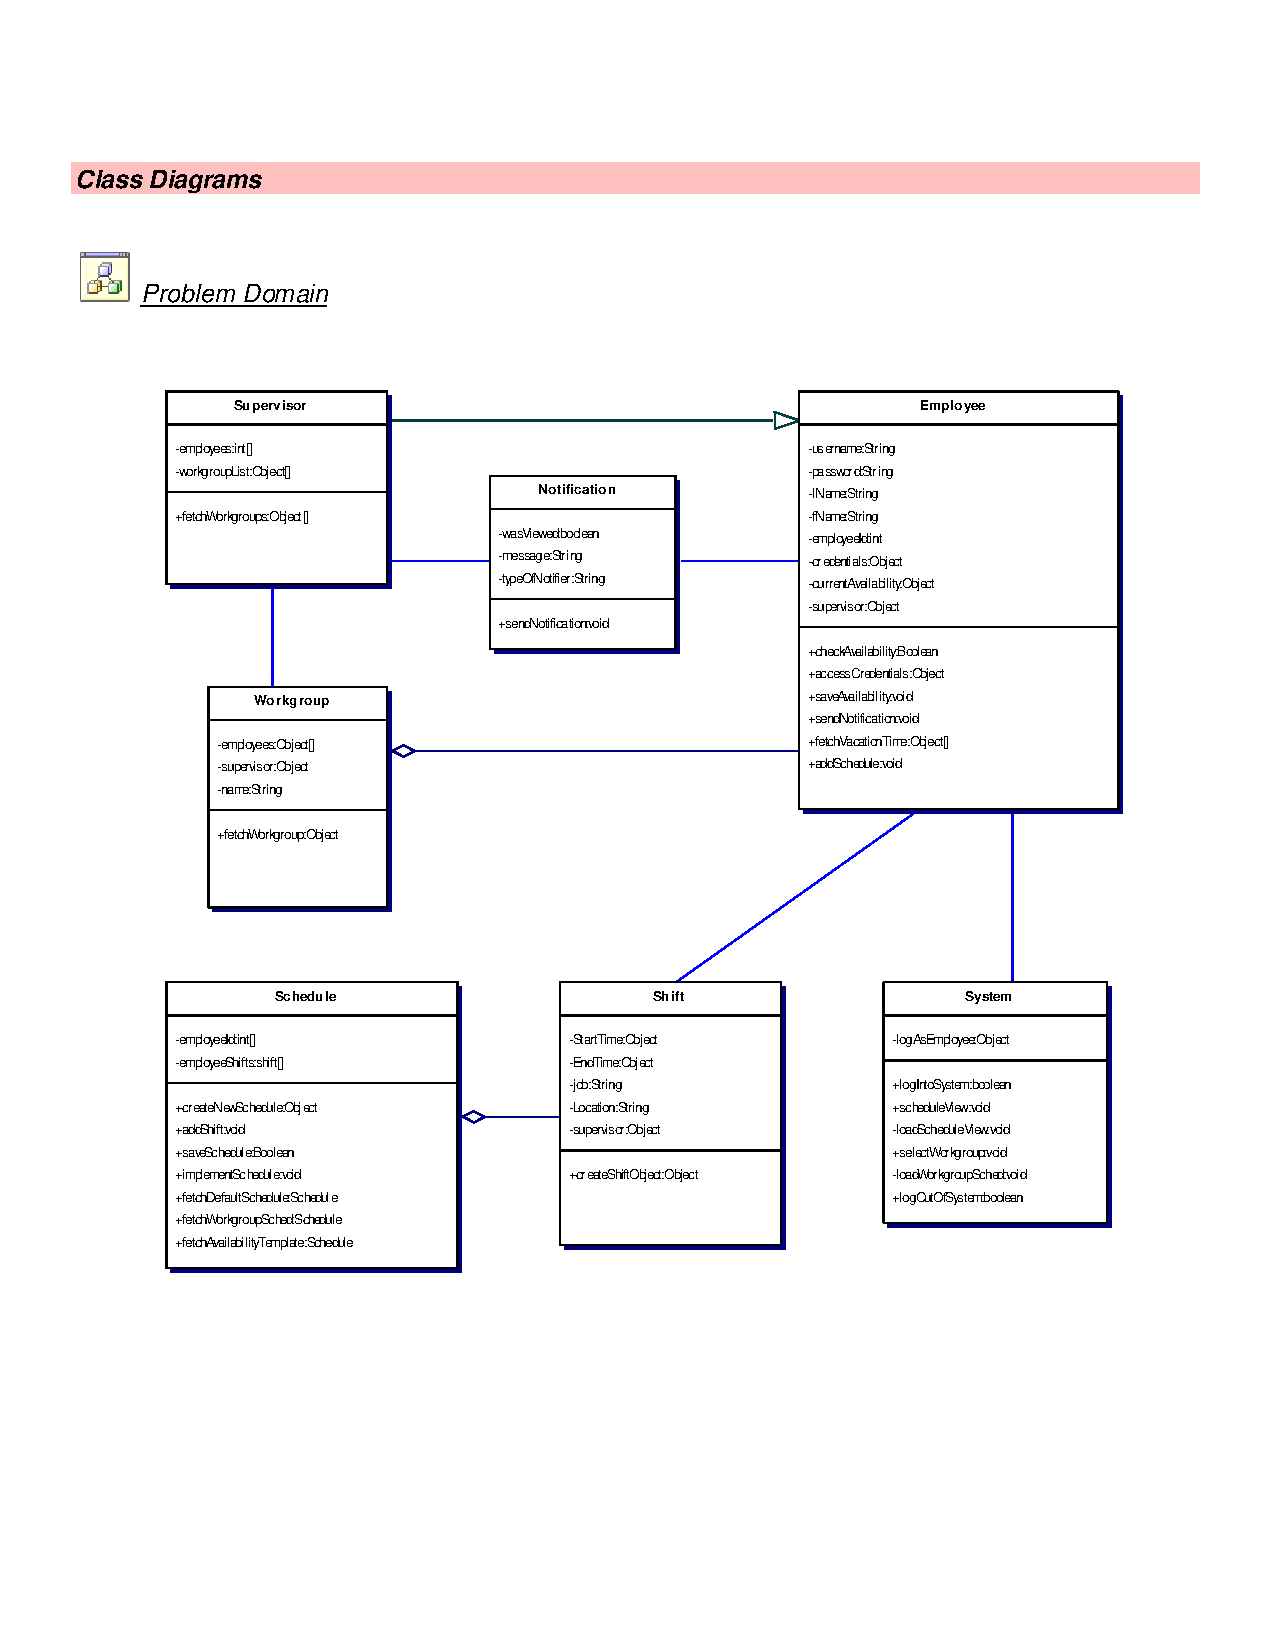
\includegraphics[scale=0.9,trim=10mm 60mm 25mm 20mm]{diagrams/cd_problem.pdf}
 \caption{\small
\textbf{Class Diagram} \space \newline The classes that are utilized by the system\index{system} with their respecive attributes}\label{fig:problemDomain}
\end{figure}
\newpage
\clearpage
\chapter{State Machine Diagrams}\index{State Machine Diagrams}
\section{State Machines}
\begin{figure}[htp]
 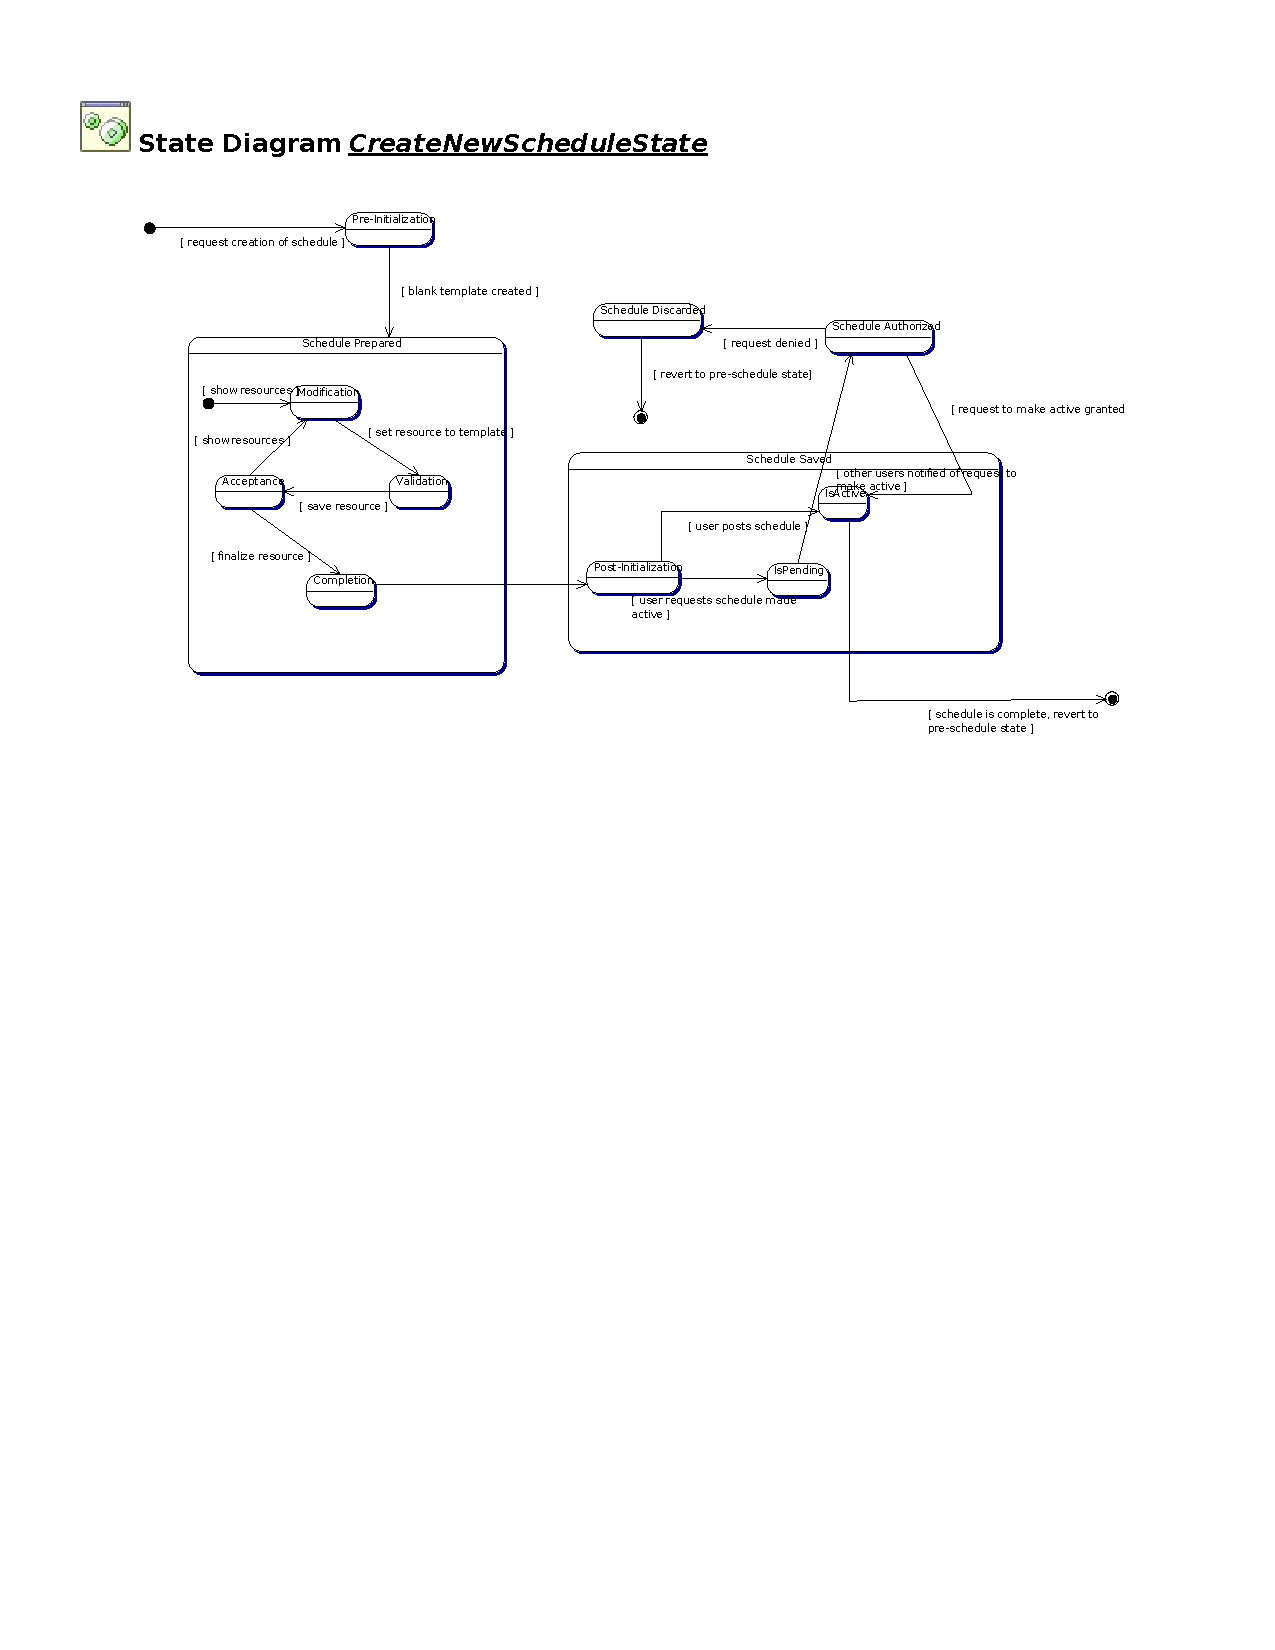
\includegraphics[trim=20mm 50mm 25mm 15mm]{externals/NewSchedState1.pdf}
 \caption{\small
\textbf{Create New \index{Schedule}Schedule State Diagram}\newline A representation of different states the system\index{system} goes through in creating a new  schedule}\label{fig:state1}
\end{figure}
\newpage
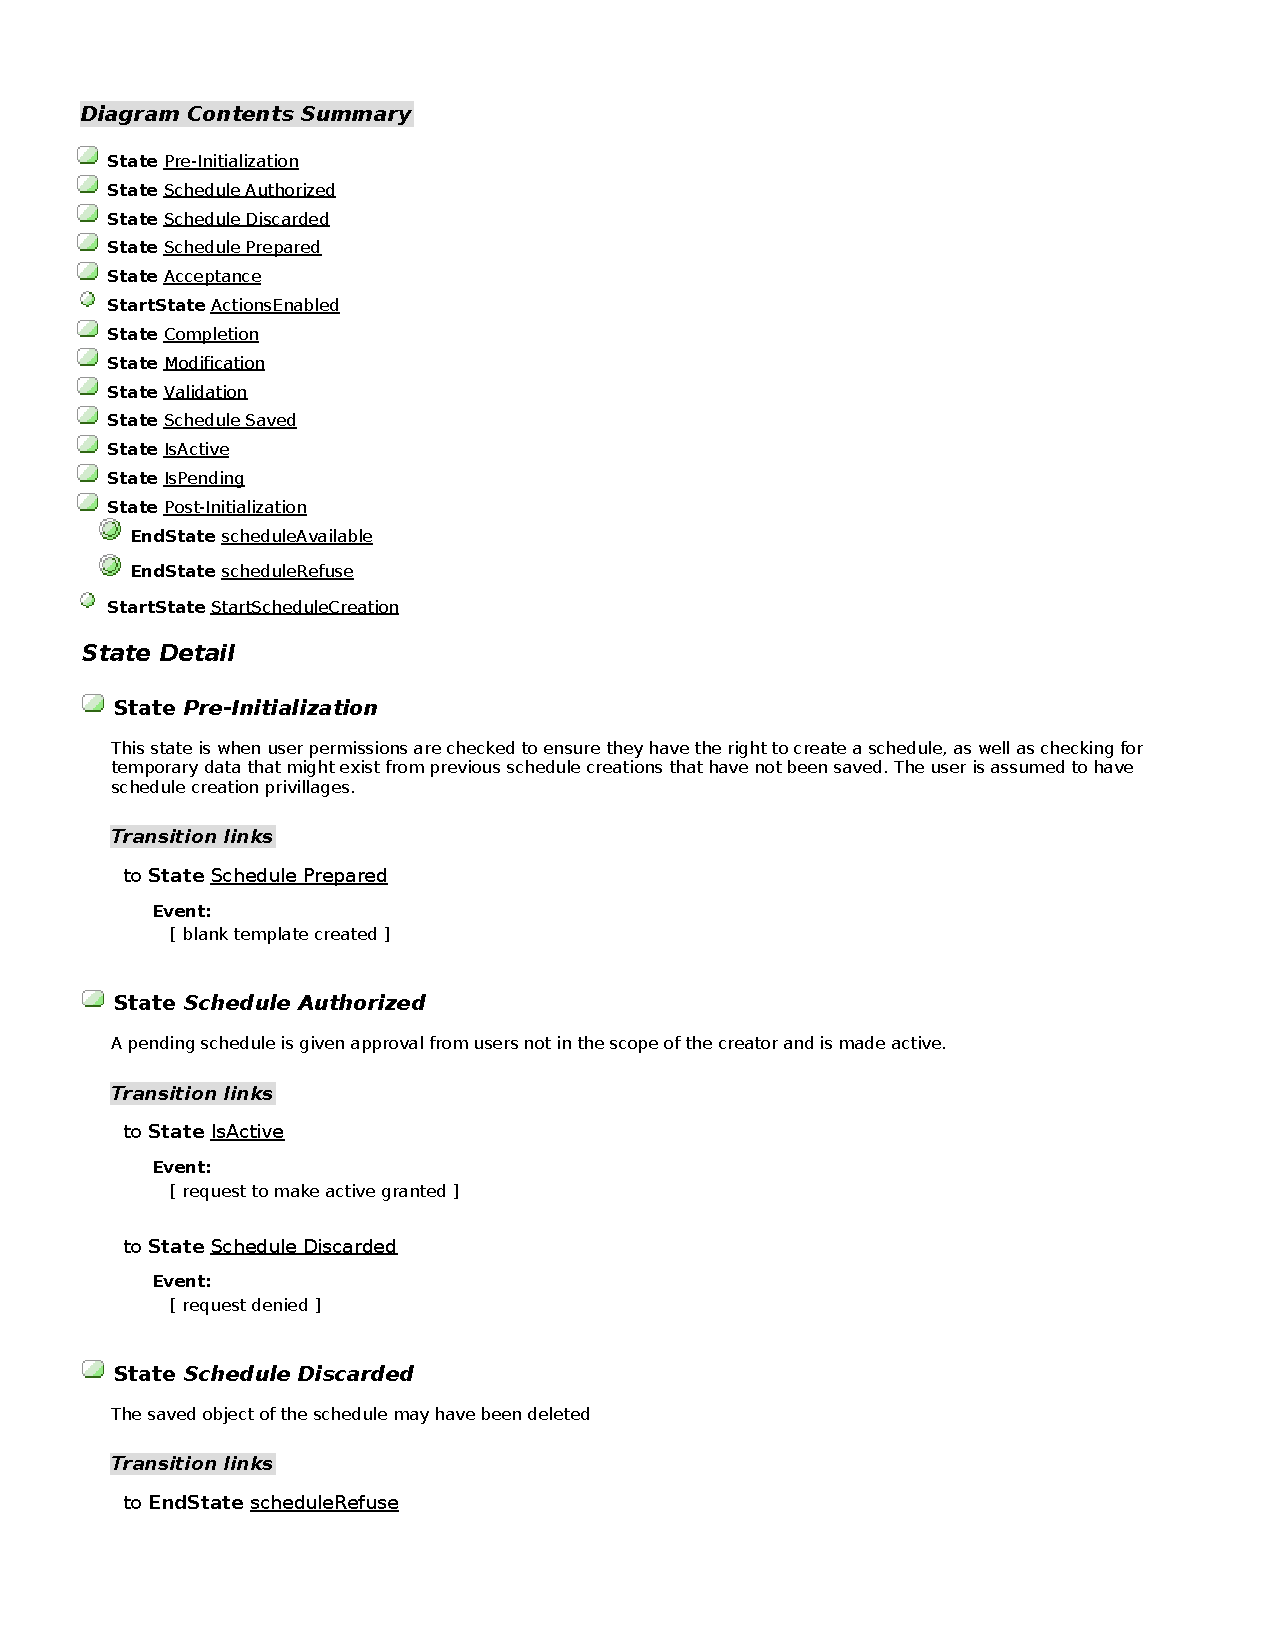
\includegraphics[scale=0.9,trim=20mm 30mm 25mm 20mm]{externals/NewSchedState2.pdf}
\newpage
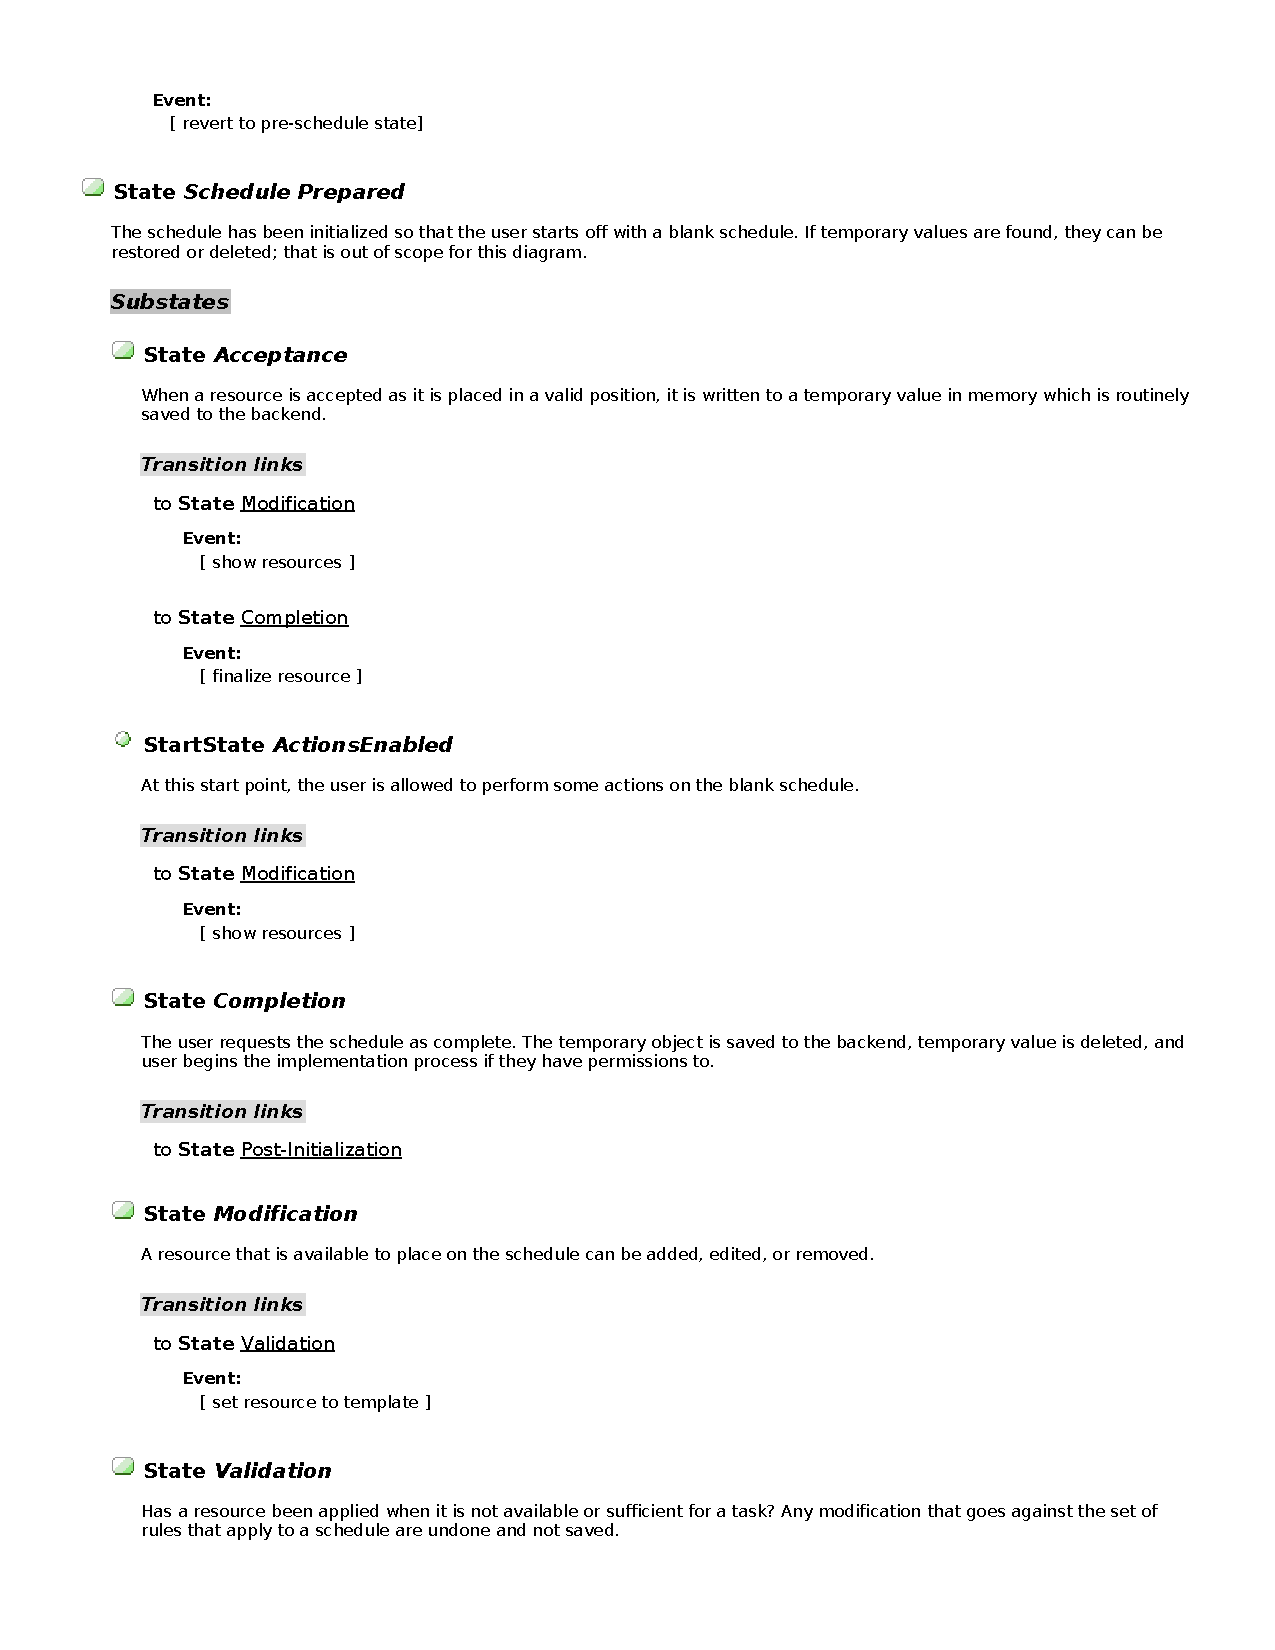
\includegraphics[scale=0.9,trim=20mm 30mm 25mm 20mm]{externals/NewSchedState3.pdf}
\newpage
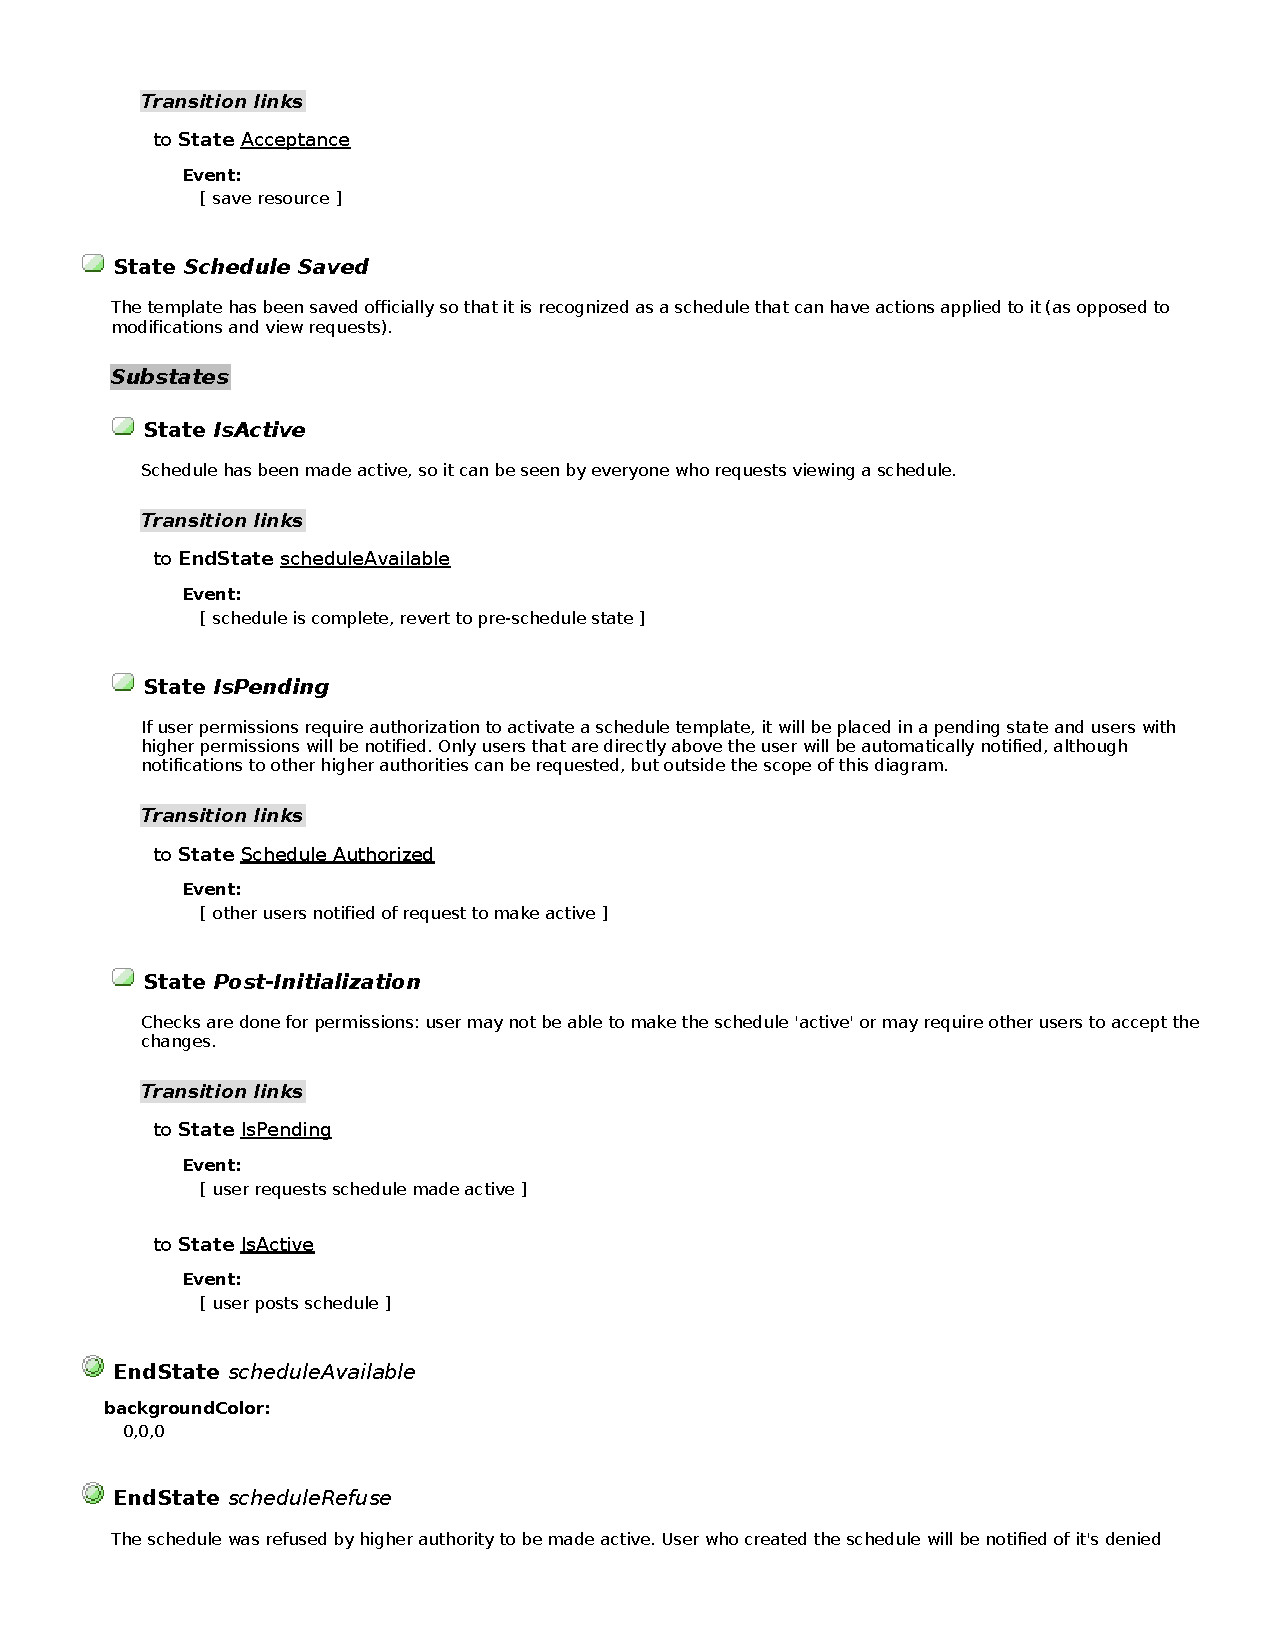
\includegraphics[scale=0.9, trim=20mm 30mm 25mm 20mm]{externals/NewSchedState4.pdf}
\newpage
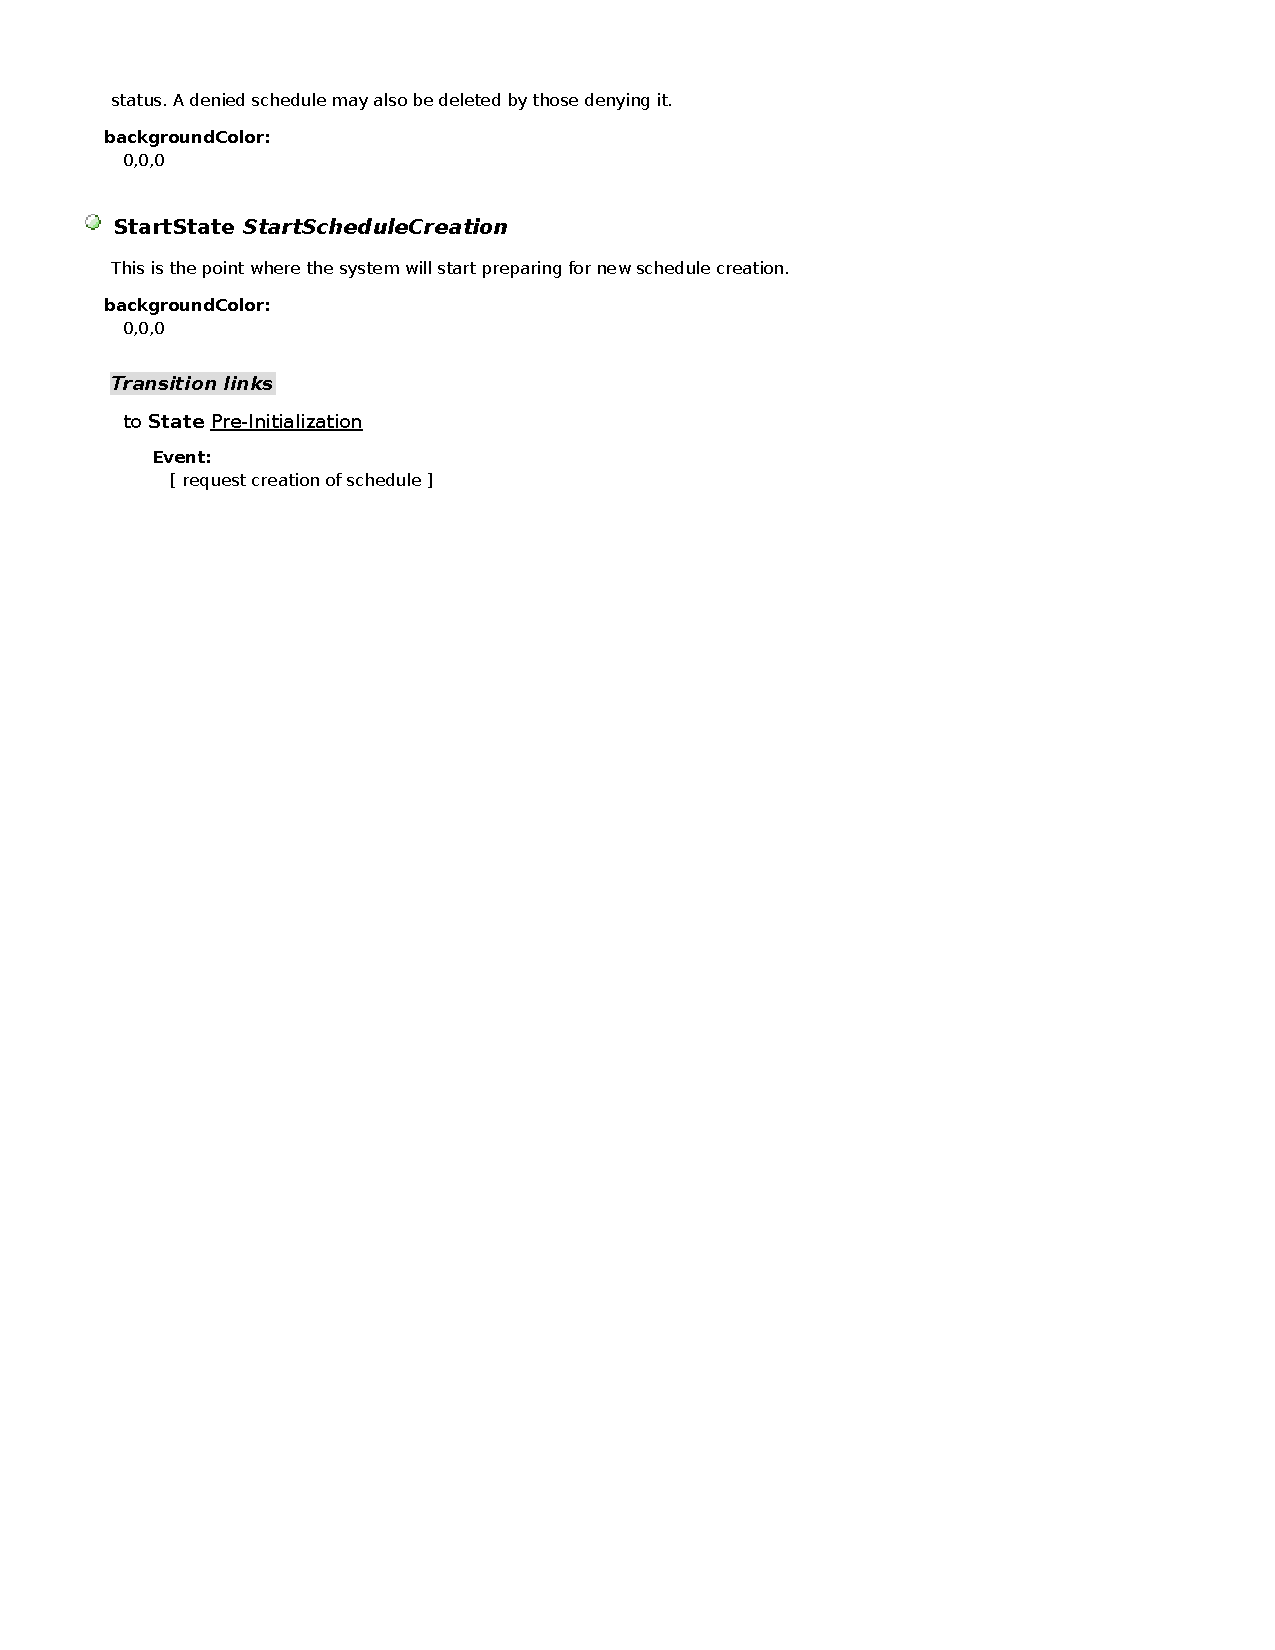
\includegraphics[scale=0.9,trim=20mm 30mm 25mm 20mm]{externals/NewSchedState5.pdf}
\newpage
\begin{figure}[htp]
 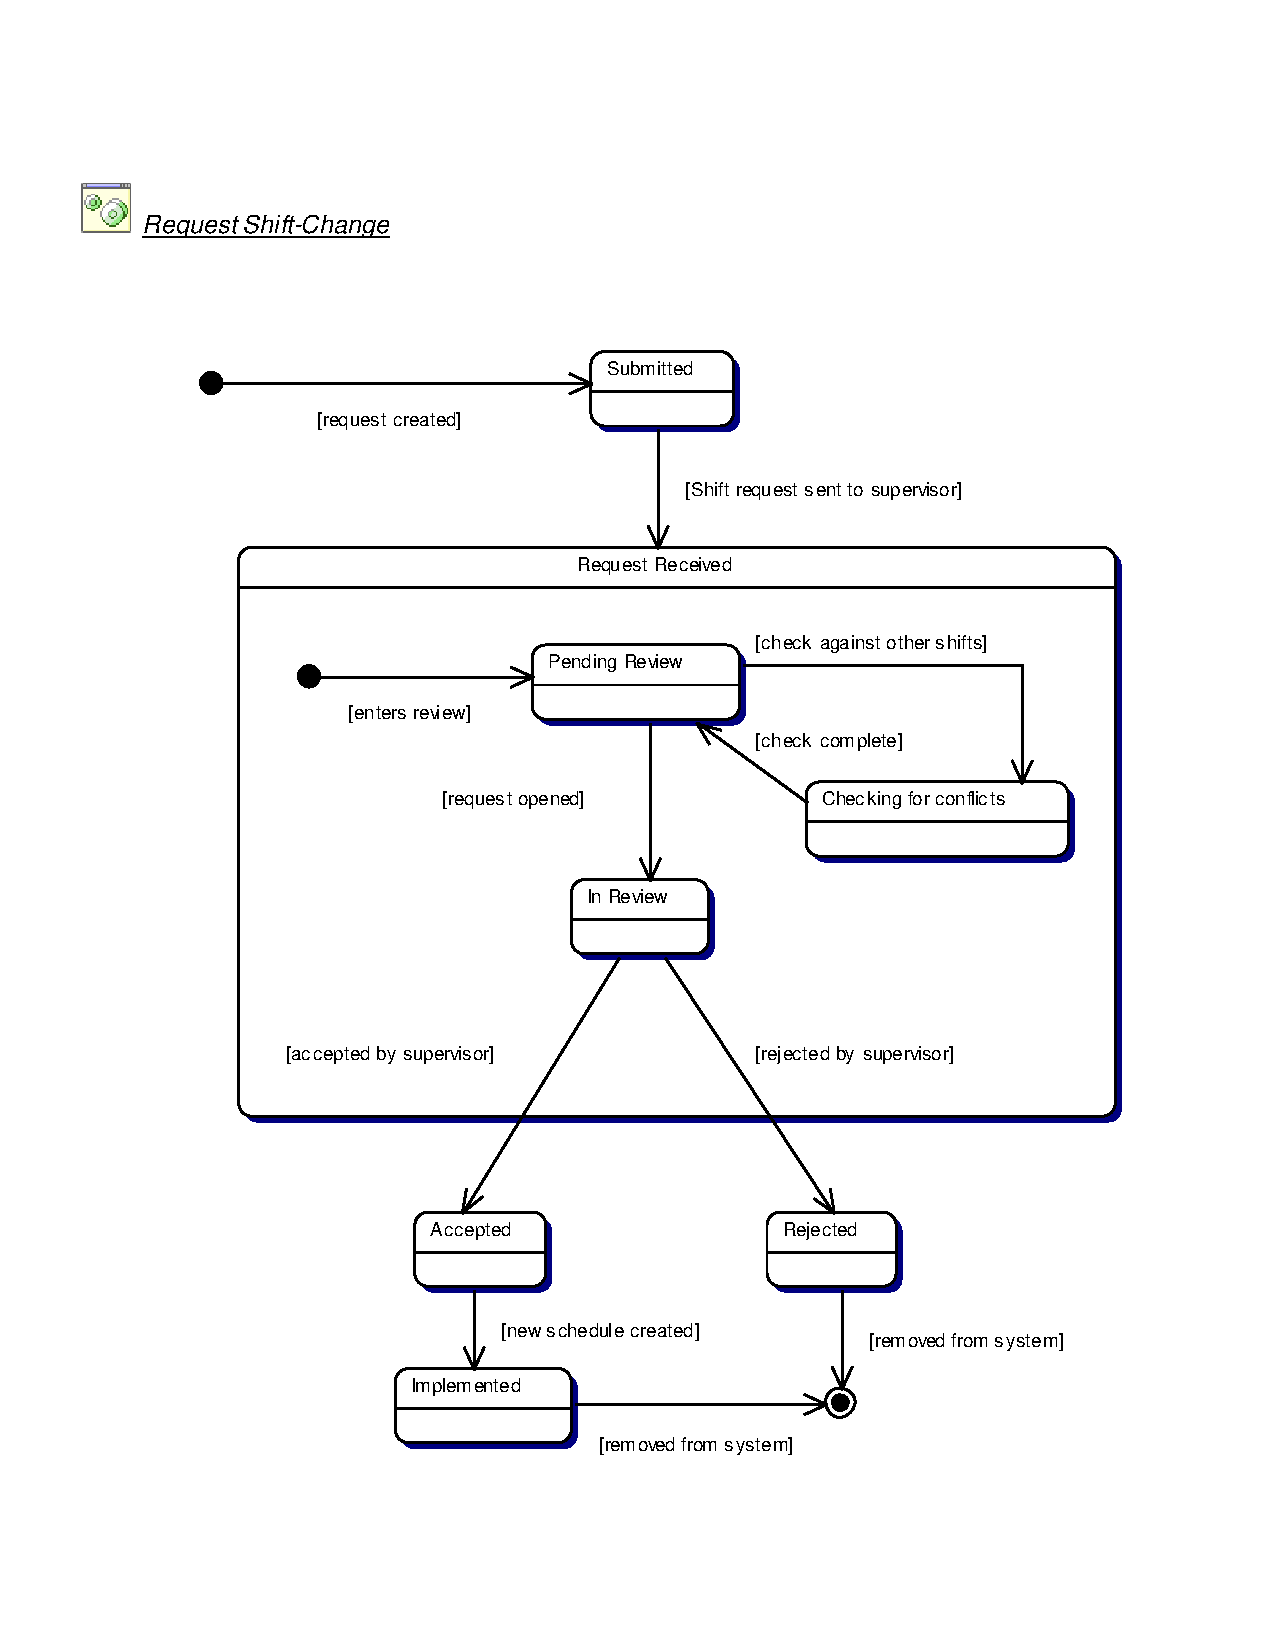
\includegraphics[scale=0.7,trim=20mm 20mm 25mm 30mm]{diagrams/ad_reqshift.pdf}
 \caption{\small
\textbf{Request \index{Shift Change}Shift Change State Diagram}\newline A representation of different states the system\index{system} goes through in allowing a user to request a shfit change}\label{fig:state2}
\end{figure}
\newpage
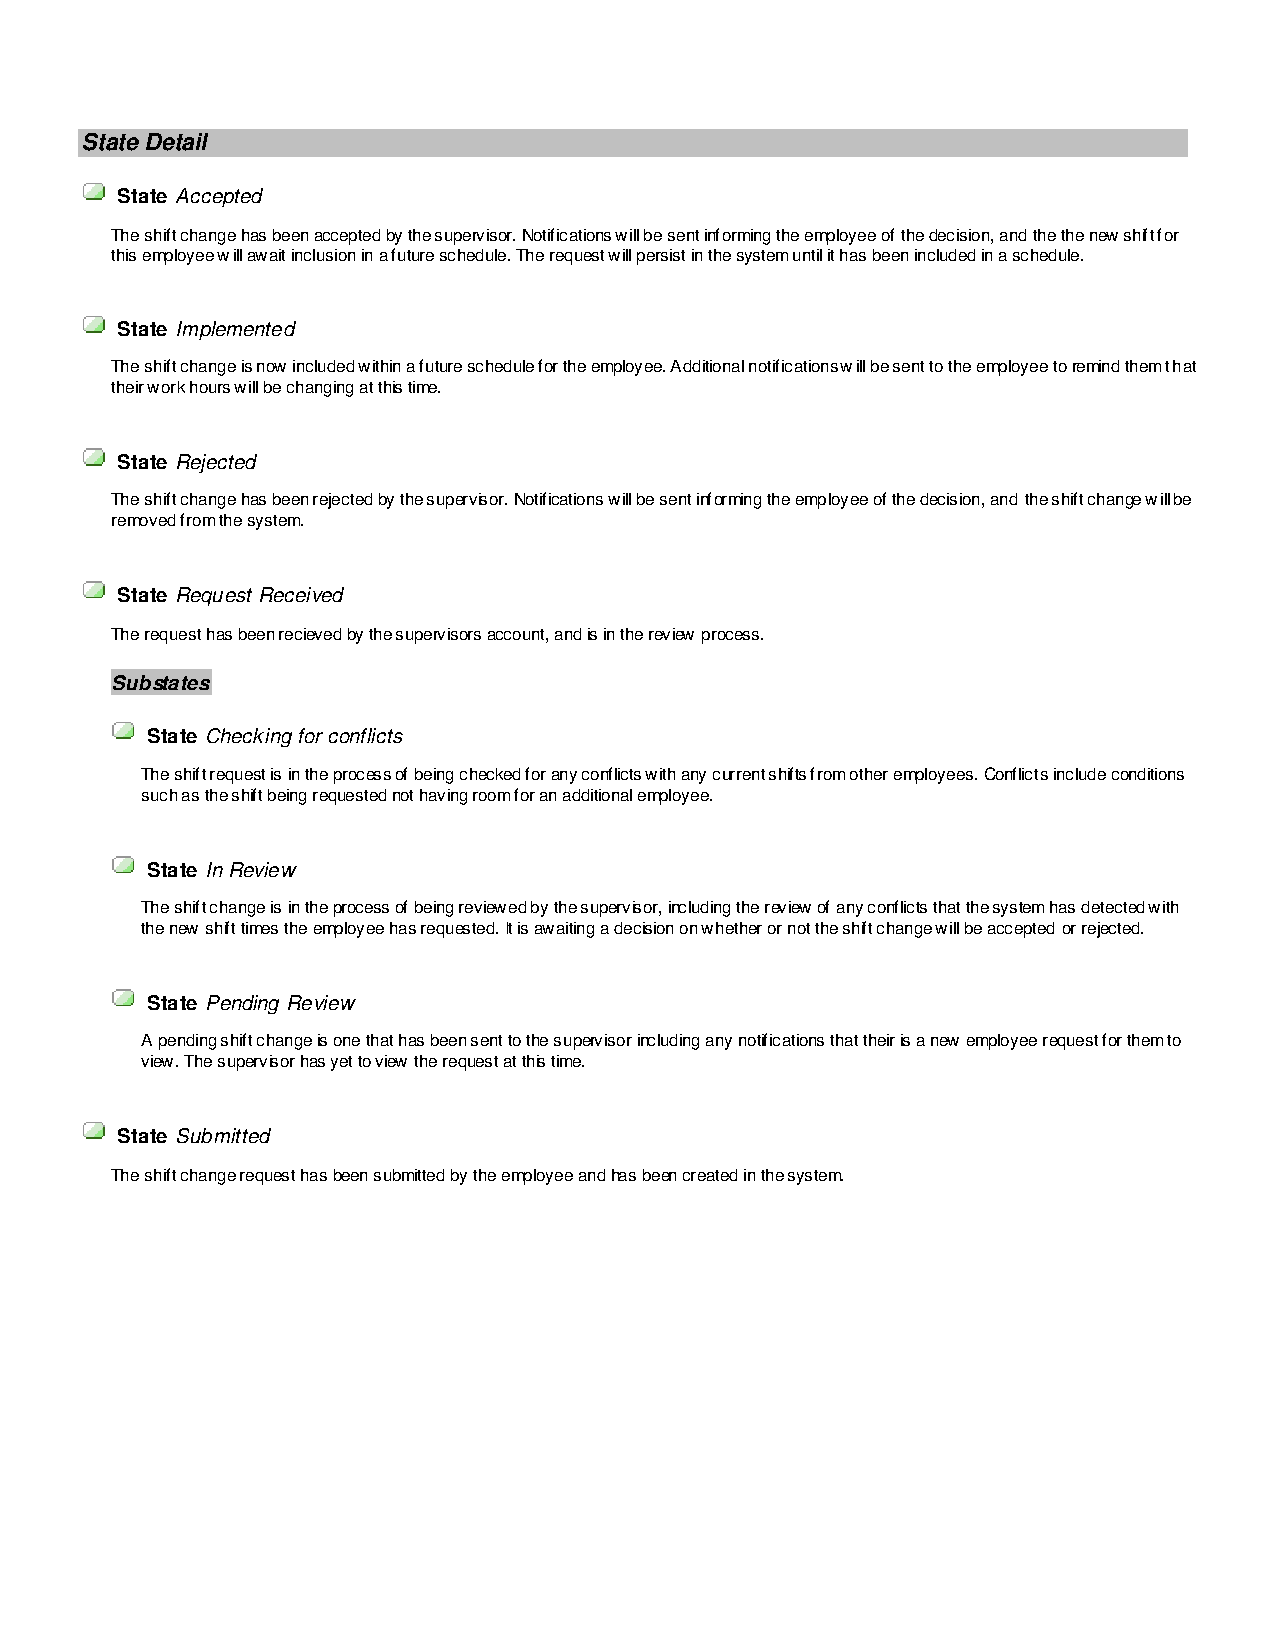
\includegraphics[scale=0.9,trim=15mm 20mm 25mm 20mm]{diagrams/ad_reqshift2.pdf}
\newpage
\begin{figure}[htp]
 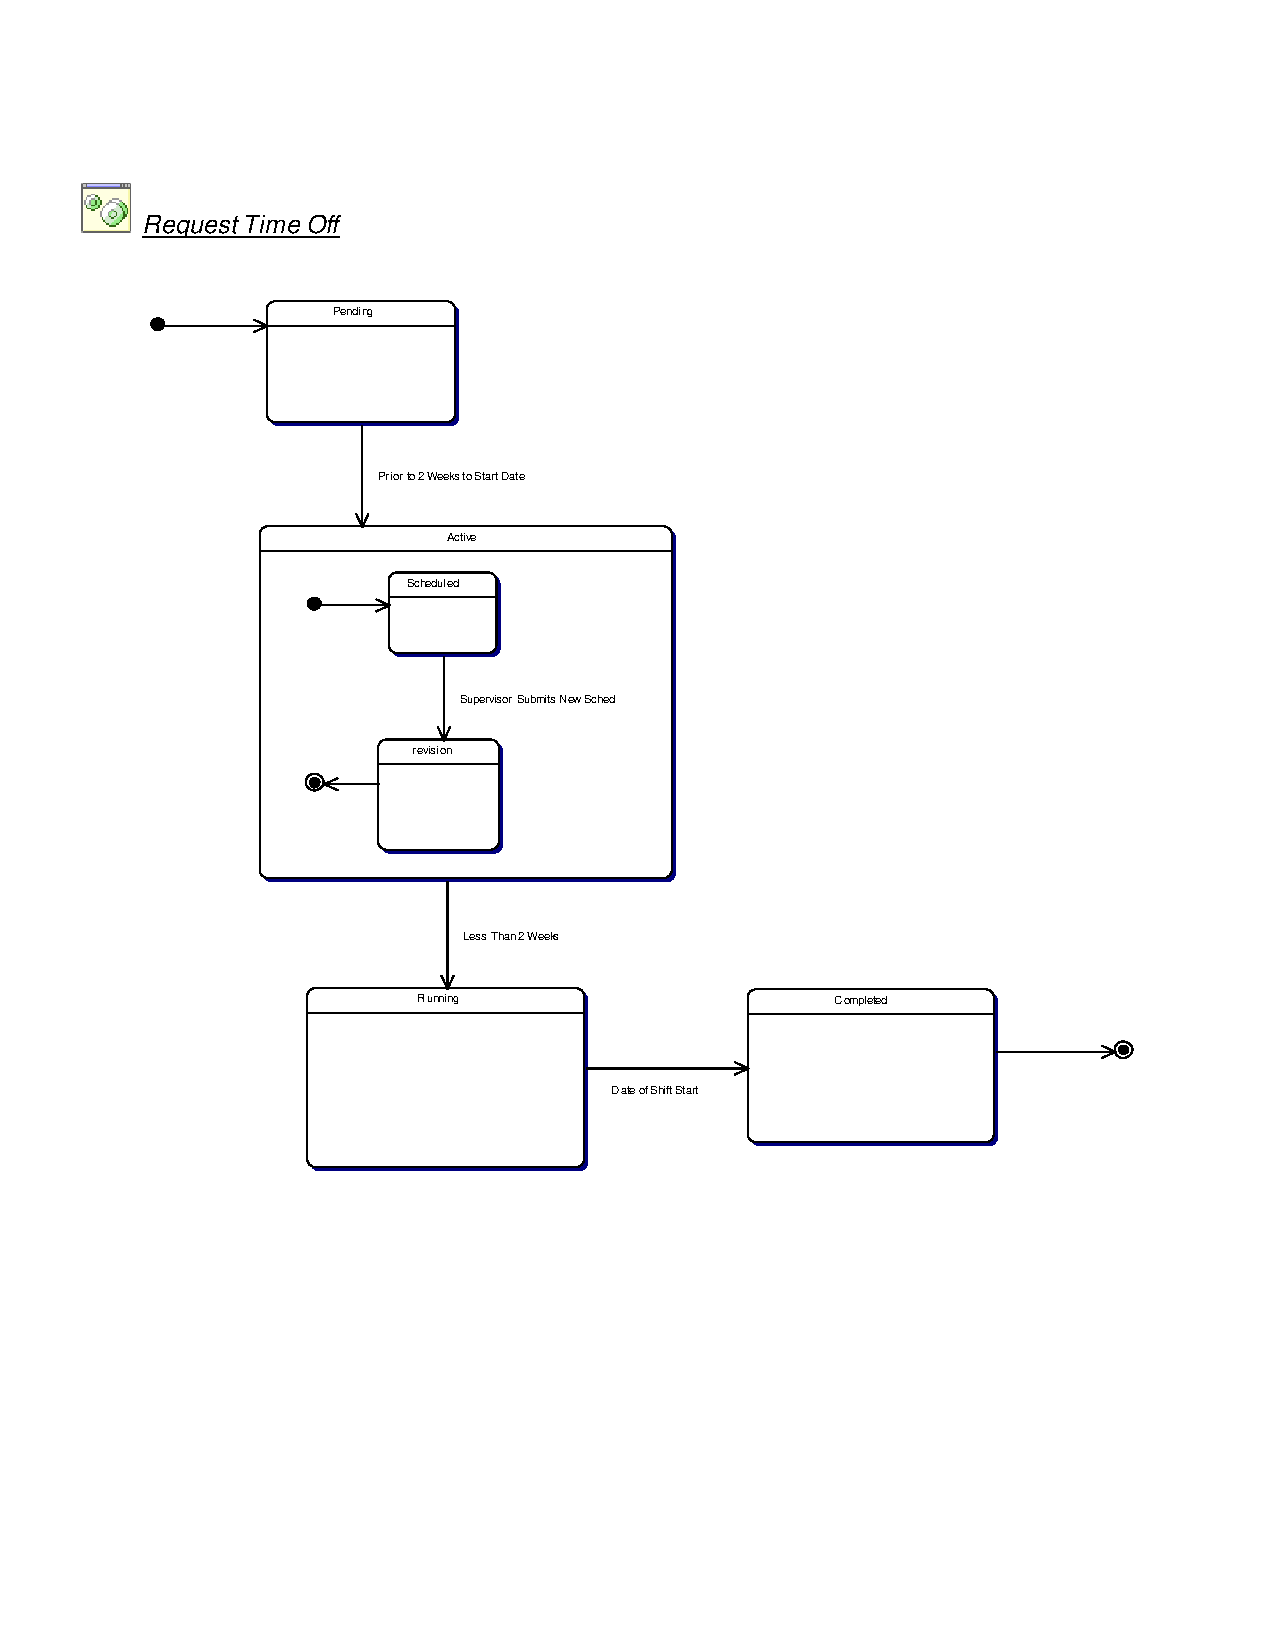
\includegraphics[scale=0.8,trim=15mm 70mm 25mm 20mm]{diagrams/reqtimeoff.pdf}
 \caption{\small
\textbf{Request Time Off State Diagram}\newline A representation of different states the system\index{system} goes through when an employee requests time off}\label{fig:state3}
\end{figure}
\pagebreak
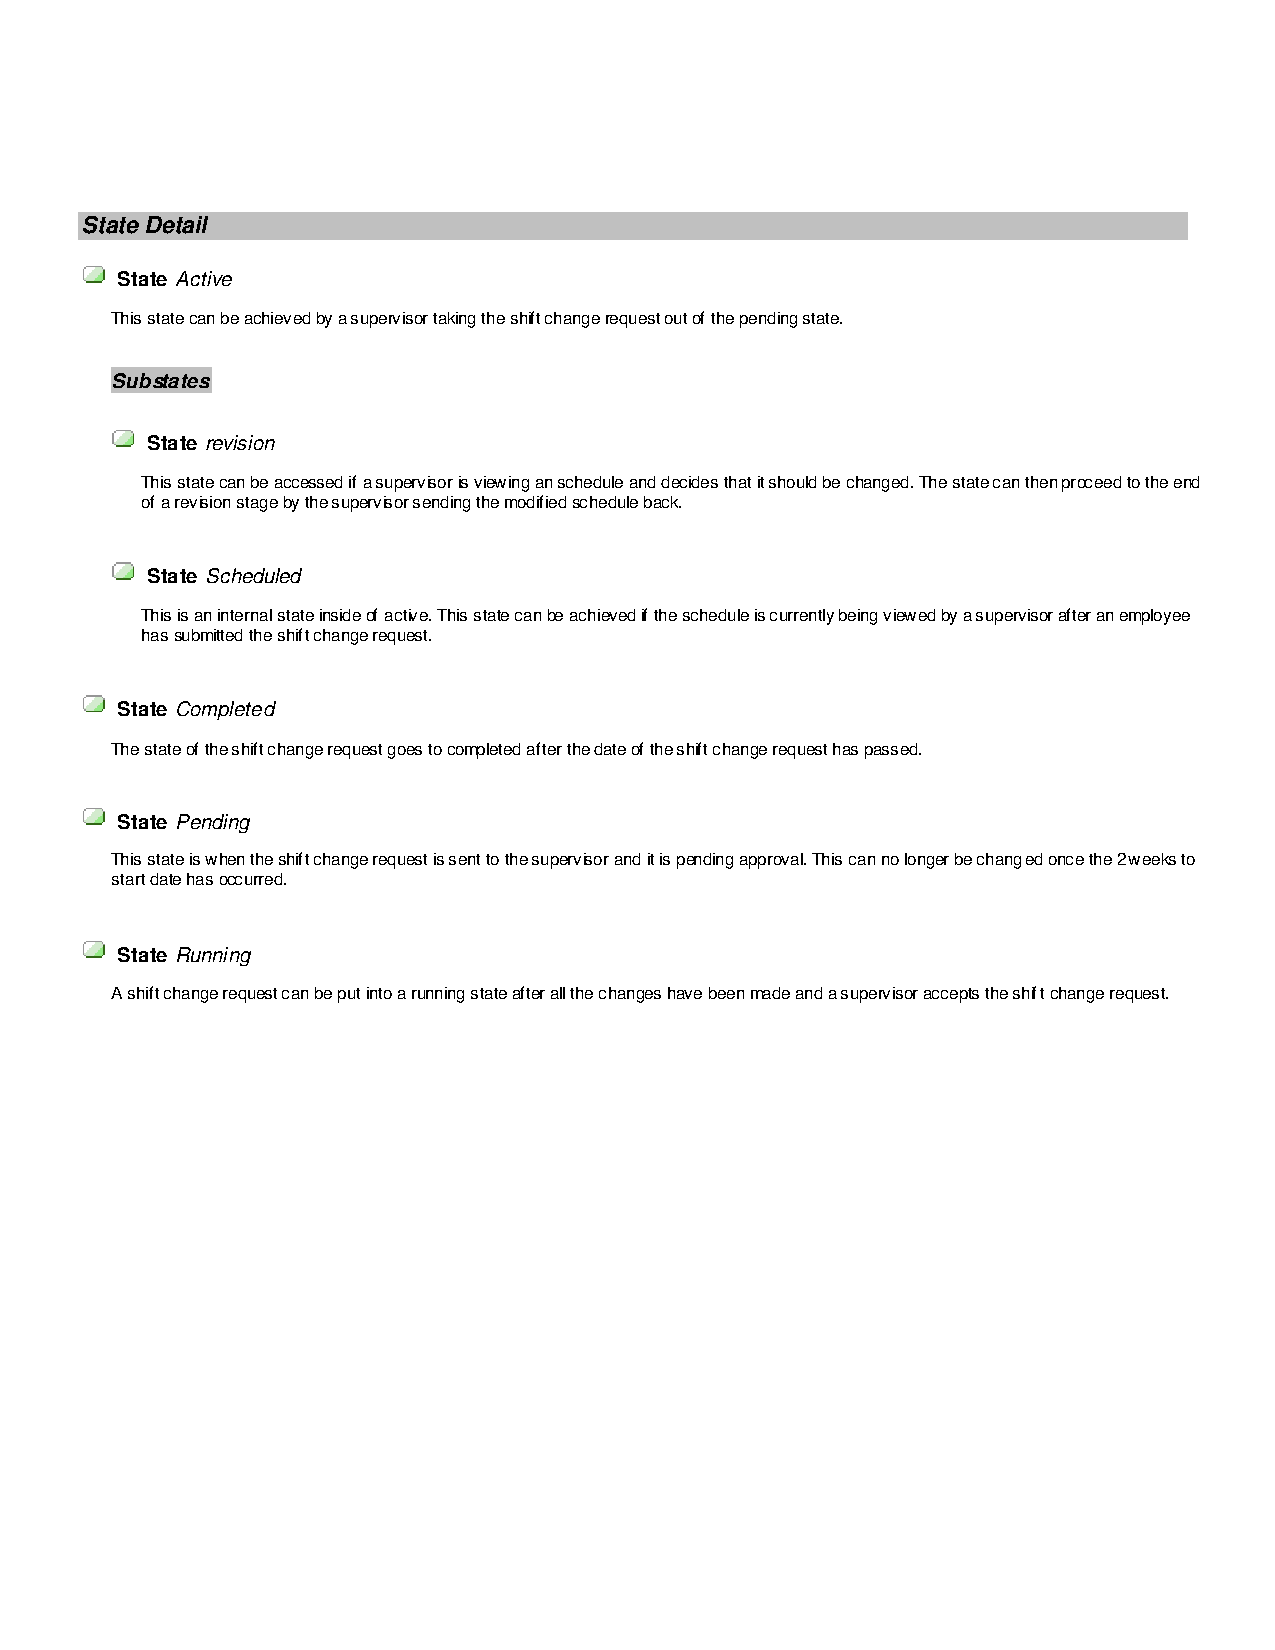
\includegraphics[scale=0.9,trim=15mm 30mm 25mm 20mm]{diagrams/reqtimeoff2.pdf}
\newpage
\clearpage
\chapter{Activity Diagrams}\index{Activity Diagrams}
\newpage
\section{Activity Diagrams}
\begin{figure}[hbp]
 \centering
 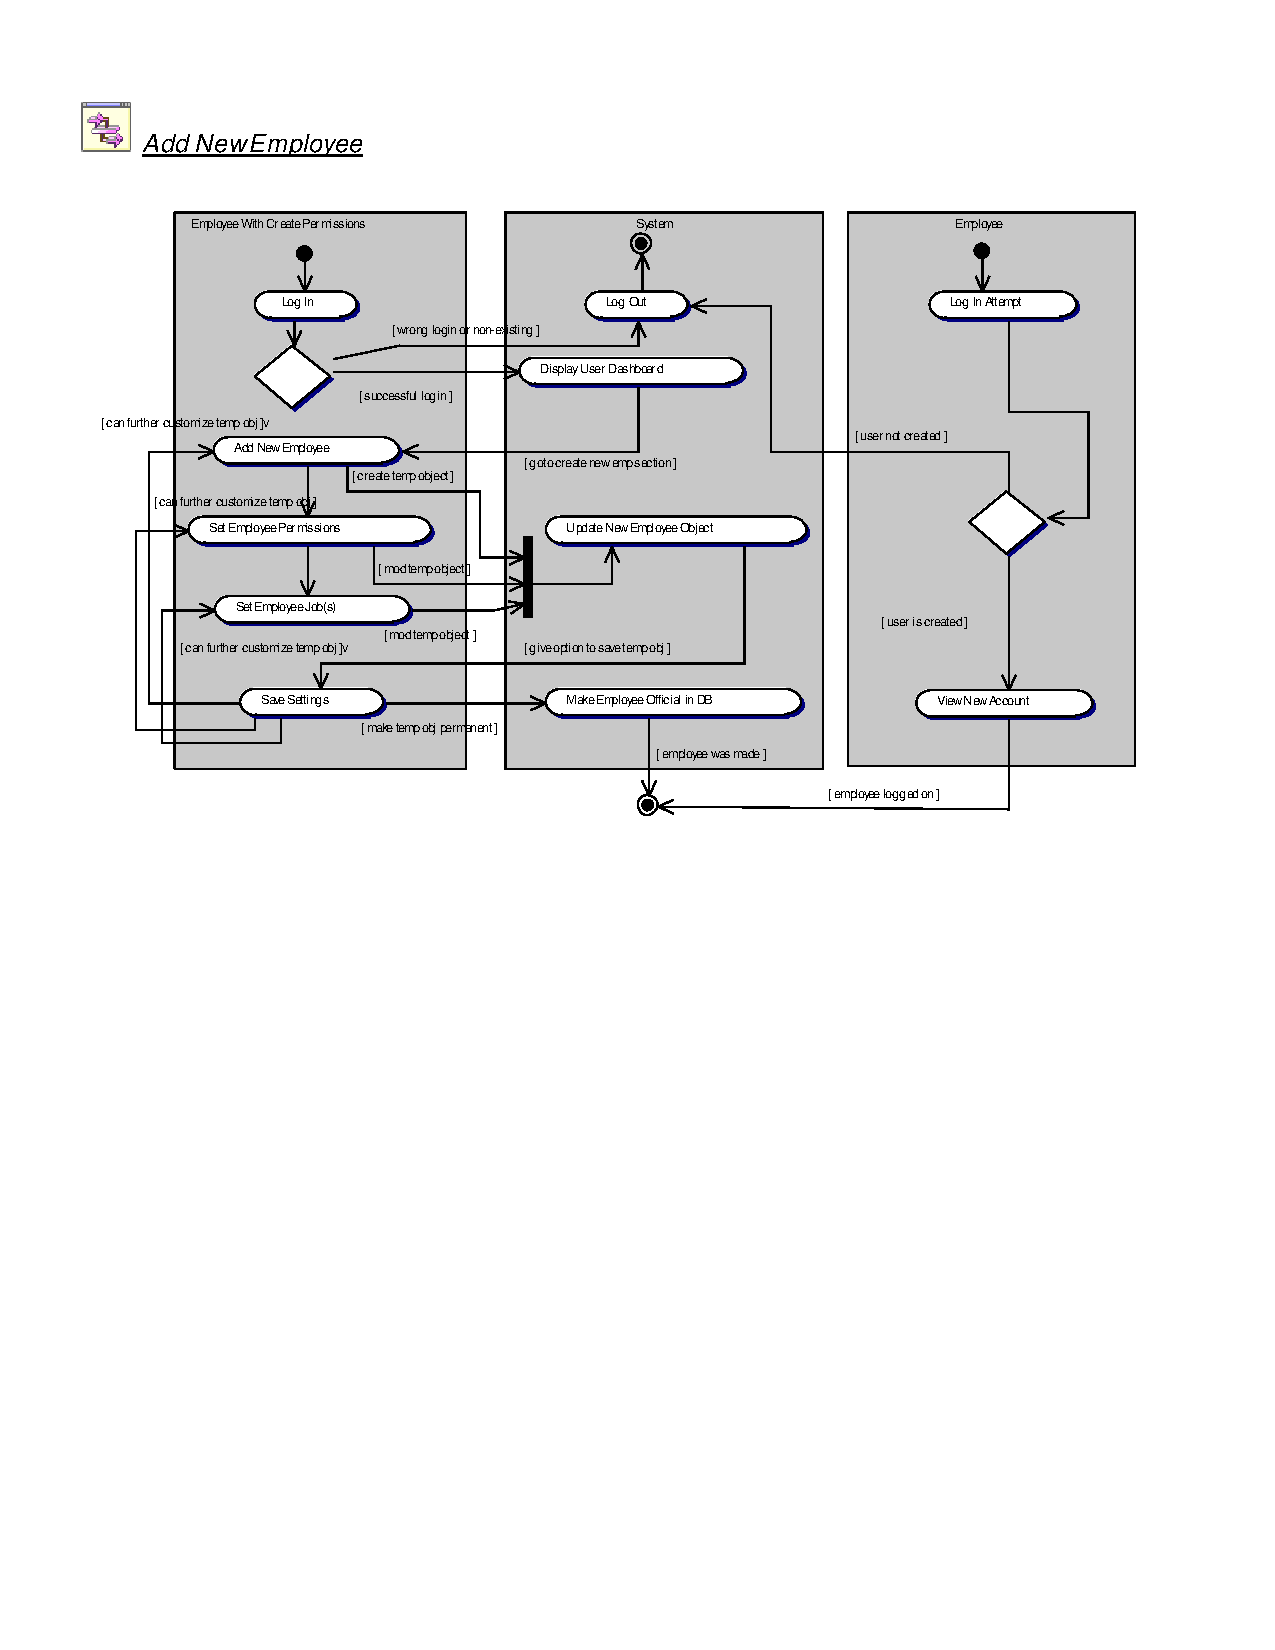
\includegraphics[scale=0.9,trim=20mm 100mm 25mm 10mm]{diagrams/ad_add1.pdf}
 \caption{\small
\textbf{Add New Employee Activity Diagram}\newline The actions required in order to add a new employee to the \index{WebAgenda} system\index{system}}\label{fig:act1}
\end{figure}
\newpage
\begin{figure}[activity_genrep]
 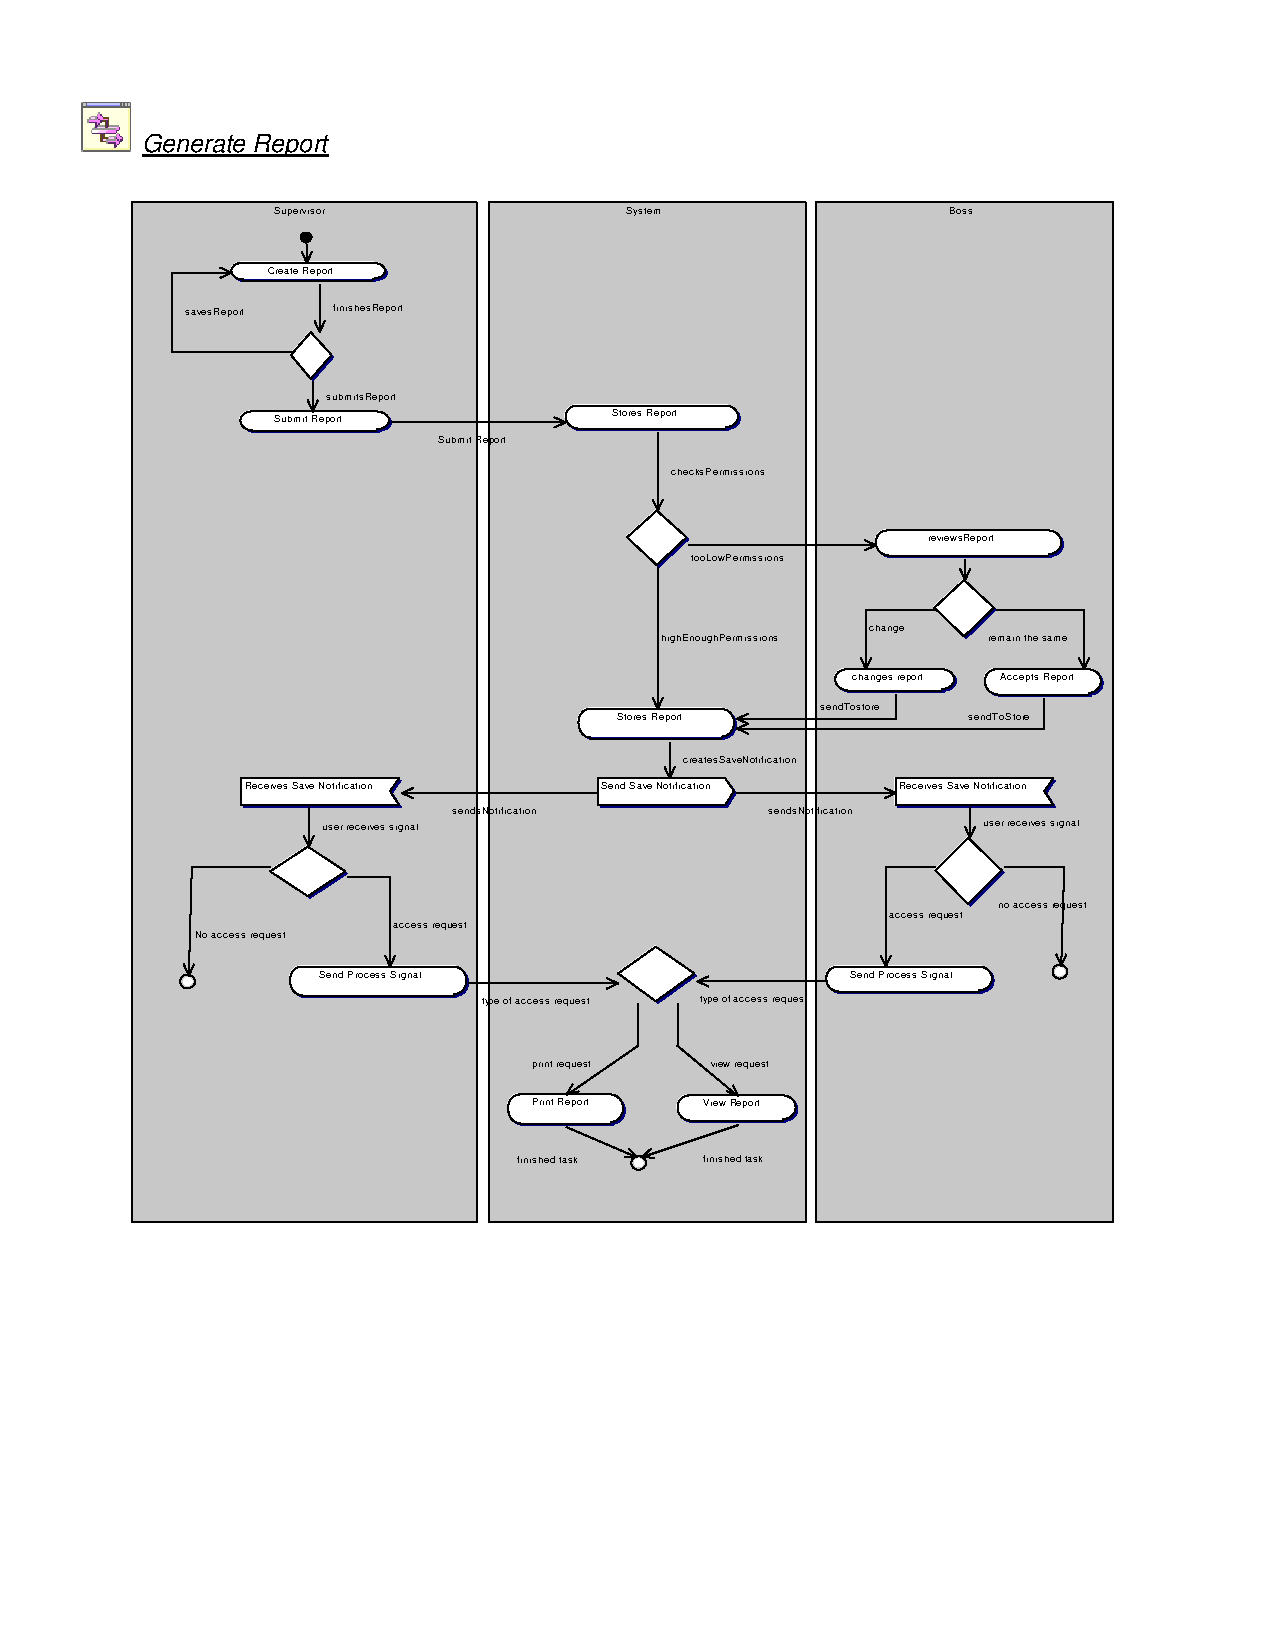
\includegraphics[trim=20mm 70mm 25mm 15mm]{diagrams/ad_gen1.pdf}
 \caption{\small
\textbf{Generate Report Activity Diagram}\newline The actions required to generate detailed and relevant reports}\label{fig:act2}
\end{figure}
\newpage
\begin{figure}[activity_reqshiftchng]
 \centering
 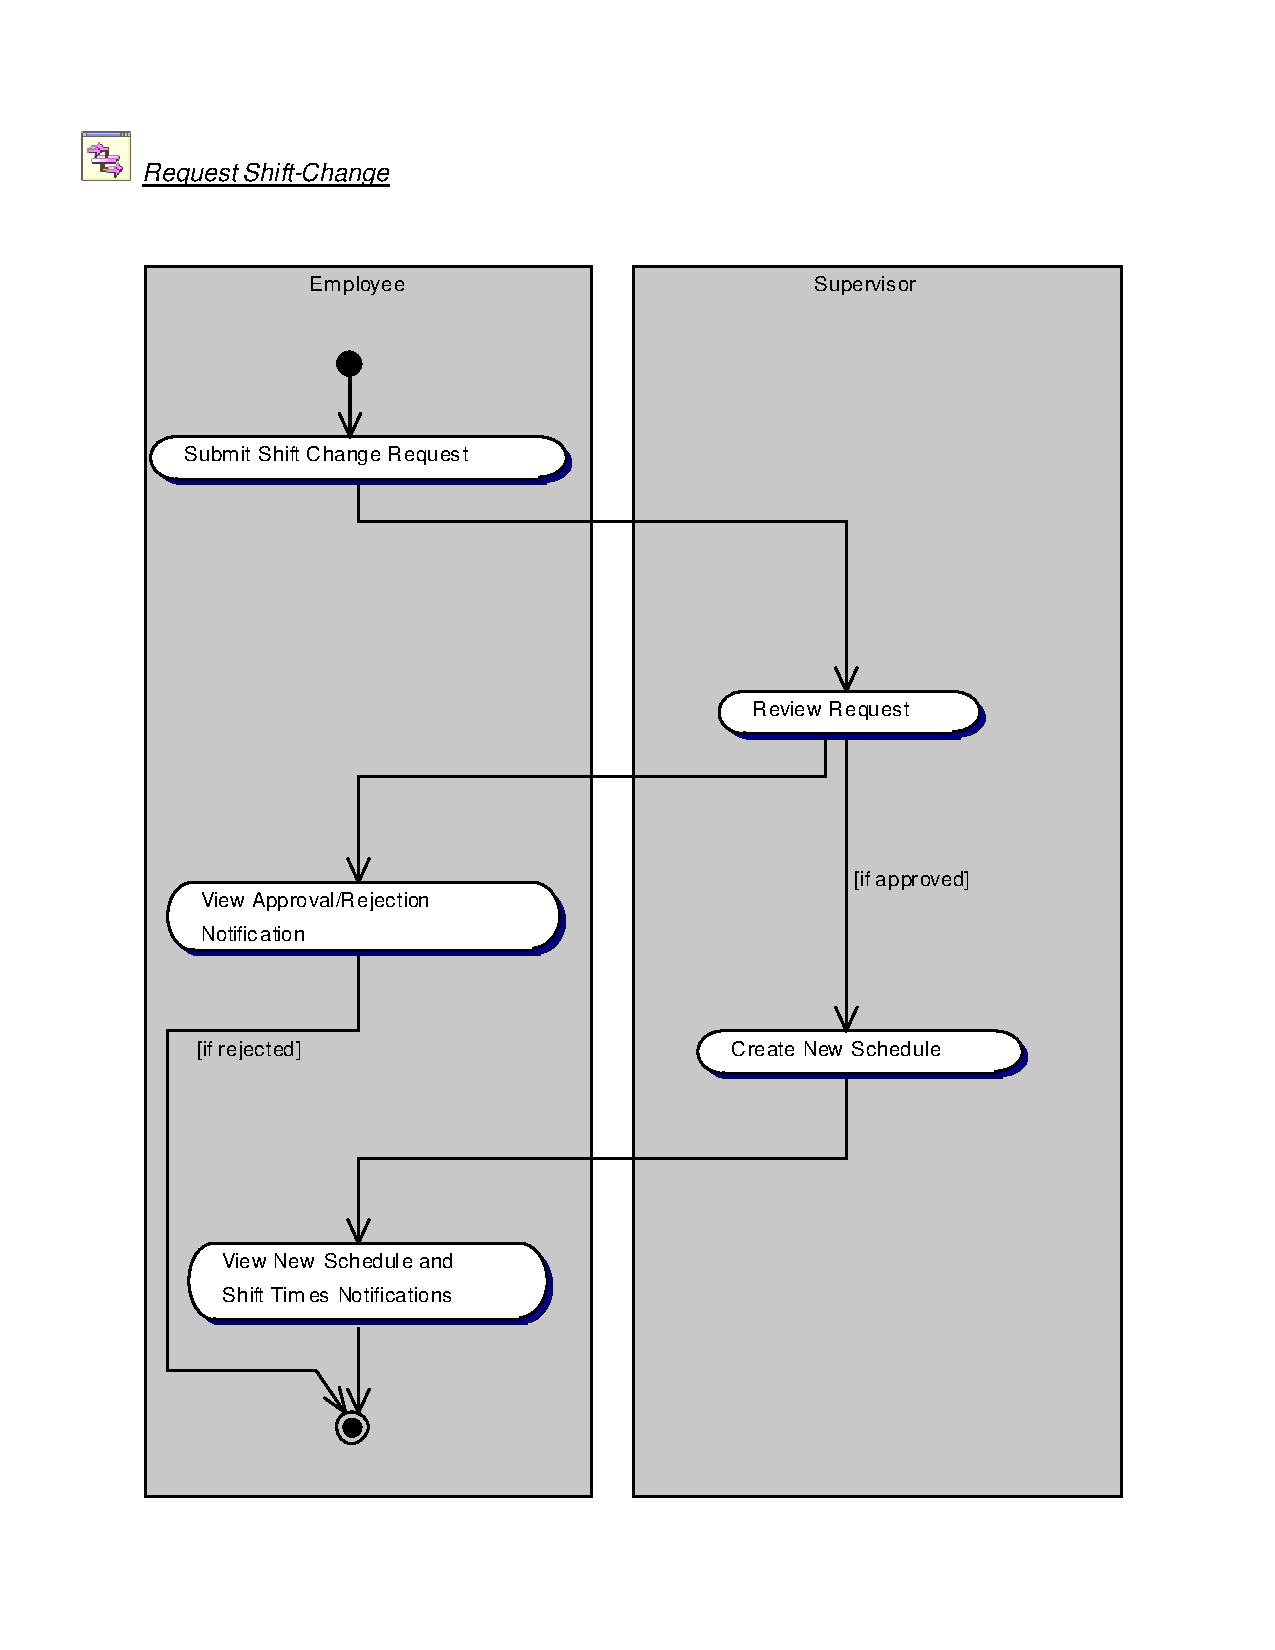
\includegraphics[scale=0.8,trim=20mm 20mm 25mm 0mm]{diagrams/swimreq.pdf}
 \caption{\small
\textbf{Request Shift Change Activity Diagram}\newline This diagram shows the status of a shift change request, from being created by an employee, reviewed by a supervisor, and being implemented in future schedules or removed from the system\index{system}. }\label{fig:act3}
\end{figure}
\newpage
\begin{figure}[activity_exchangeshifts]
 \centering
 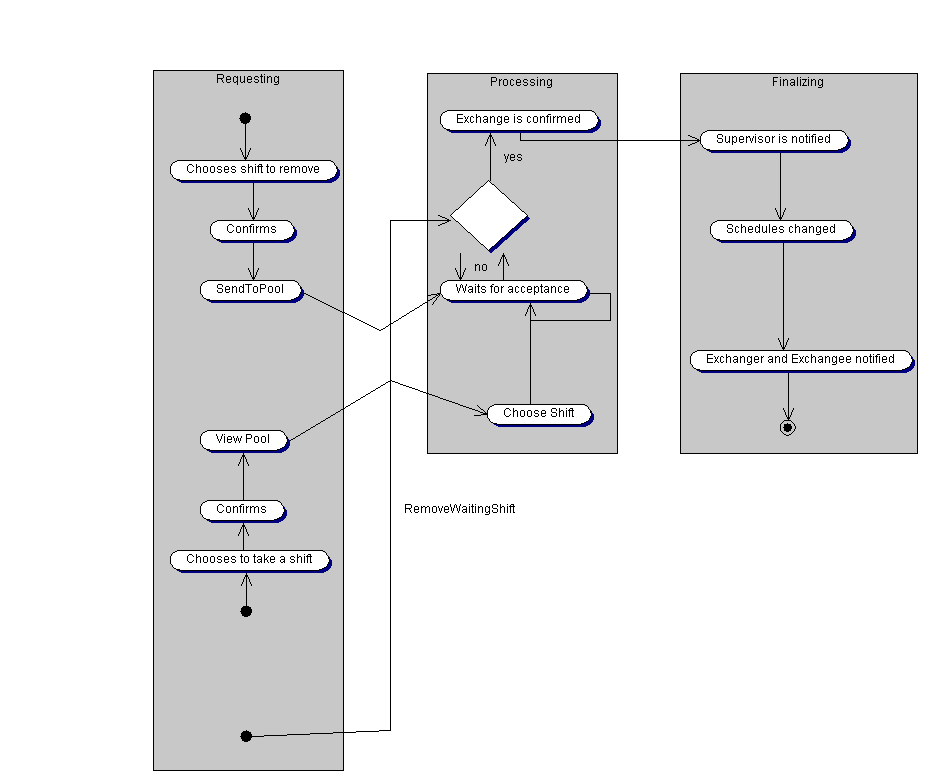
\includegraphics[scale=0.79,trim=40mm 0mm 0mm 0mm]{diagrams/actRequestShiftChange.png}
 \caption{\small
\textbf{Shift Exchange Activity Diagram}\newline This diagram shows the status of a shift being exchanged or given to another employee. }\label{fig:actRequestShiftChange}
\end{figure}
\newpage

\part{System Design}
\chapter{Layered Architecture}
\section{Package Diagram}
\pagebreak
\begin{figure}[packageDiagram]
 \centering
 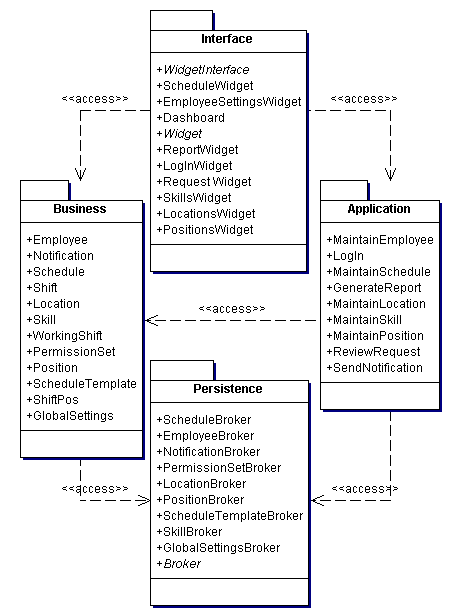
\includegraphics[scale=0.8]{externals/PackageDiagram.png}
 \caption{\small
\textbf{Package Diagram}\newline This diagram shows all the packages and objects included in the system }\label{fig:packageDiagram}
\end{figure}

\chapter{Persistence Model}
\section{Textual Description Document}
\subsection*{Control Classes}
\paragraph*{}\hspace{0.6cm}Our system\index{system} will have control classes and brokers that will be in charge of directly interacting with the database\index{Database}. The control pattern will implement the application logic layer of our system. Any insertion, deletion or updating of data occurs with the assistance of these classes. The control classes are also used to perform any interaction with the interface\index{interface} and problem domain layers. Basically they are the link between the physical data in the database and what the user sees in the end. The broker classes are in place to put forth an application programming interface to allow developers to get data from the database without directly interacting with the data. This is in place to ensure that the data integrity of the database stays consistent throughout system\index{system} use. Ensuring data integrity is a key aspect of a system\index{system} with a four-tier architecture. Allowing the developers to access direct data and information from the database without physically letting them grab the data is the key point of having the control classes.\newline
\paragraph*{}\hspace{0.6cm}The interface layer is implemented in the interface\index{interface} classes which will be used to communicate with the users in an easy to use fashion. The interface classes will then interpret the user interaction and send that parsed information to the broker classes to get the information that the user requested. From there the interface class will parse the information received from the broker classes back into a format that the user can understand and interact with.\newline
\paragraph*{}\hspace{0.6cm}The business layer consists of data that represents real life objects that interact with each other and peristance layer classes.
\paragraph*{}\hspace{0.6cm}The persistence classes will be used as direct data from the database\index{Database}. Mostly consists of objects that are persisted into the database as actual data. The persistence classes will be hidden from the developers due to the broker classes. So in fact, the developers will not be able to directly interact with these classes without first going through the broker classes. This again, is to ensure data integrity in the persistence layer and at the physical data layer.
\paragraph*{}\hspace{0.6cm}The application layer contains classes that control the flow of how the interface and business objects interact. While the Broker manages back-end processes, application manages front-end proceses including validation.
\pagebreak
\section{Entity Relationship Diagrams}
\pagebreak
{
\begin{figure}[ConceptualERD]
 \centering
 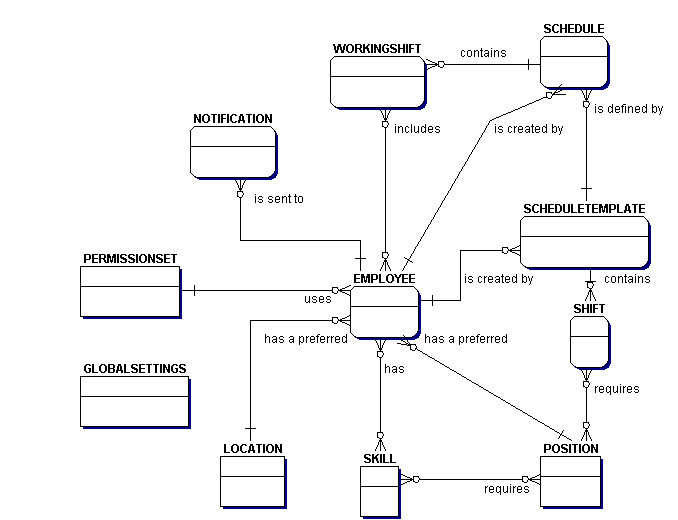
\includegraphics[scale=0.8,trim=30mm 00mm 20mm 10mm]{externals/ConceptualERD.png}
 \caption{\small
\textbf{Conceptual ERD Diagram}}\label{fig:conceptERD}
\end{figure}
\pagebreak
\newpage
\begin{figure}[ImplementationERD]
 \centering
 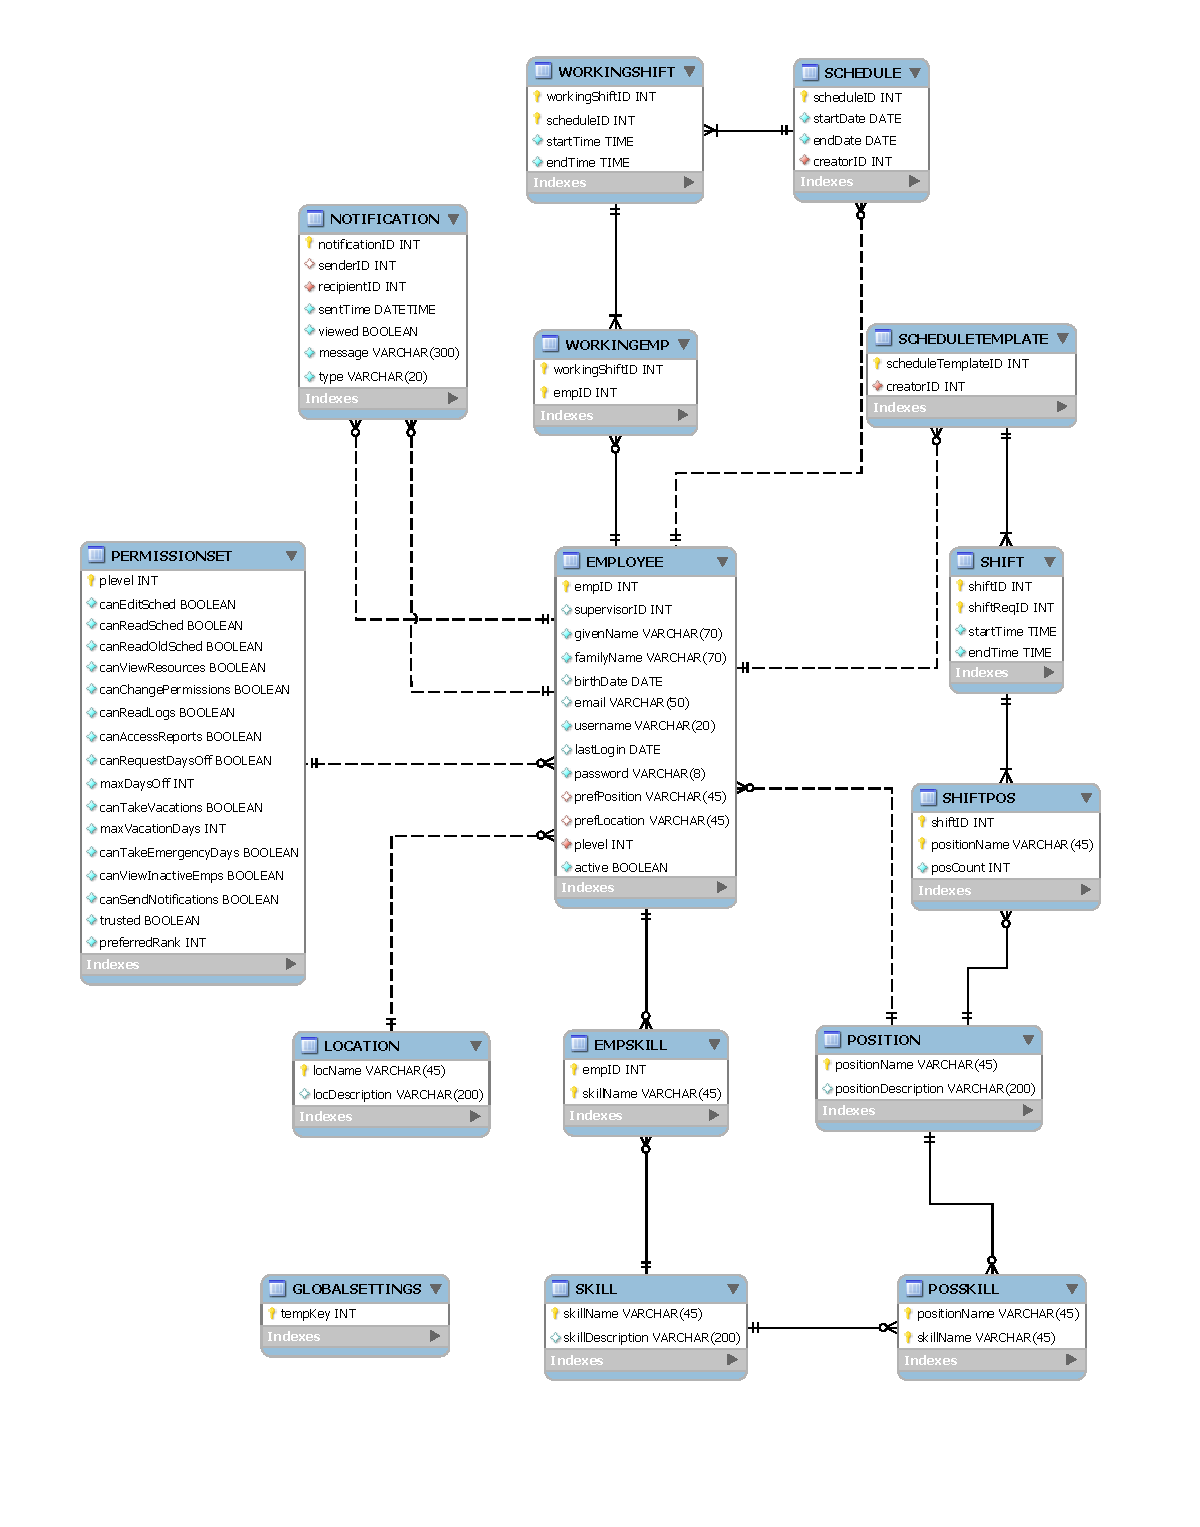
\includegraphics[scale=0.8,trim=25mm 00mm 25mm 20mm]{externals/InternalERD.pdf}
 \caption{\small
\textbf{Implementation ERD Diagram}}\label{fig:implemERD}
\end{figure}
}
\chapter{Expected Persistent Class Sizes}
\newpage
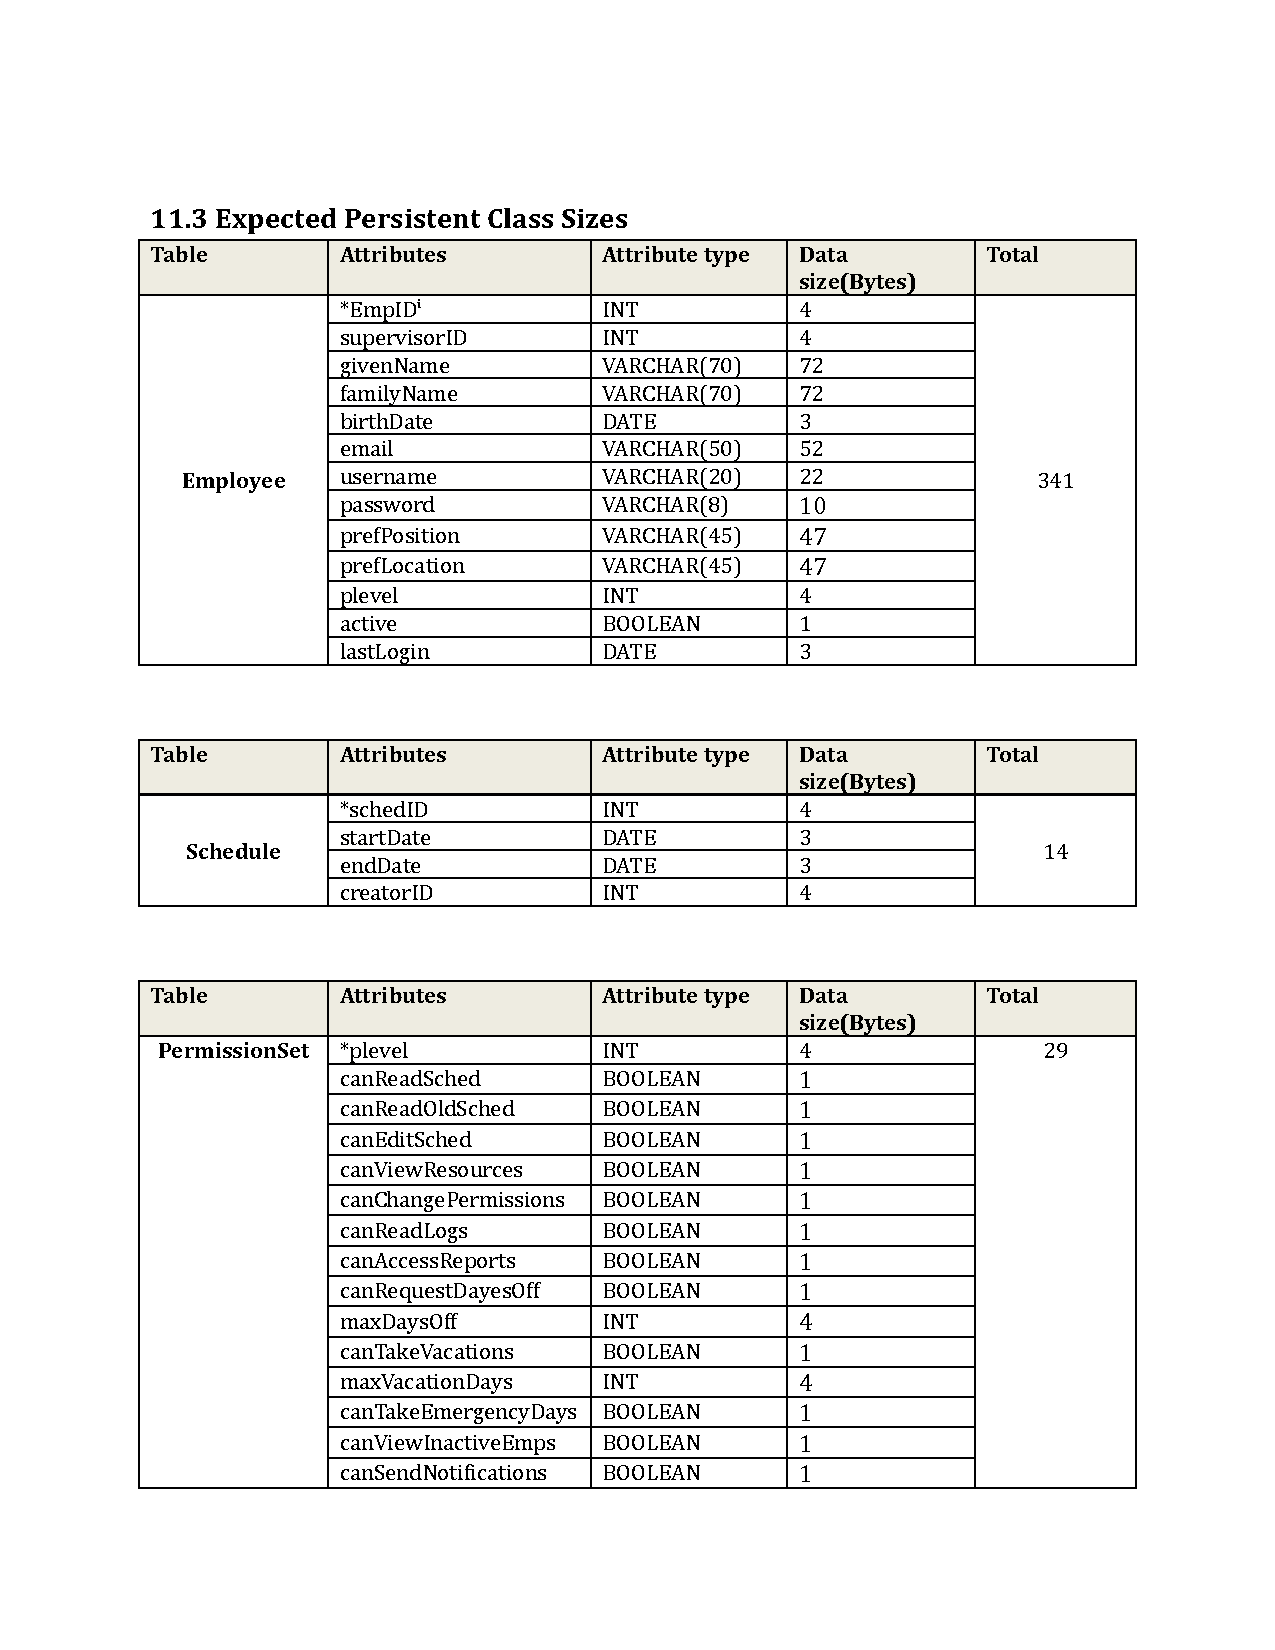
\includegraphics[trim=30mm 20mm 25mm 30mm]{ExternalFiles/DocumentStuff/datasizes1.pdf}

\newpage
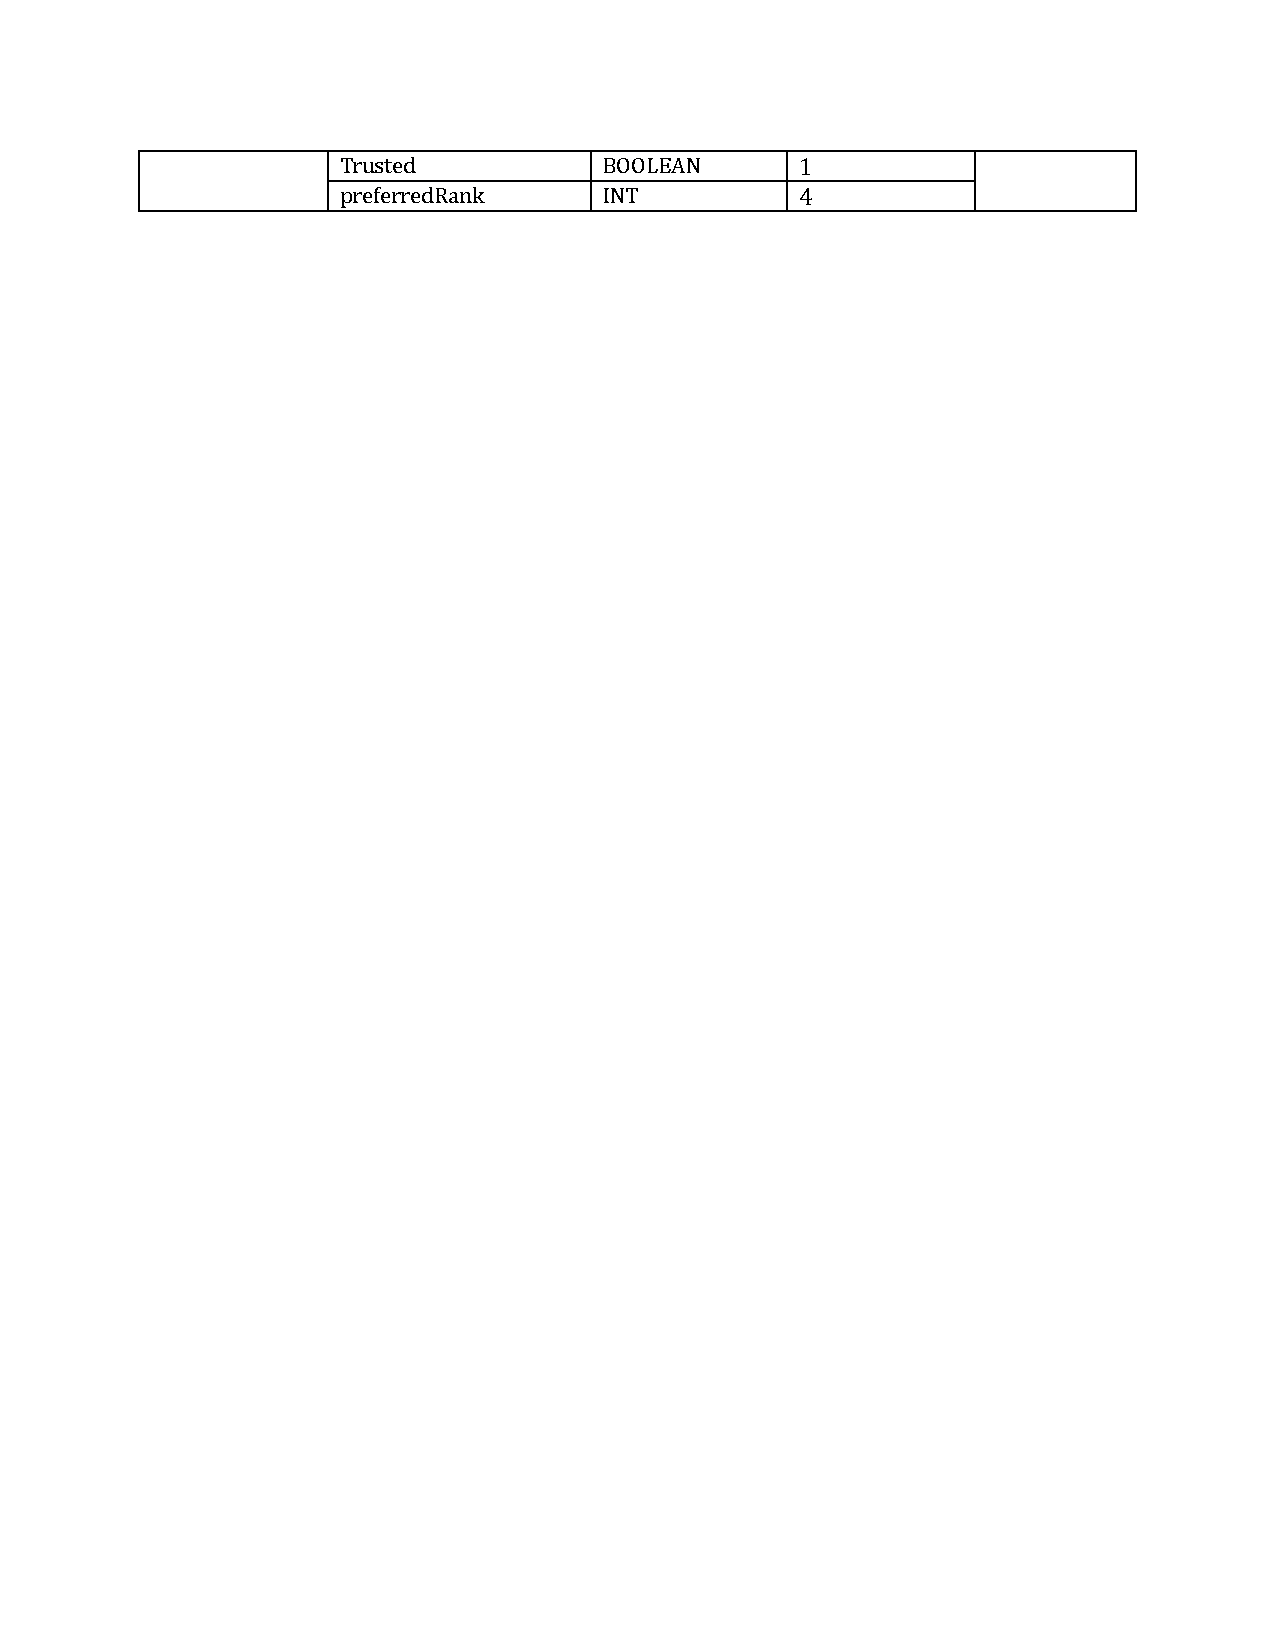
\includegraphics[trim=30mm 10mm 25mm 30mm]{ExternalFiles/DocumentStuff/datasizes2.pdf}

\newpage
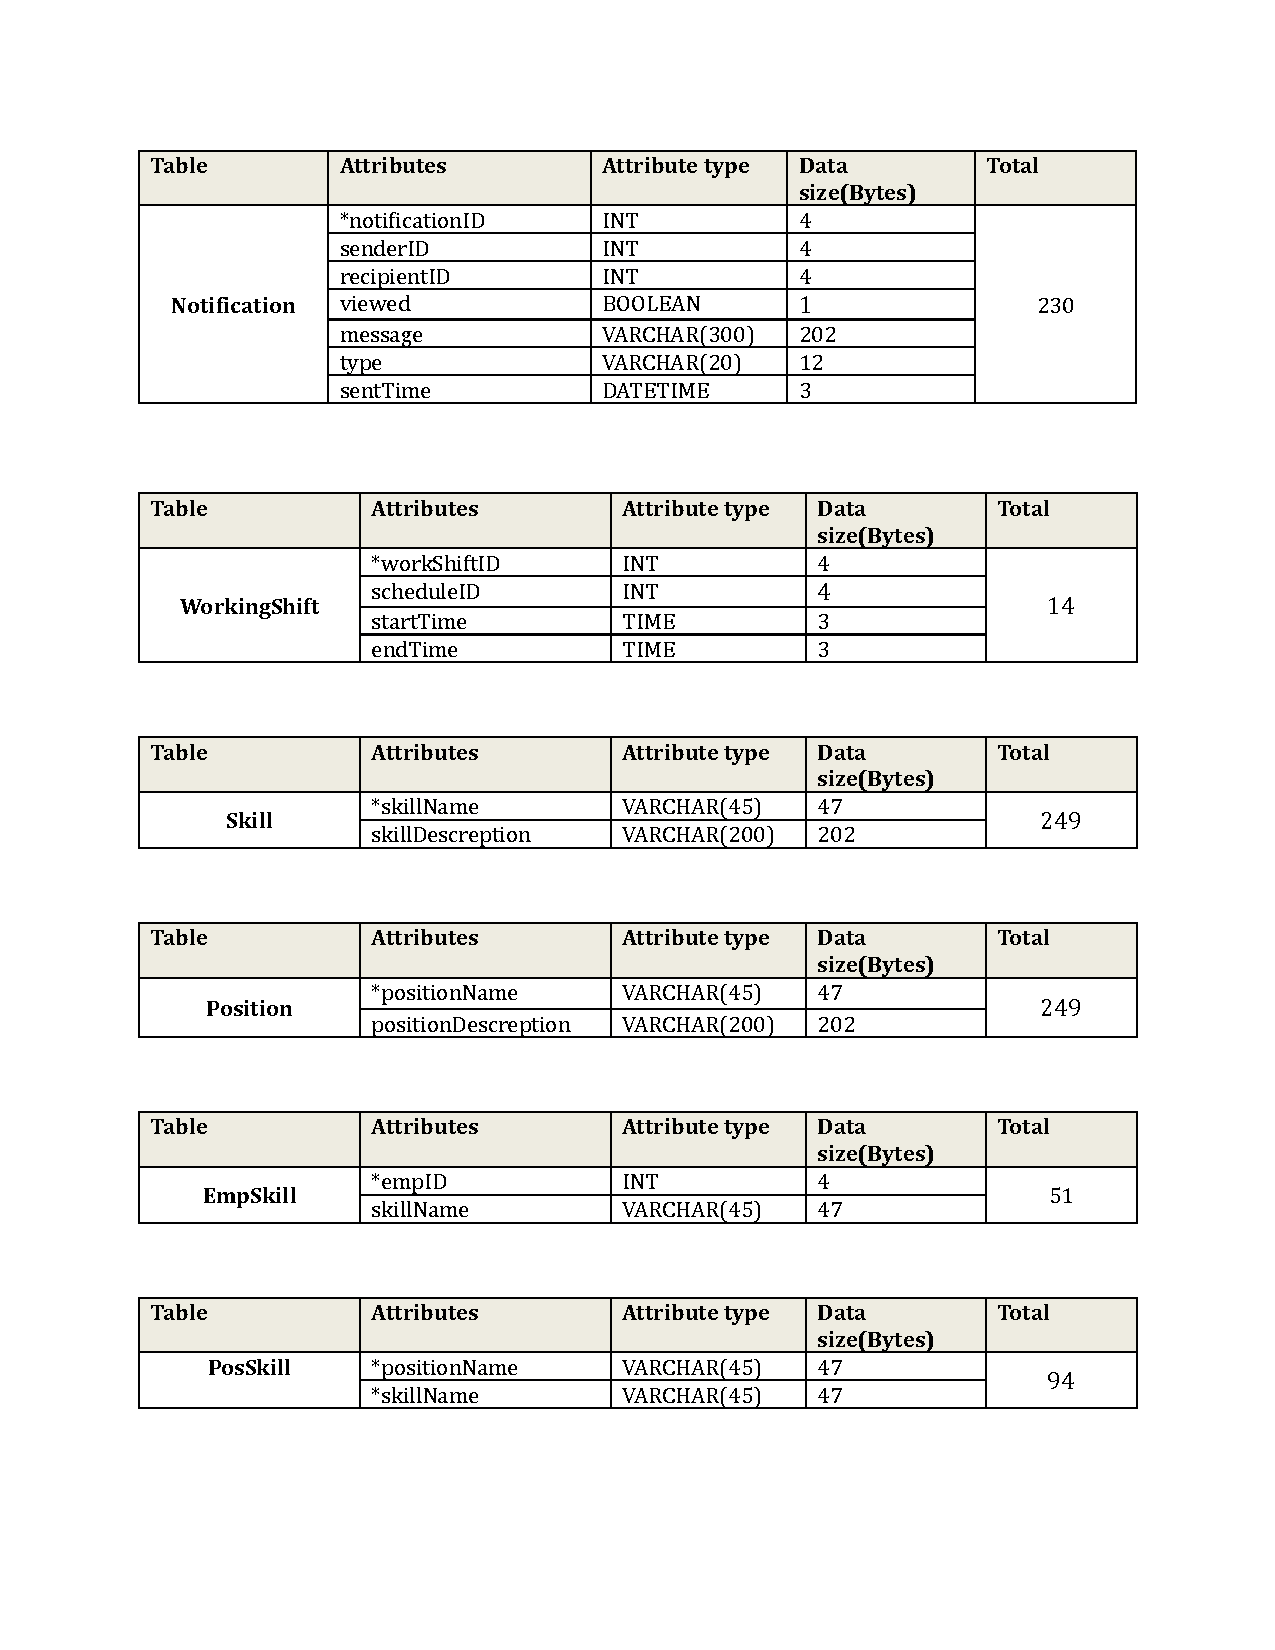
\includegraphics[trim=30mm 10mm 25mm 30mm]{ExternalFiles/DocumentStuff/datasizes3.pdf}

\newpage
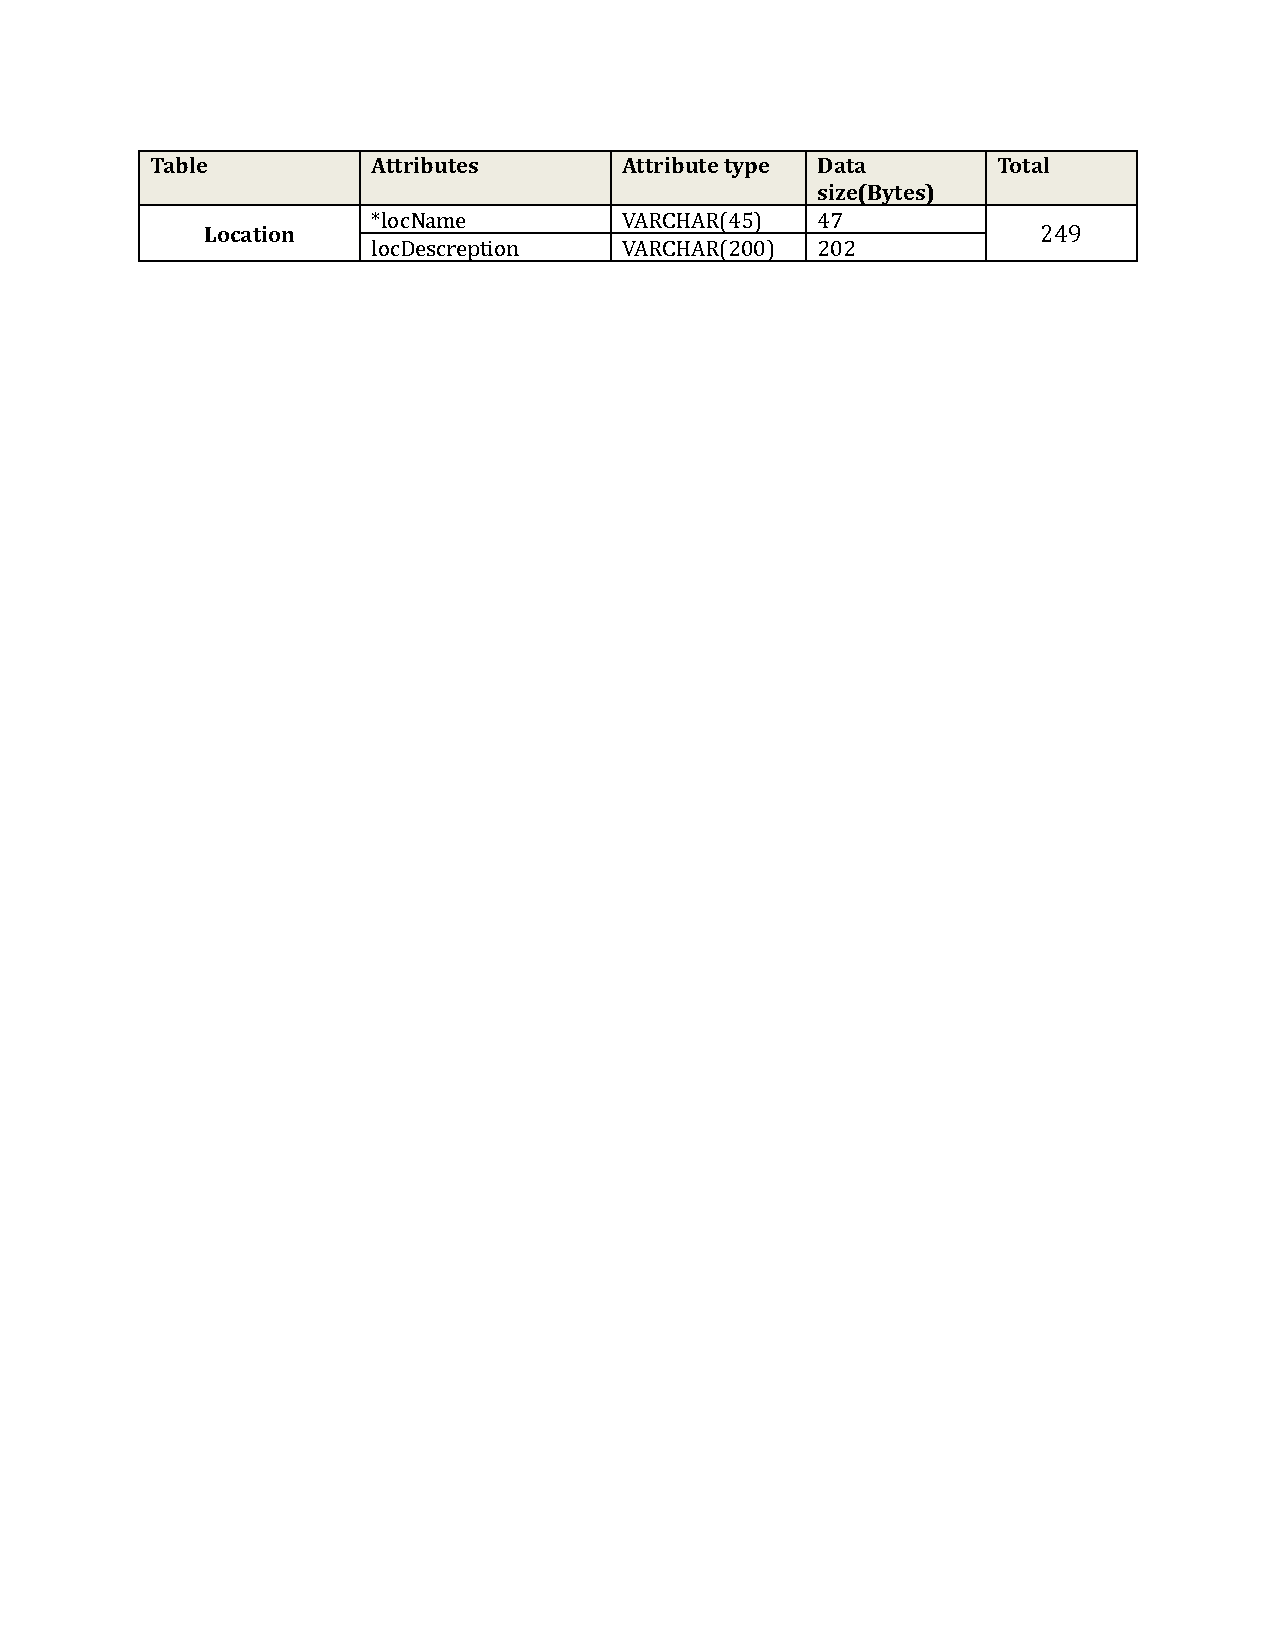
\includegraphics[trim=30mm 10mm 25mm 30mm]{ExternalFiles/DocumentStuff/datasizes4.pdf}

\newpage
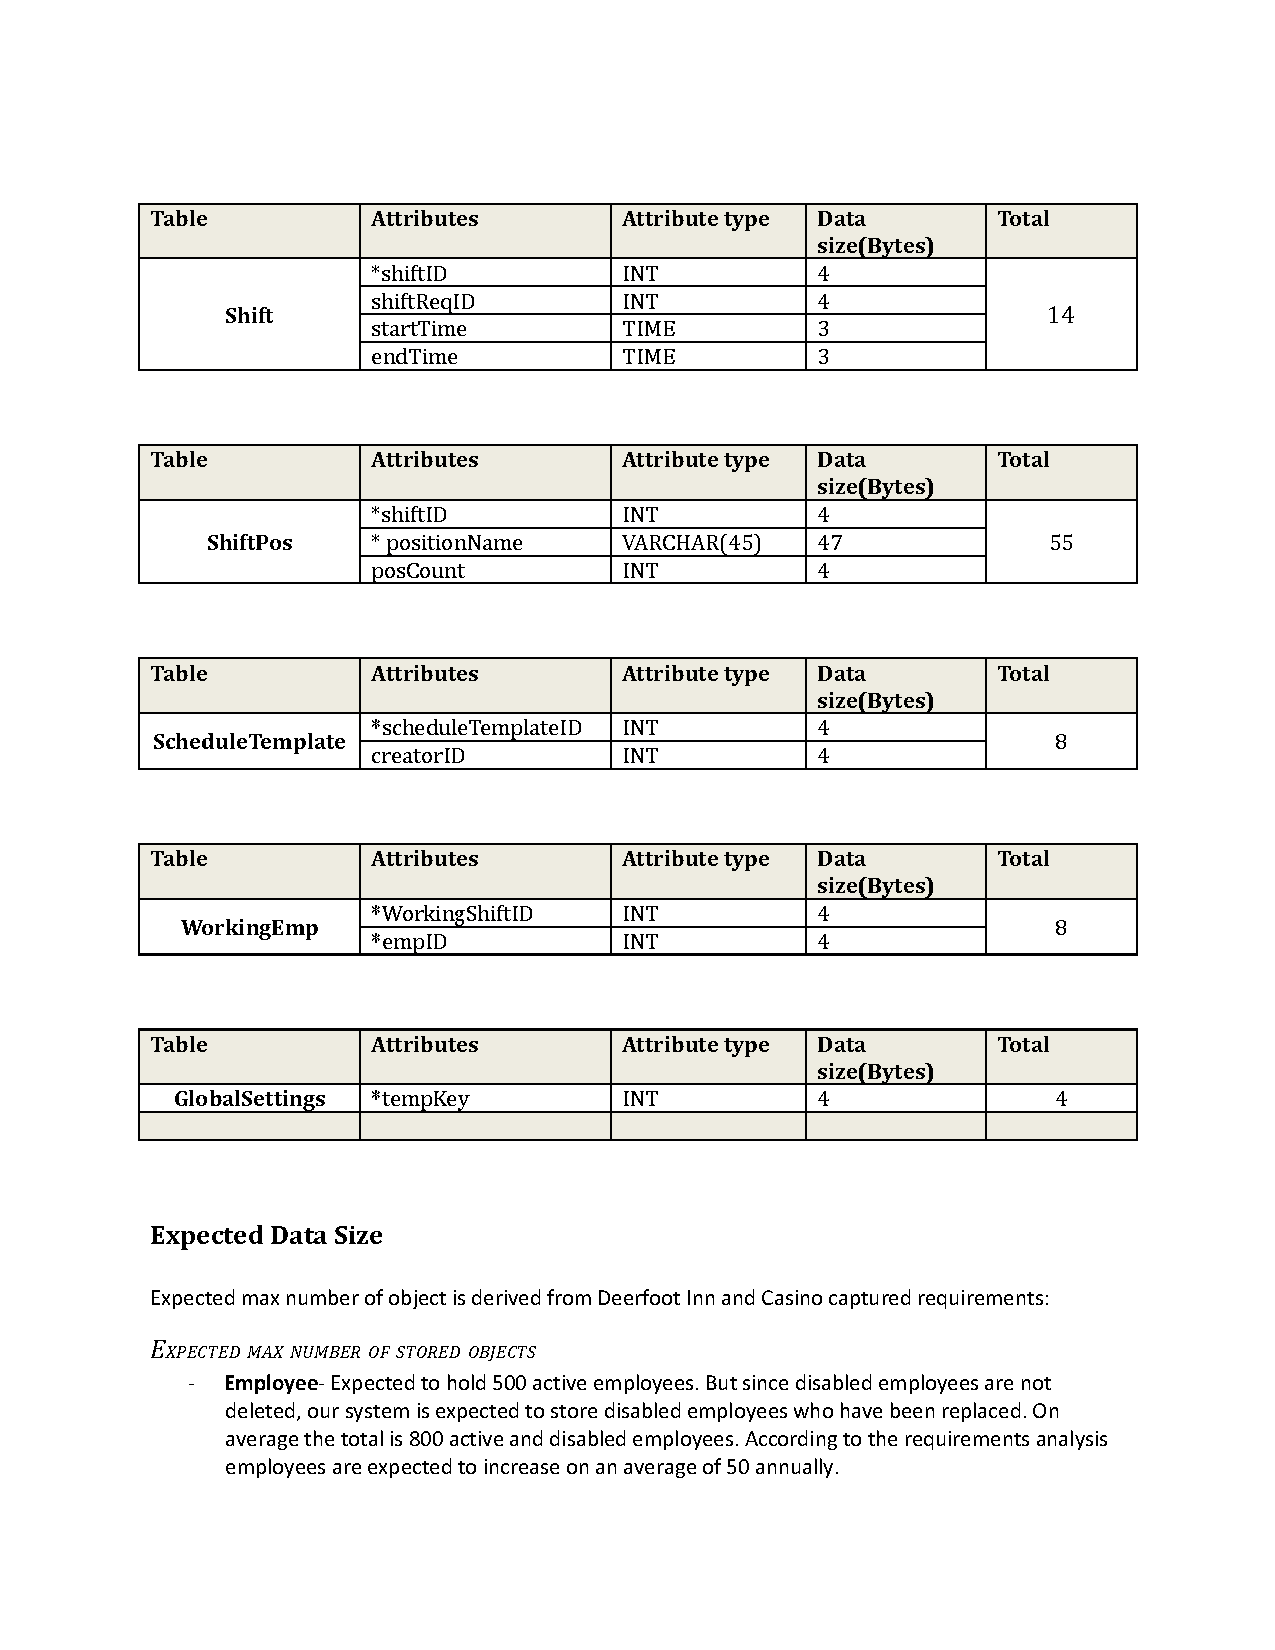
\includegraphics[trim=30mm 10mm 25mm 30mm]{ExternalFiles/DocumentStuff/datasizes5.pdf}

\newpage
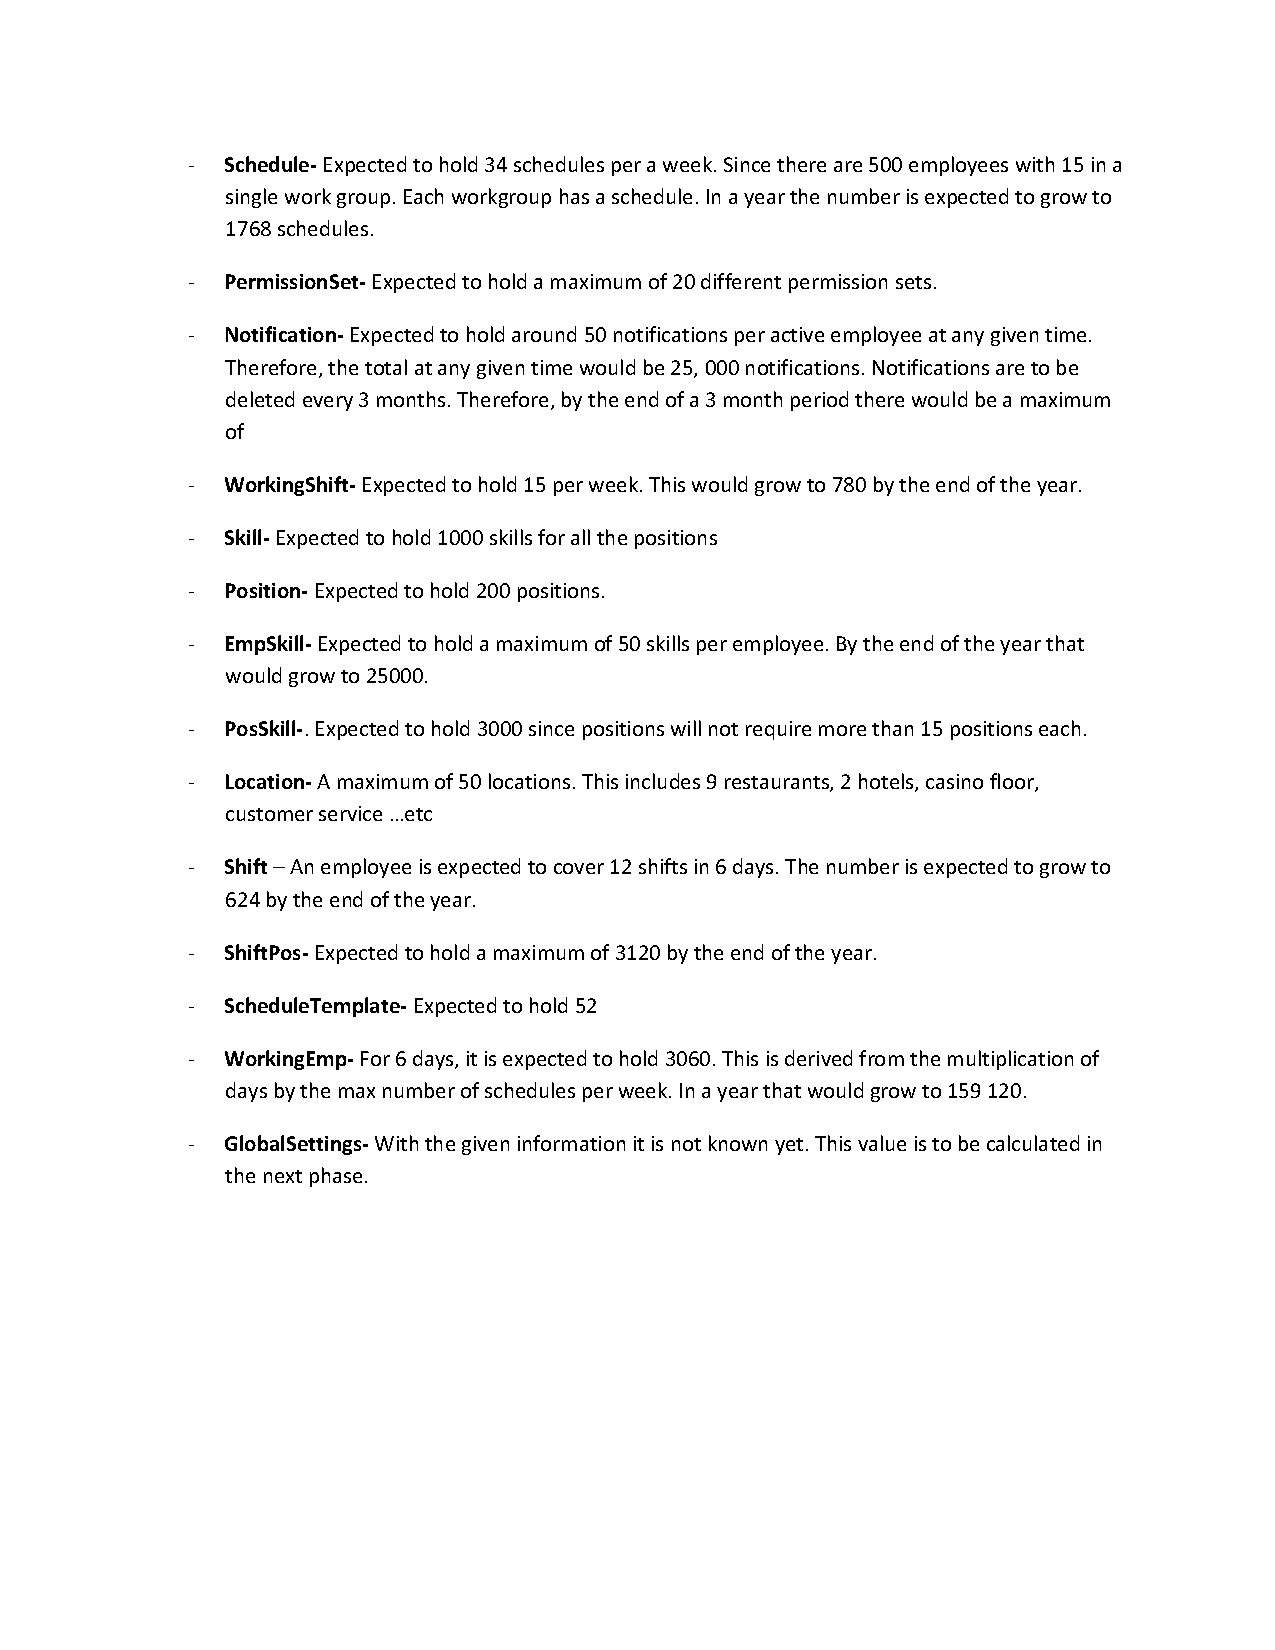
\includegraphics[trim=30mm 10mm 25mm 30mm]{ExternalFiles/DocumentStuff/datasizes6.pdf}

\newpage
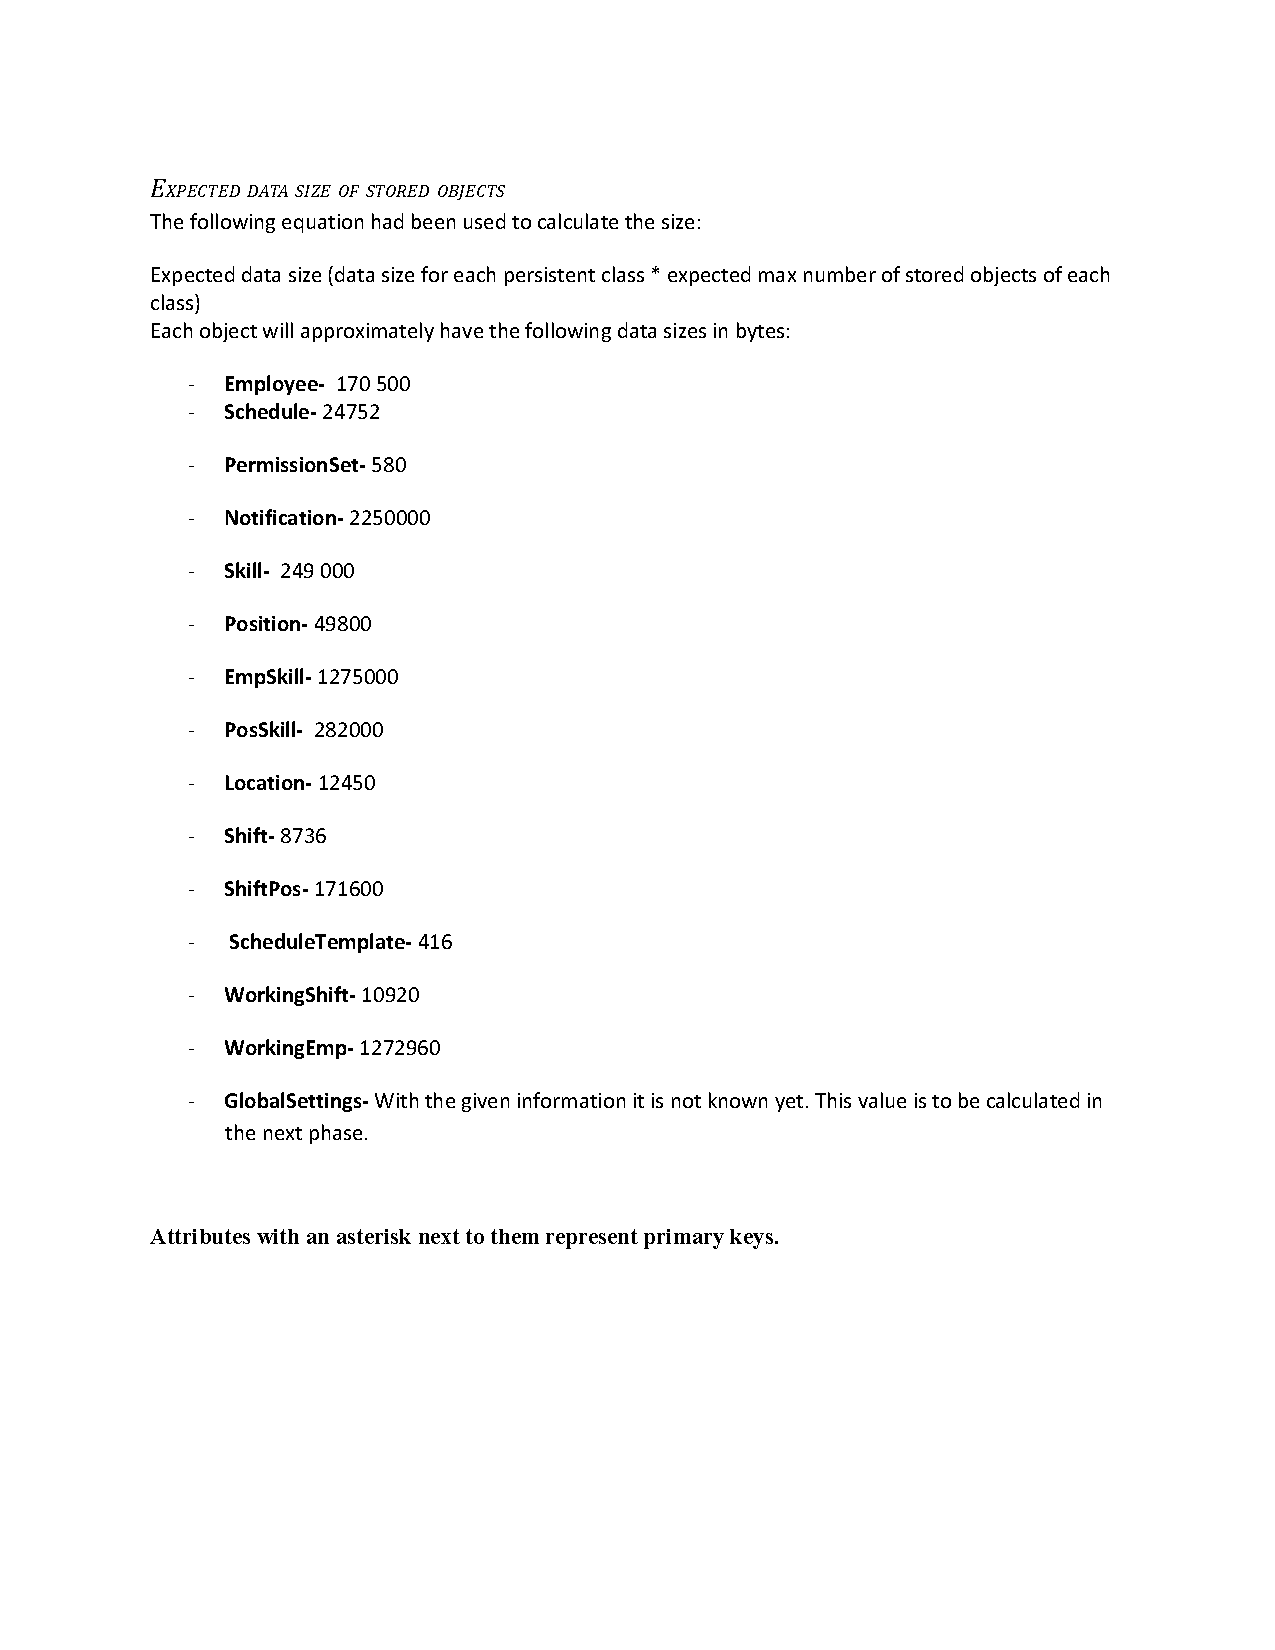
\includegraphics[trim=30mm 10mm 25mm 30mm]{ExternalFiles/DocumentStuff/datasizes7.pdf}

\chapter{Class Diagram}
\section{Interface, Persistence, Business and Problem Domain}
\newpage

\begin{figure}[interfaceClassDia]
 \centering
 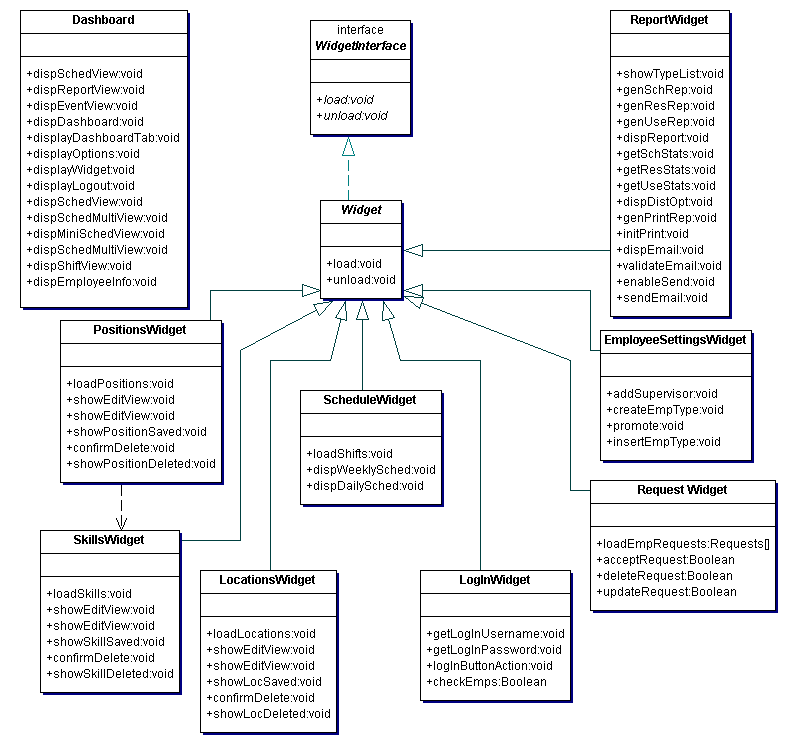
\includegraphics[scale=0.8]{externals/InterfaceClassDiagram.png}
 \caption{\small
\textbf{Interface Class Diagram}\newline This diagram shows the objects that make up the interface for WebAgenda\index{WebAgenda} and methods associated with them. }\label{fig:intclassdia}
\end{figure}
\newpage
\begin{figure}[persistdomainClassDia]
 \centering
 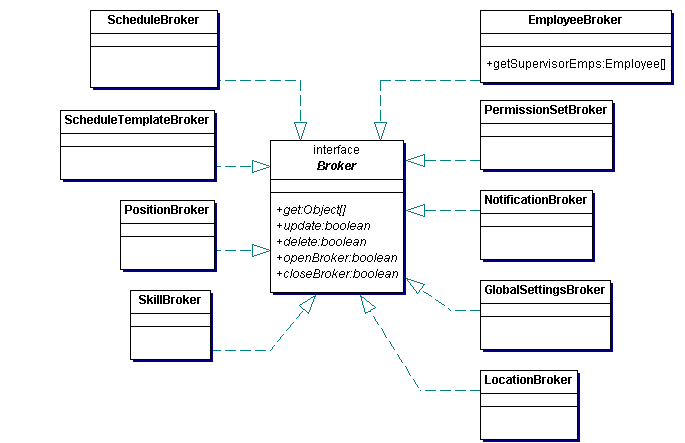
\includegraphics[scale=0.8]{externals/PersistenceClassDiagram.png}
 \caption{\small
\textbf{Persistence Class Diagram}\newline This diagram shows the objects that make up the persistence layer, the classes and objects that utilize backend or data objects}\label{fig:persclassdia}
\end{figure}
\newpage
\begin{figure}[applicationClassDia]
 \centering
 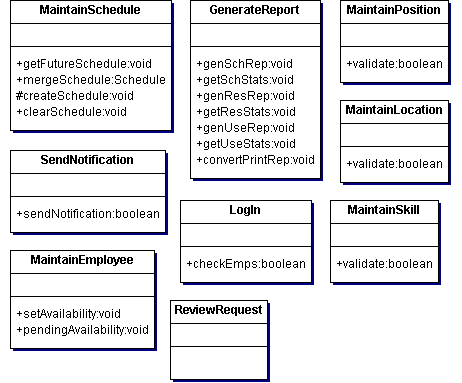
\includegraphics[scale=0.8]{externals/ApplicationClassDiagram.png}
 \caption{\small
\textbf{Application Class Diagram}\newline This diagram shows the objects that make up the application-side real world objects.\index{application}}\label{fig:pdclassdia}
\end{figure}
\newpage
\begin{figure}[businessClassDia]
 \centering
 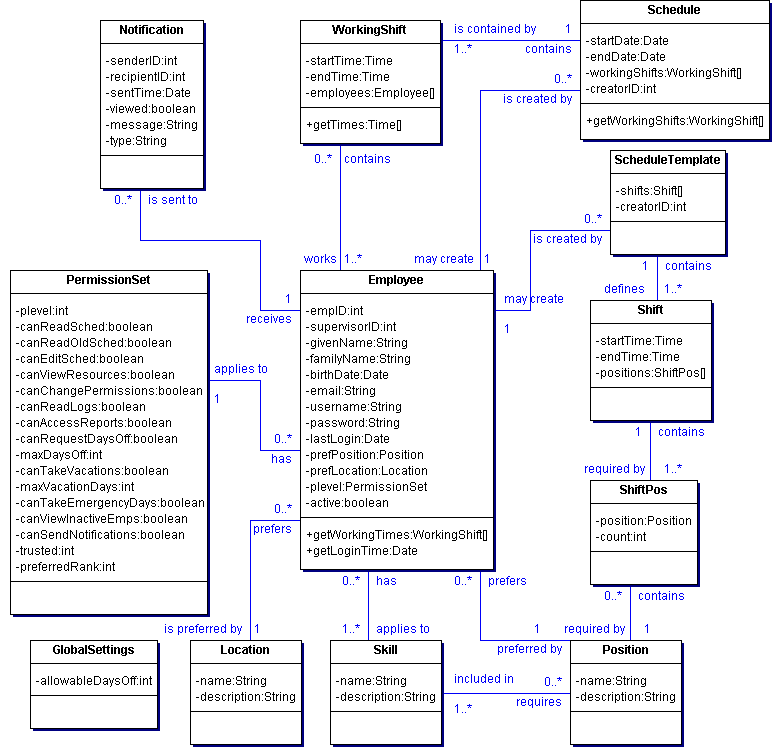
\includegraphics[scale=0.8]{externals/BusinessClassDiagram.png}
 \caption{\small
\textbf{Business Class Diagram}\newline Similar to the problem domain, this diagram displays the business classes. Business classes contain data that reflect real world objects that are used and modified in a business.}\label{fig:buisclassdia}
\end{figure}
\newpage


\clearpage
\chapter{Interaction Sequence Diagrams}
\newpage

\section{New Schedule Sequence Diagram}
\begin{figure}[hbp]
 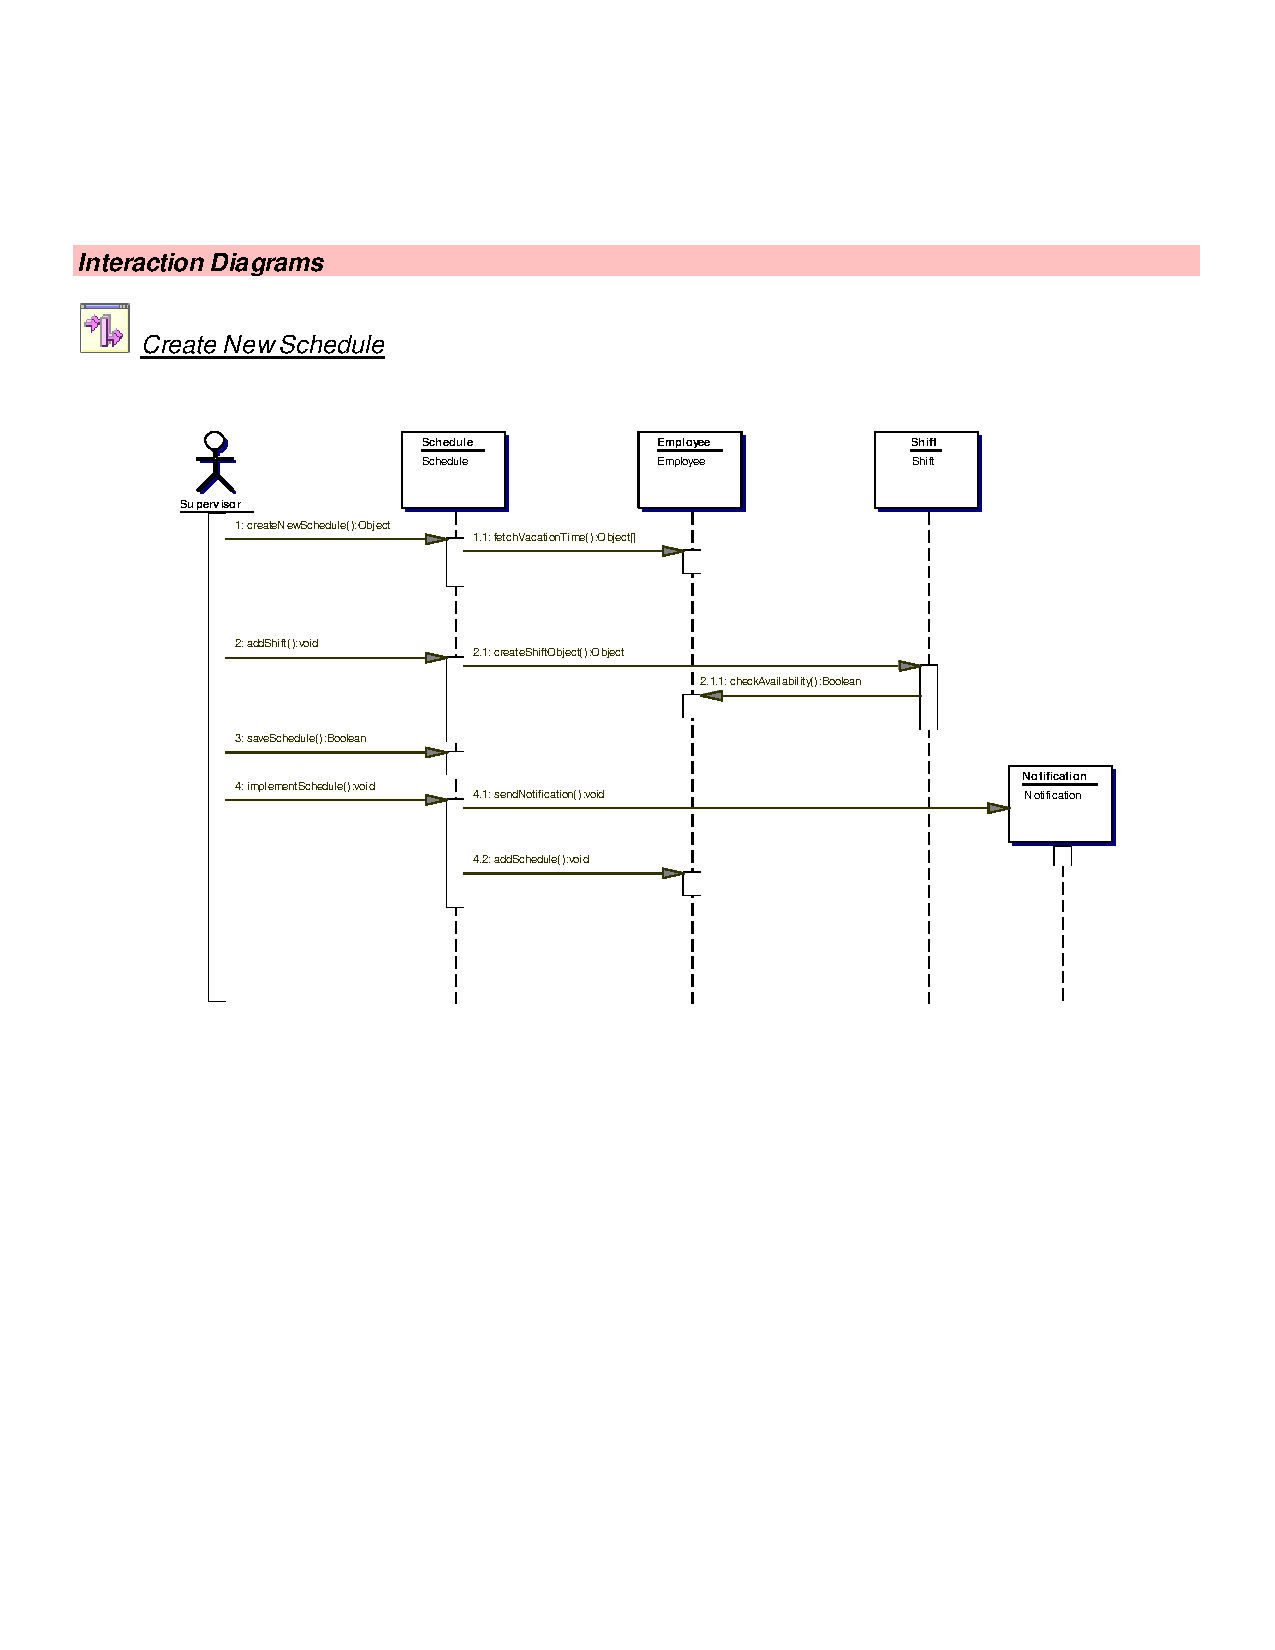
\includegraphics[trim=20mm 80mm 25mm 45mm]{diagrams/seq1.pdf}
 \caption{\small
\textbf{New \index{Schedule}Schedule Creation Sequence Diagram}\newline A representation of the proper sequence in creating a new schedule}\label{fig:seq1}
\end{figure}
\newpage
\section{Request Shift Change Sequence Diagram}
\begin{figure}[hbp]
 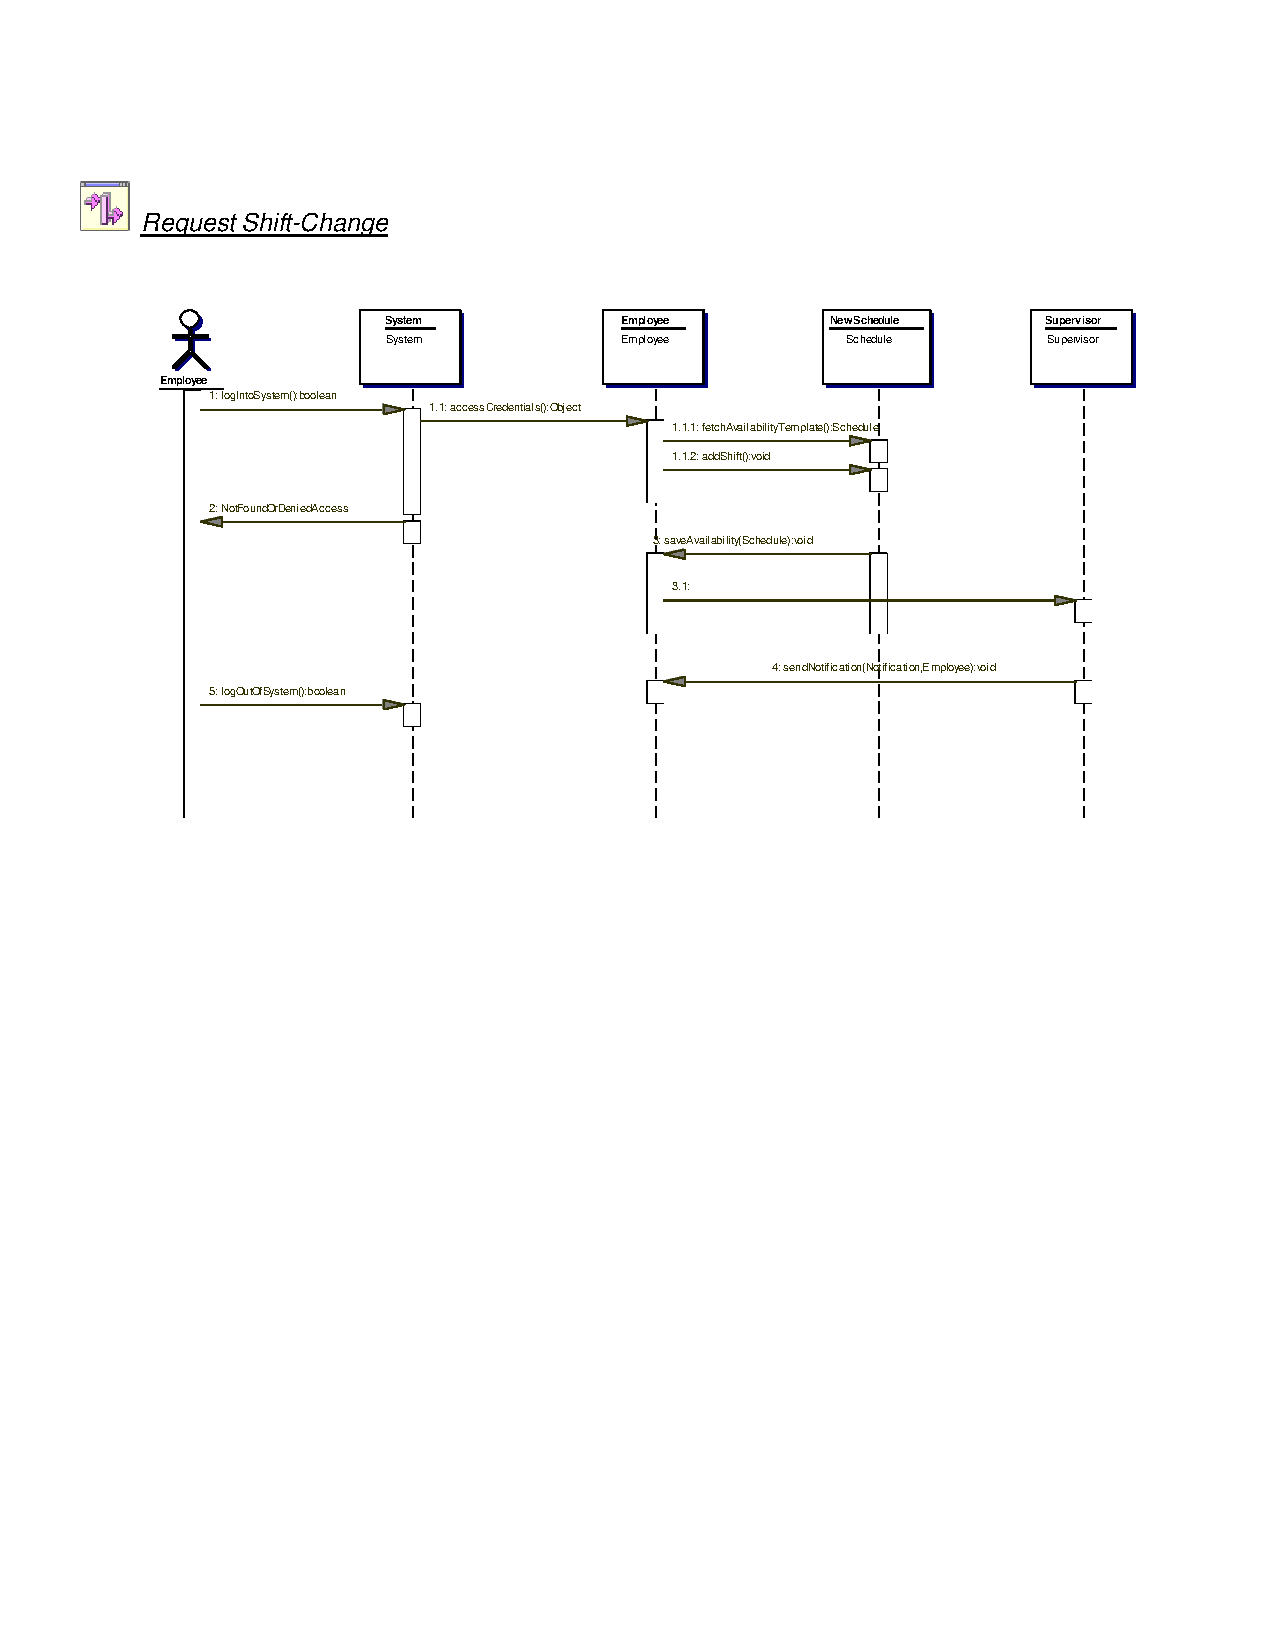
\includegraphics[trim=20mm 90mm 25mm 35mm]{diagrams/seq2.pdf}
 \caption{\small
\textbf{Request Shift Change Sequence Diagram}\newline A representation of the proper sequence in requesting a shift change}\label{fig:seq2}
\end{figure}
\newpage
\section{Viewing Schedule Sequence Diagram}
\begin{figure}[hbp]
 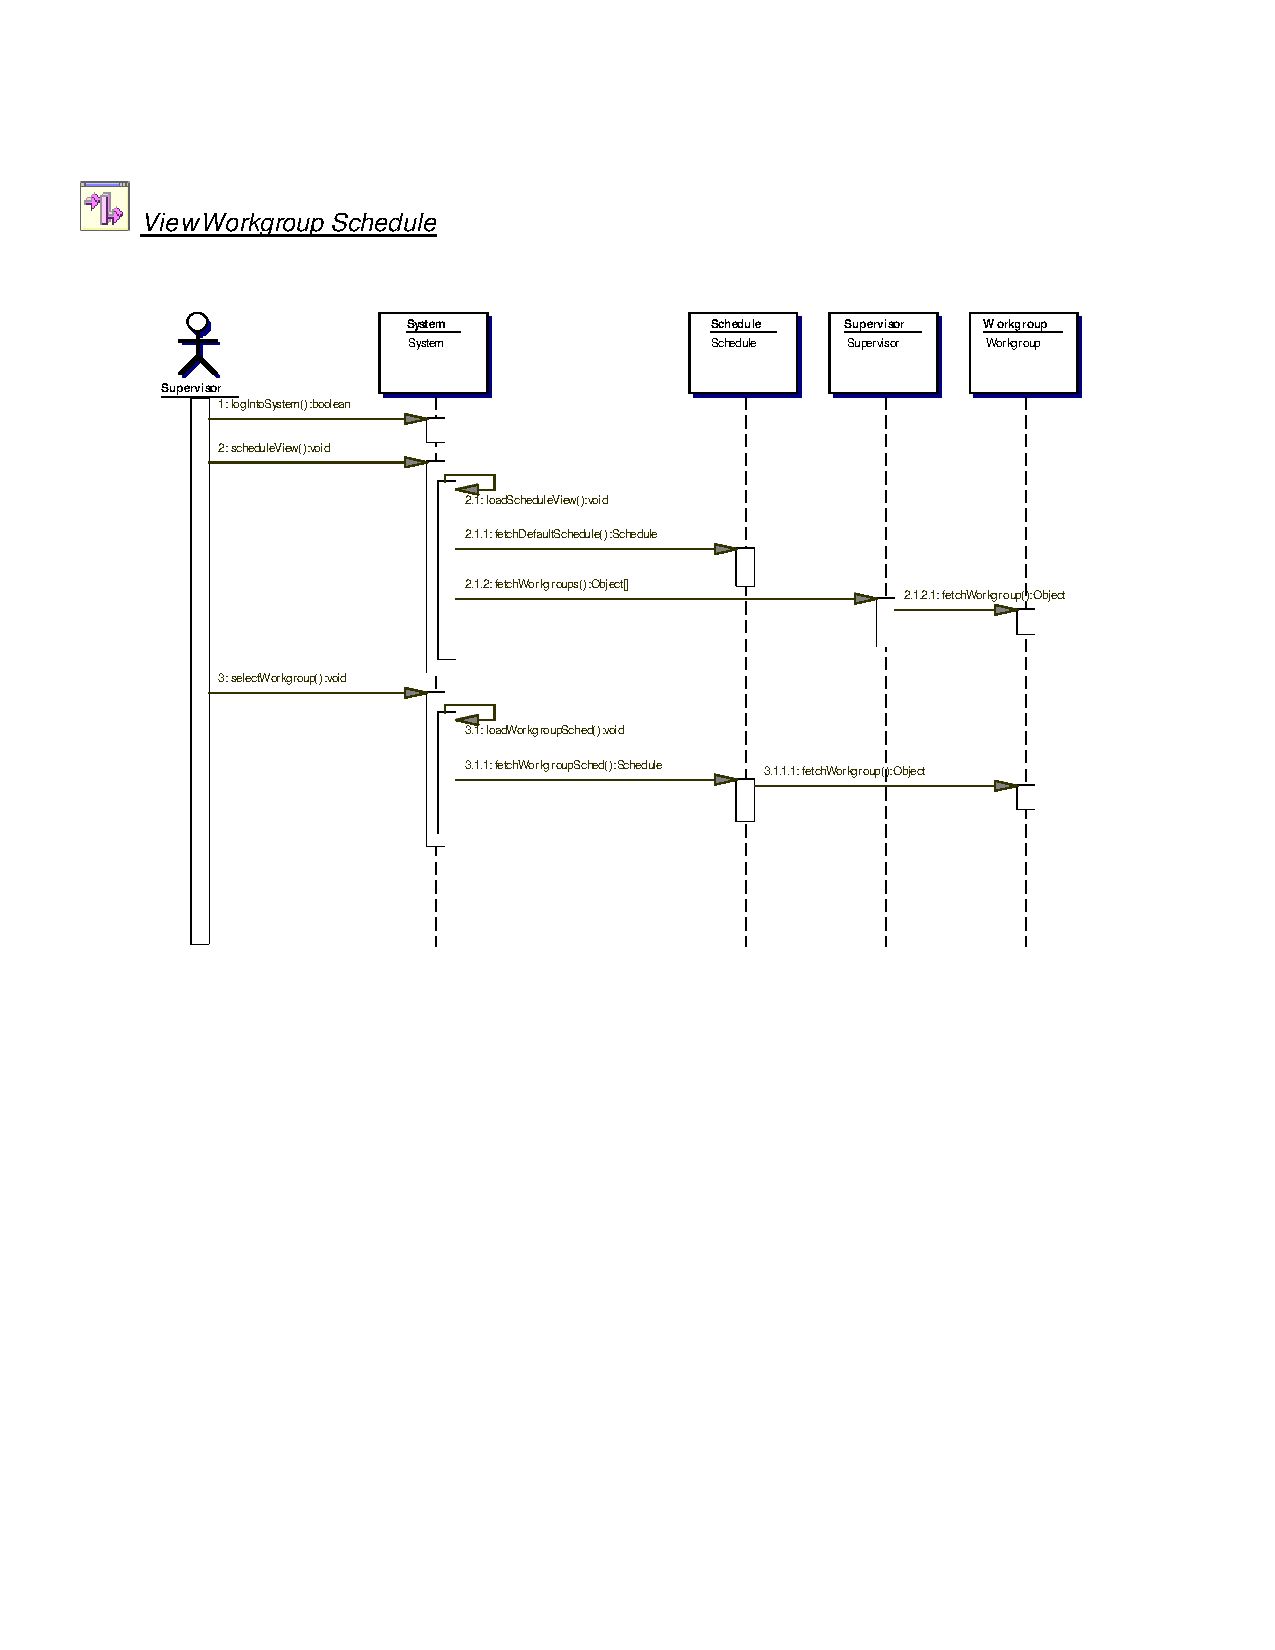
\includegraphics[trim=20mm 90mm 25mm 35mm]{diagrams/seq3.pdf}
 \caption{\small
\textbf{Viewing Schedule Sequence Diagram}\newline A representation of the proper sequence for viewing a schedule}\label{fig:seq3}
\end{figure}
\newpage
\section{Book Days Off Sequence Diagram}
\begin{figure}[hbp]
 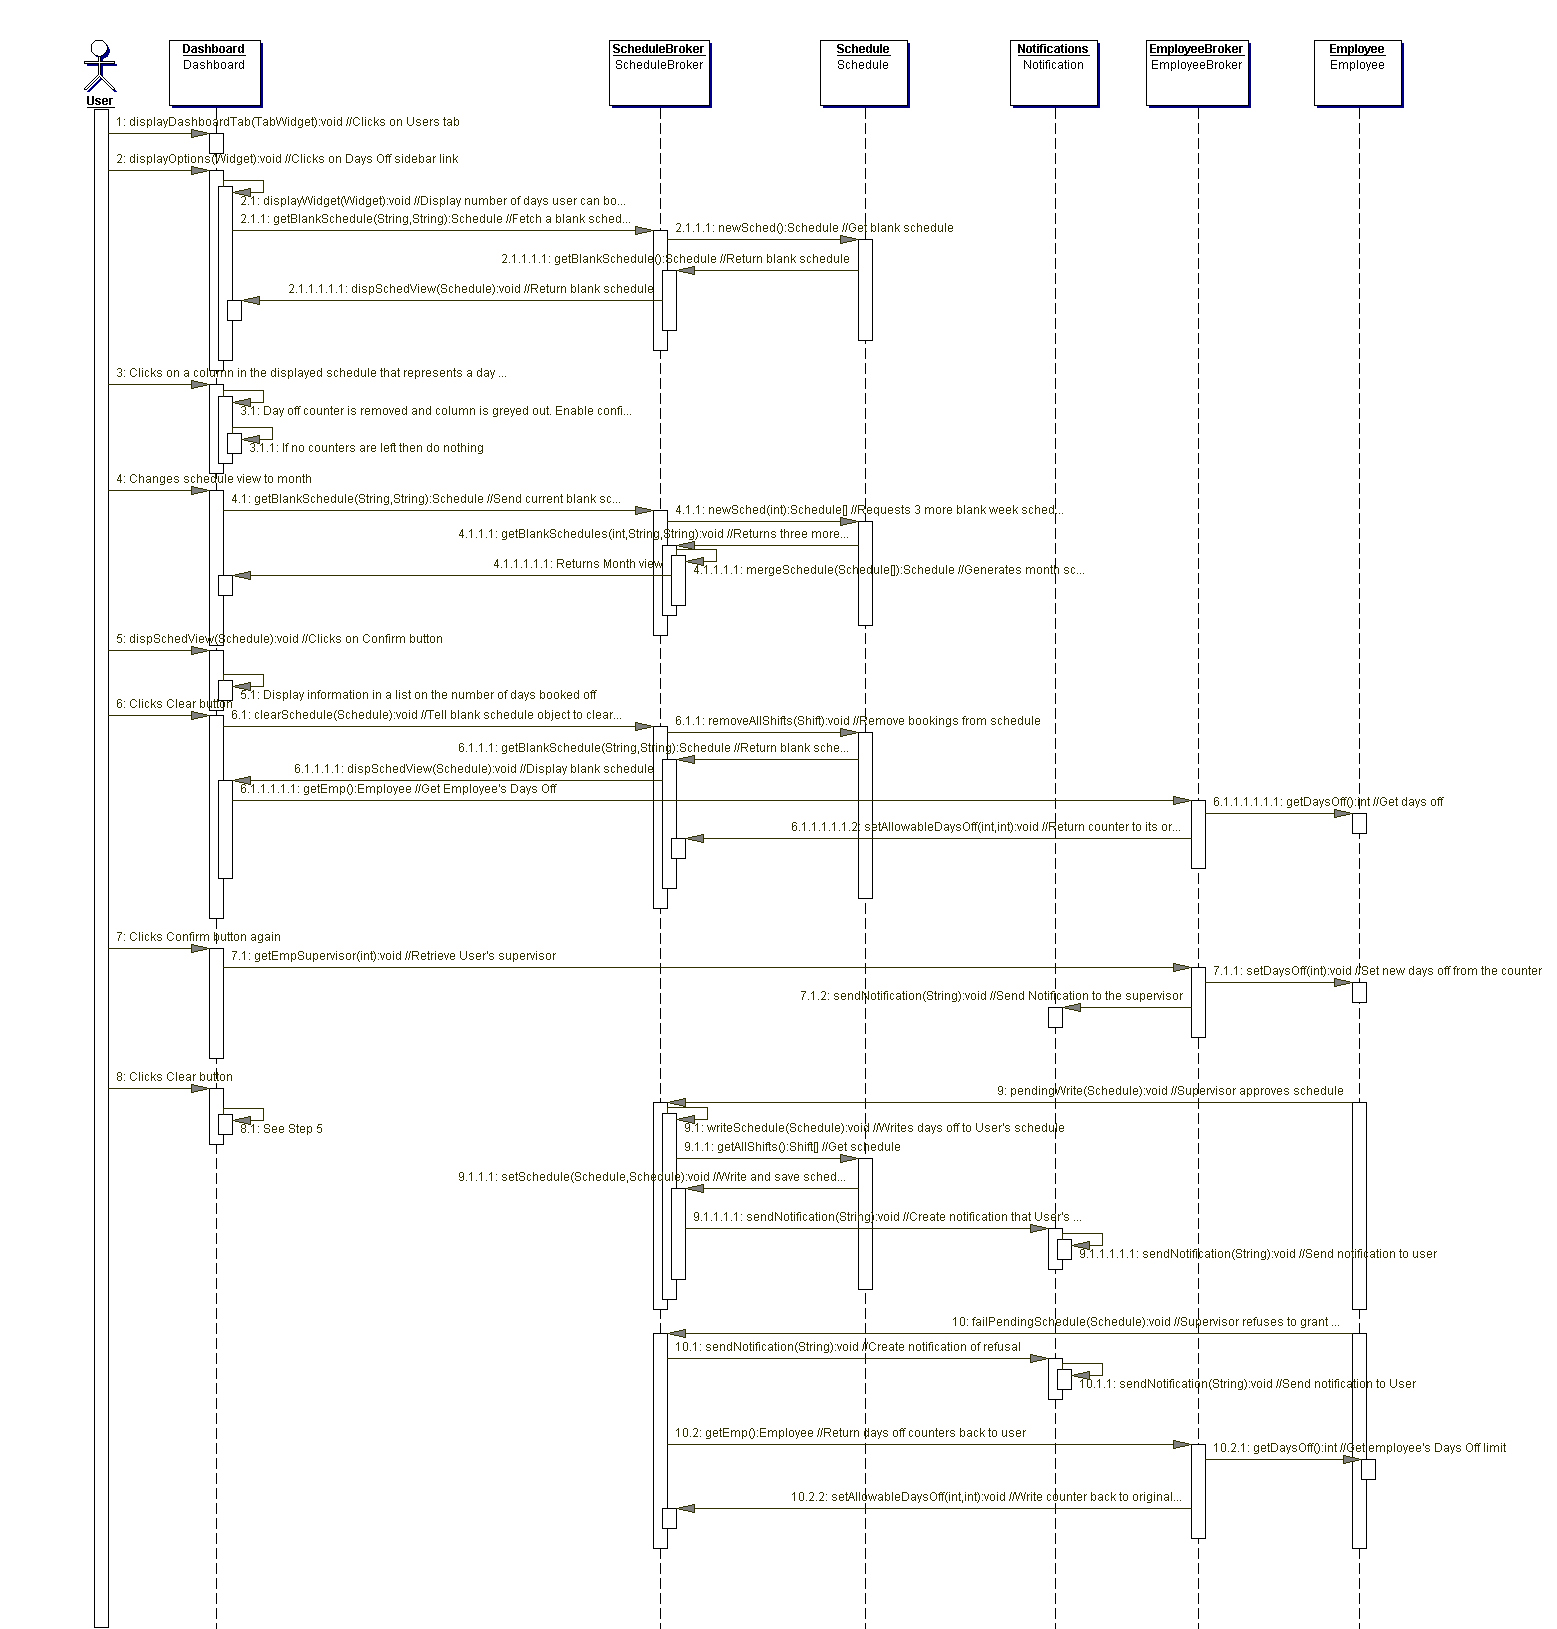
\includegraphics[scale=0.3]{diagrams/seqBookDaysOff.png}
 \caption{\small
\textbf{Book Days Off Sequence Diagram}\newline A representation of the proper sequence for booking days off}\label{fig:seqBookDaysOff}
\end{figure}
\newpage
\section{Administrative Schedule Viewing Sequence Diagram}
\begin{figure}[hbp]
 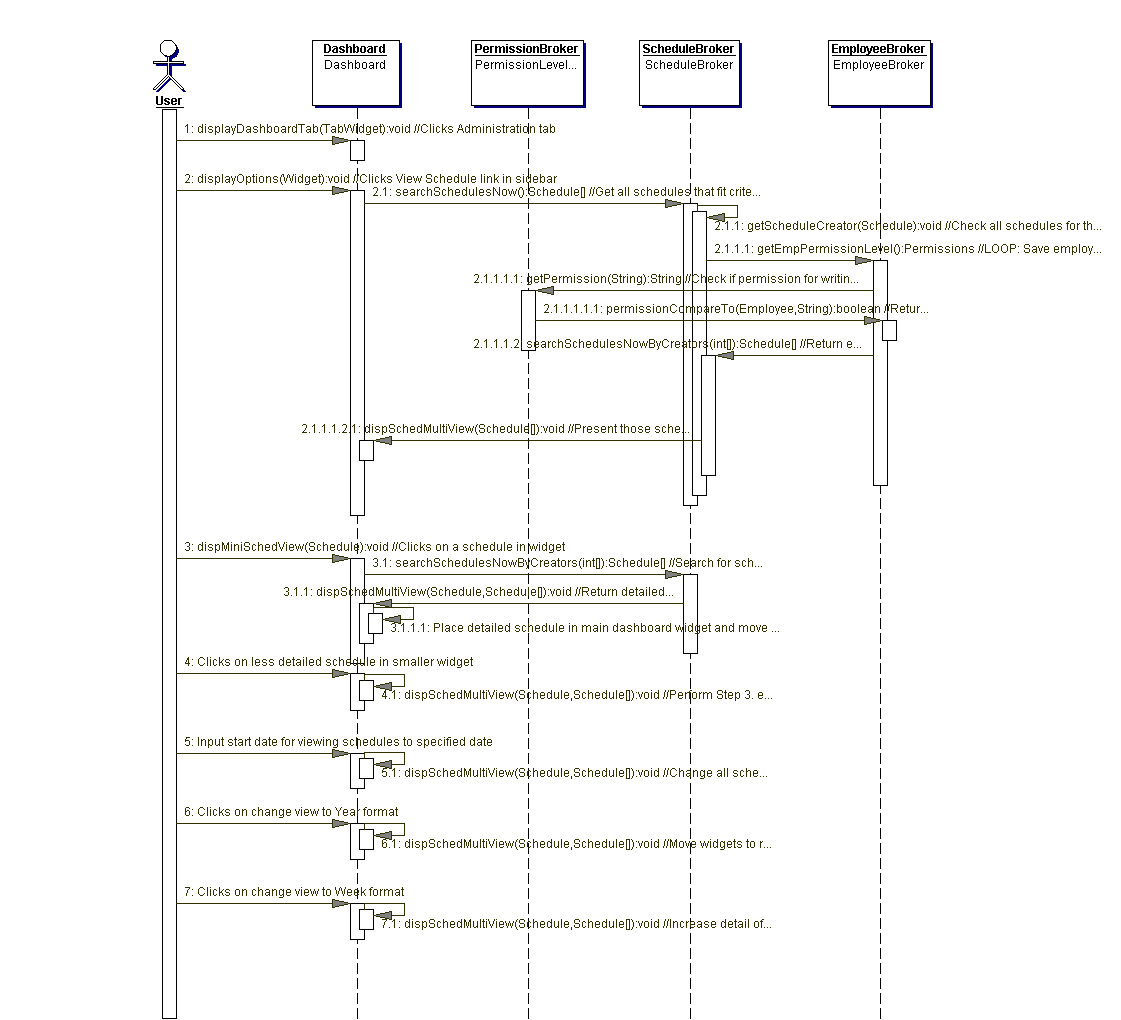
\includegraphics[scale=0.5]{diagrams/seqManagerViewScheds.png}
 \caption{\small
\textbf{Administrative Schedule Viewing Sequence Diagram}\newline A representation of the proper sequence for a manager or authoritative employee to view multiple schedules}\label{fig:seqManagerView}
\end{figure}
\newpage
\begin{figure}[hbp]
 \section{Request Shift Change Sequence Diagram}
 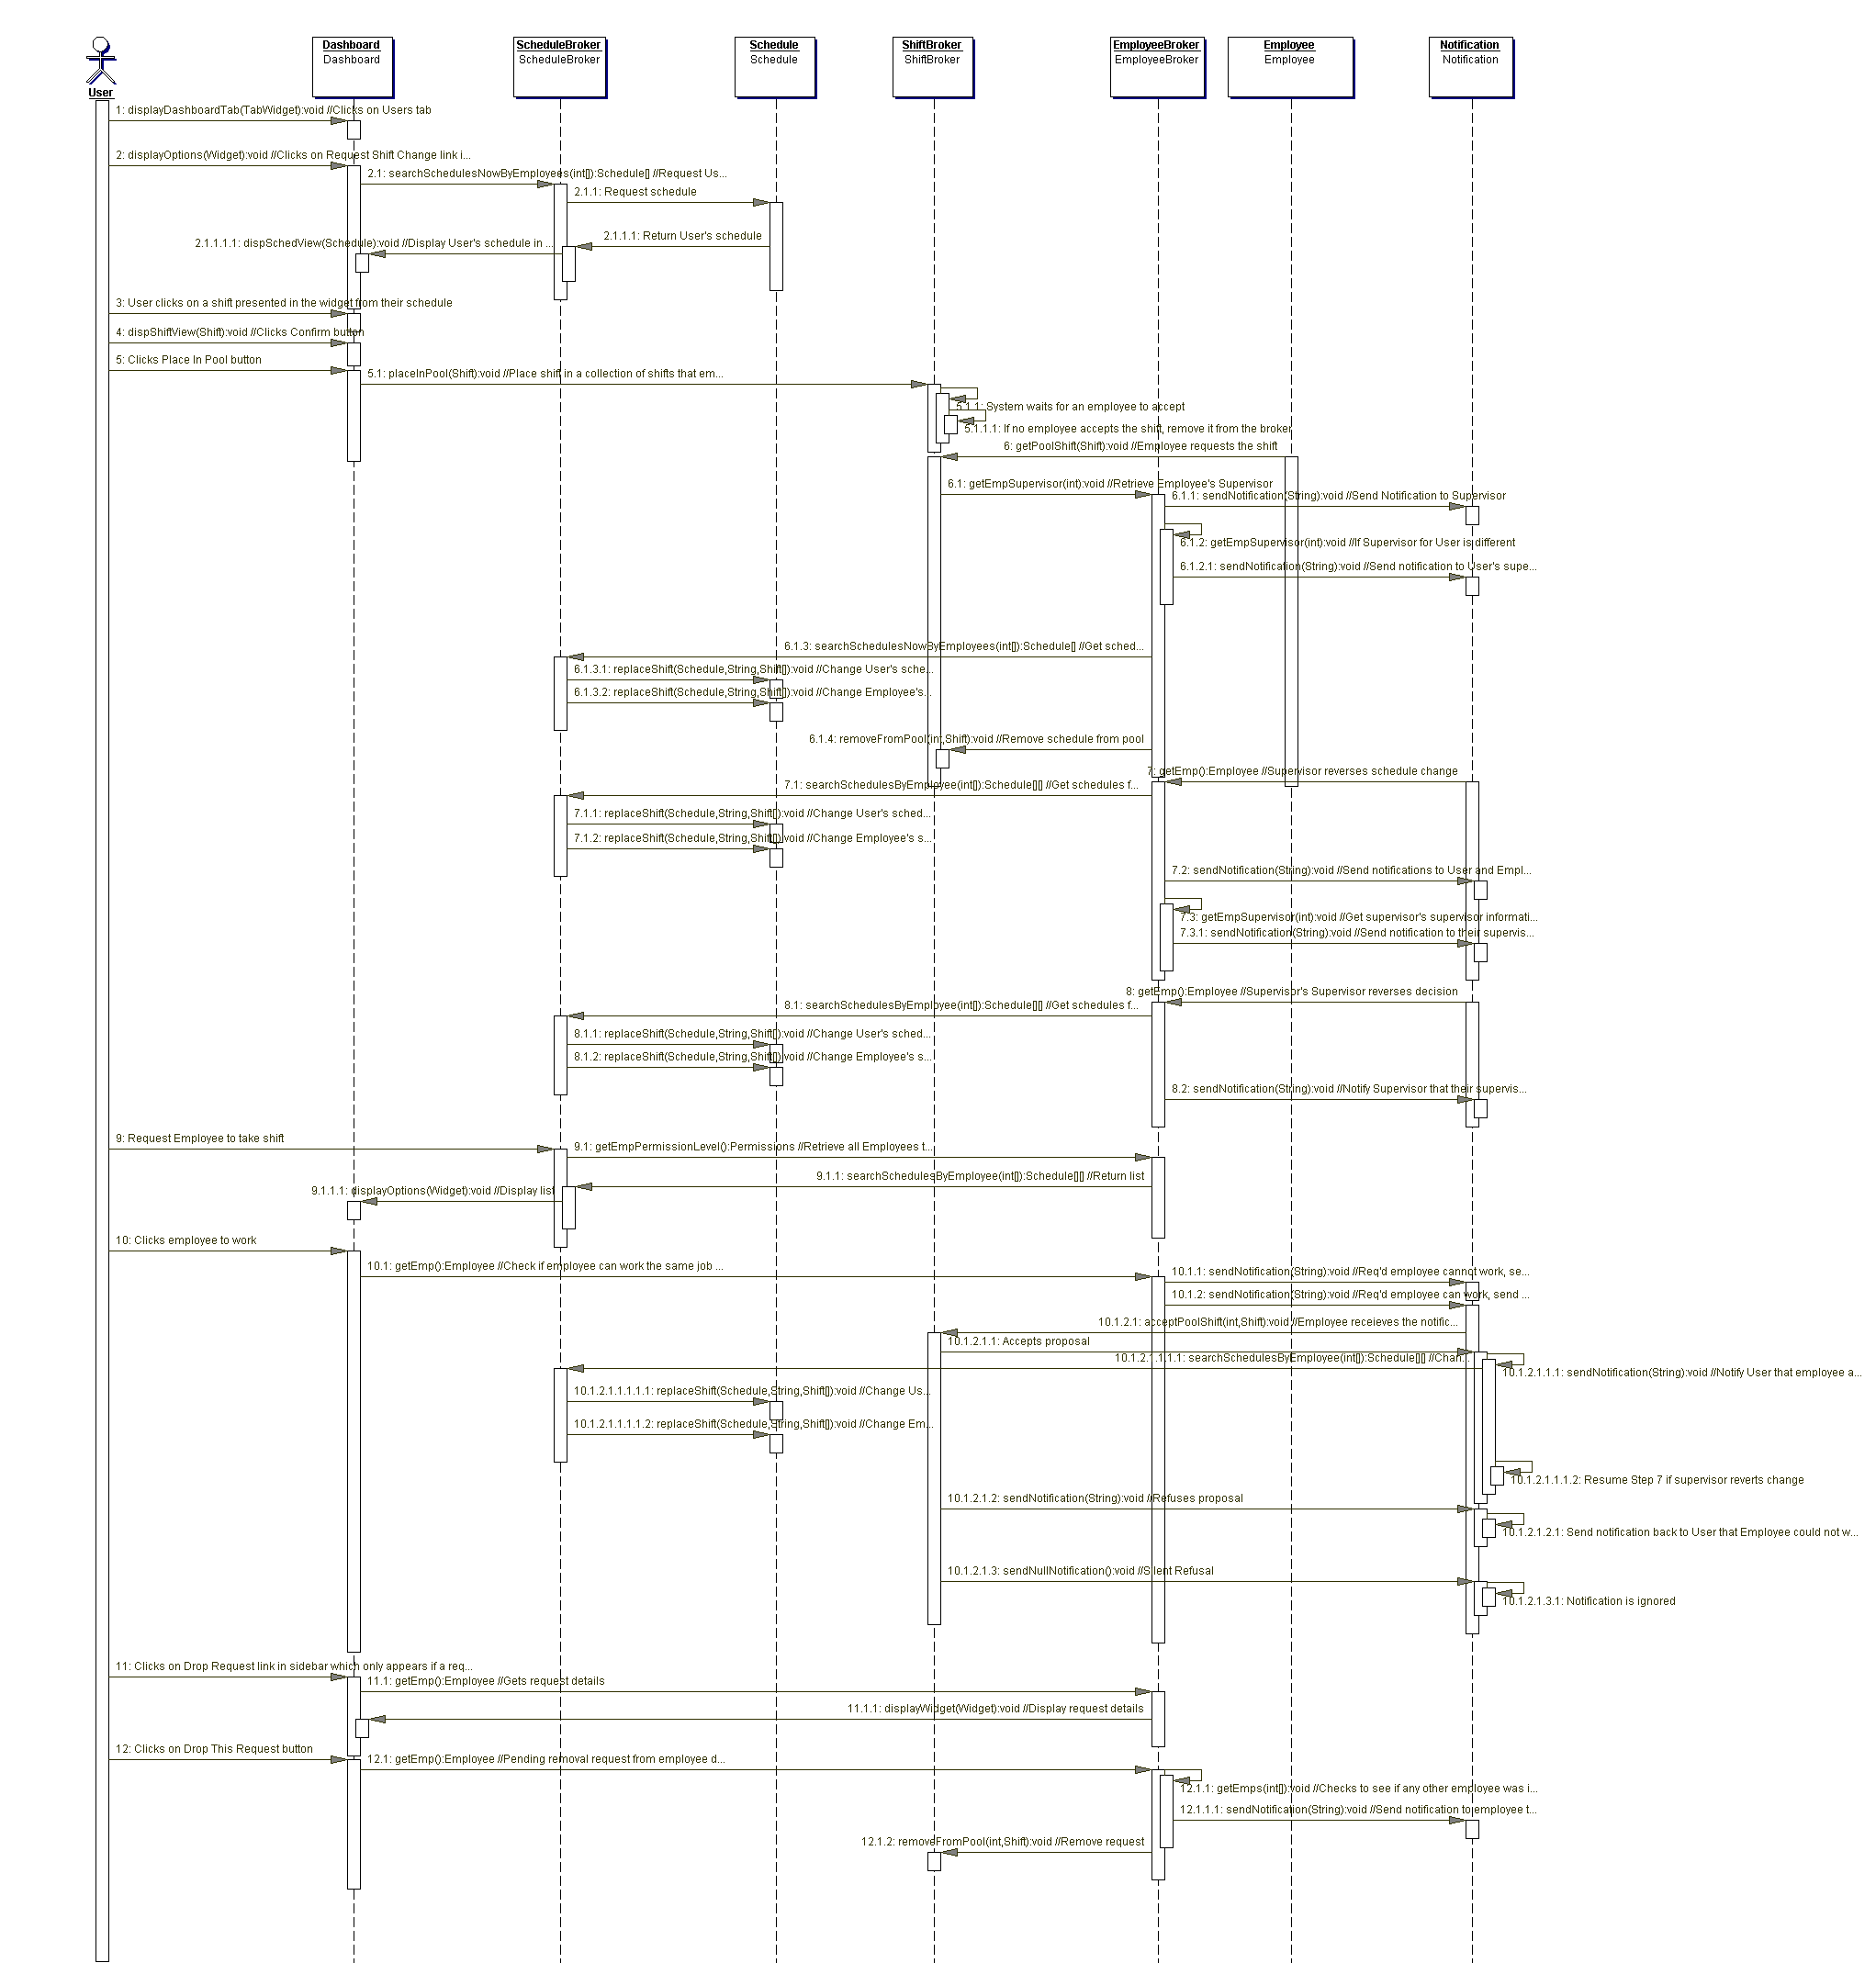
\includegraphics[scale=0.28]{diagrams/seqRequestShiftChange.png}
 \caption{\small
\textbf{Request Shift Change Sequence Diagram}\newline A representation of the proper sequence for changing a shift with another employee}\label{fig:seqRequestShiftChange}
\end{figure}
\newpage
\begin{figure}[hbp]
 \section{Update Availability Sequence Diagram}
 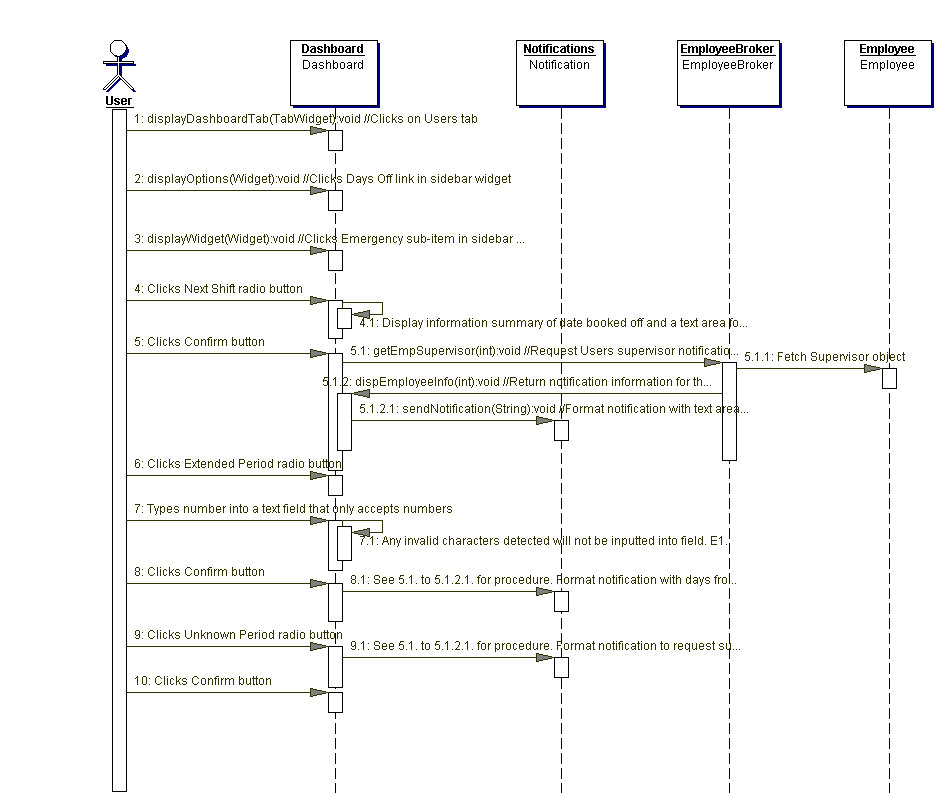
\includegraphics[scale=0.65]{diagrams/seqUpdateAvailability.png}
 \caption{\small
\textbf{Update Availability Sequence Diagram}\newline A representation of the proper sequence for updating an Employee`s availability}\label{fig:seqUpdateAvailability}
\end{figure}
\newpage
\begin{figure}[hbp]
 \section{Access Schedule Sequence Diagram}
 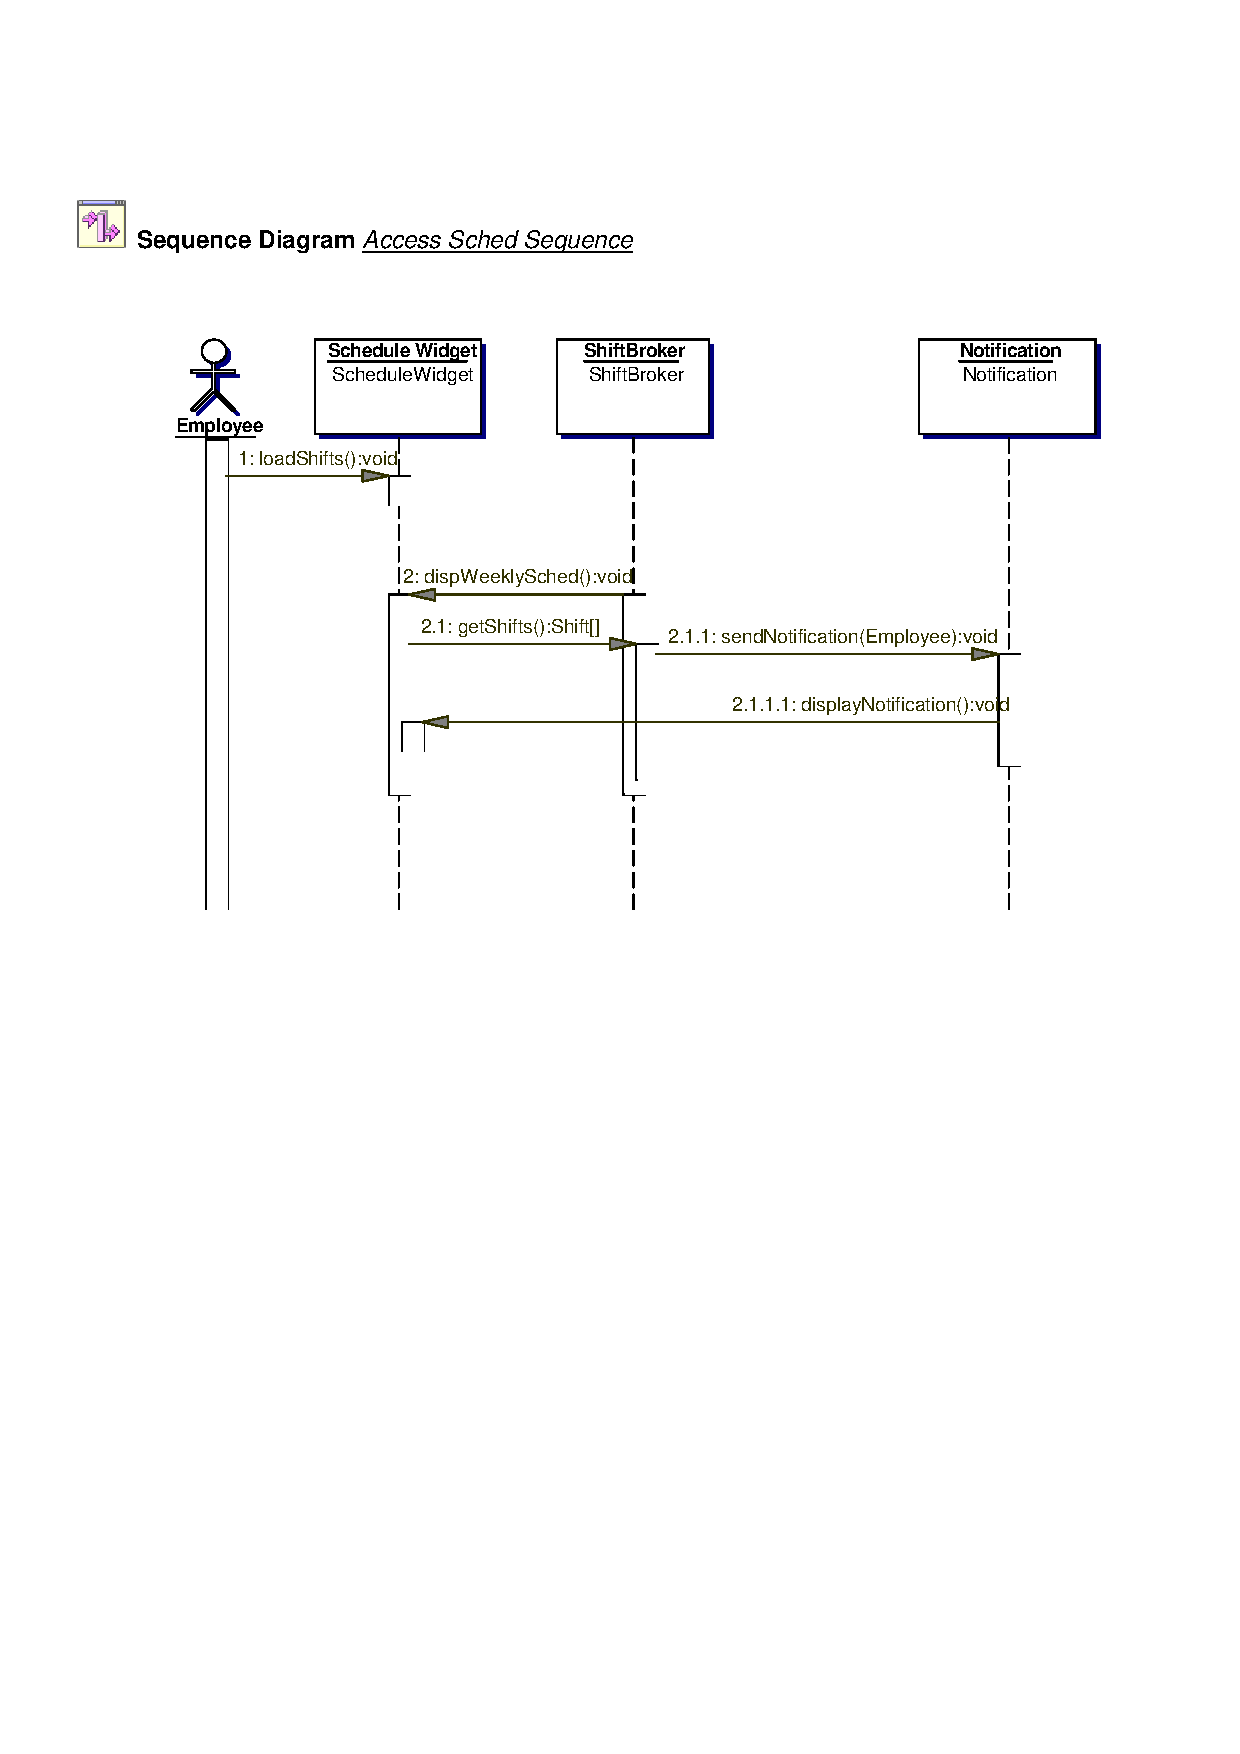
\includegraphics[scale=0.65]{externals/SequenceDiagrams1.pdf}
 \caption{\small
\textbf{Access Schedule Sequence Diagram}\newline A representation of the proper sequence for accessing an Employee`s Schedule}\label{fig:seqAccessSched}
\end{figure}
\newpage
\begin{figure}[hbp]
 \section{Add Supervisor Sequence Diagram}
 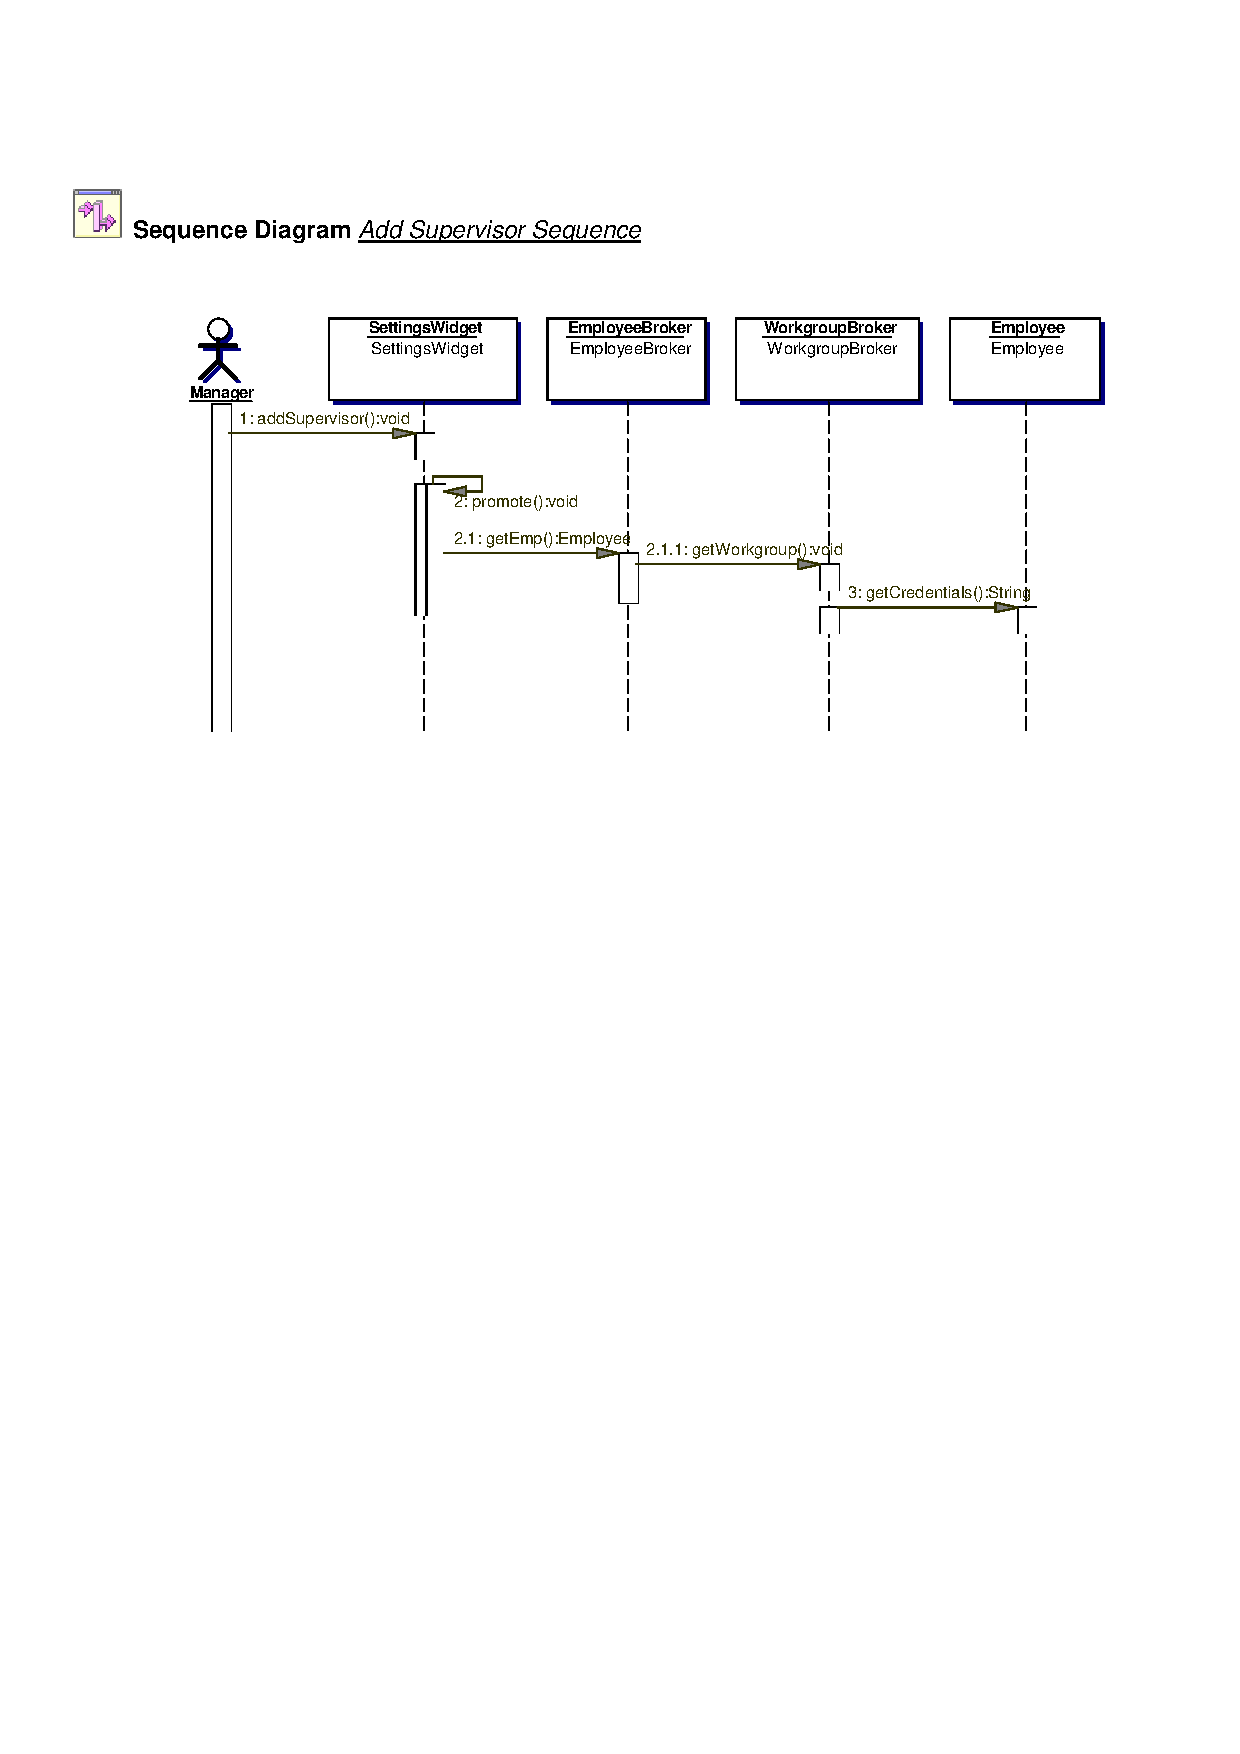
\includegraphics[scale=0.65]{externals/SequenceDiagrams2.pdf}
 \caption{\small
\textbf{Add Supervisor Sequence Diagram}\newline A representation of the proper sequence for creating an employee with supervisor permissions}\label{fig:seqAddSupervisor}
\end{figure}
\newpage
\begin{figure}[hbp]
 \section{Create Employee Type Sequence Diagram}
 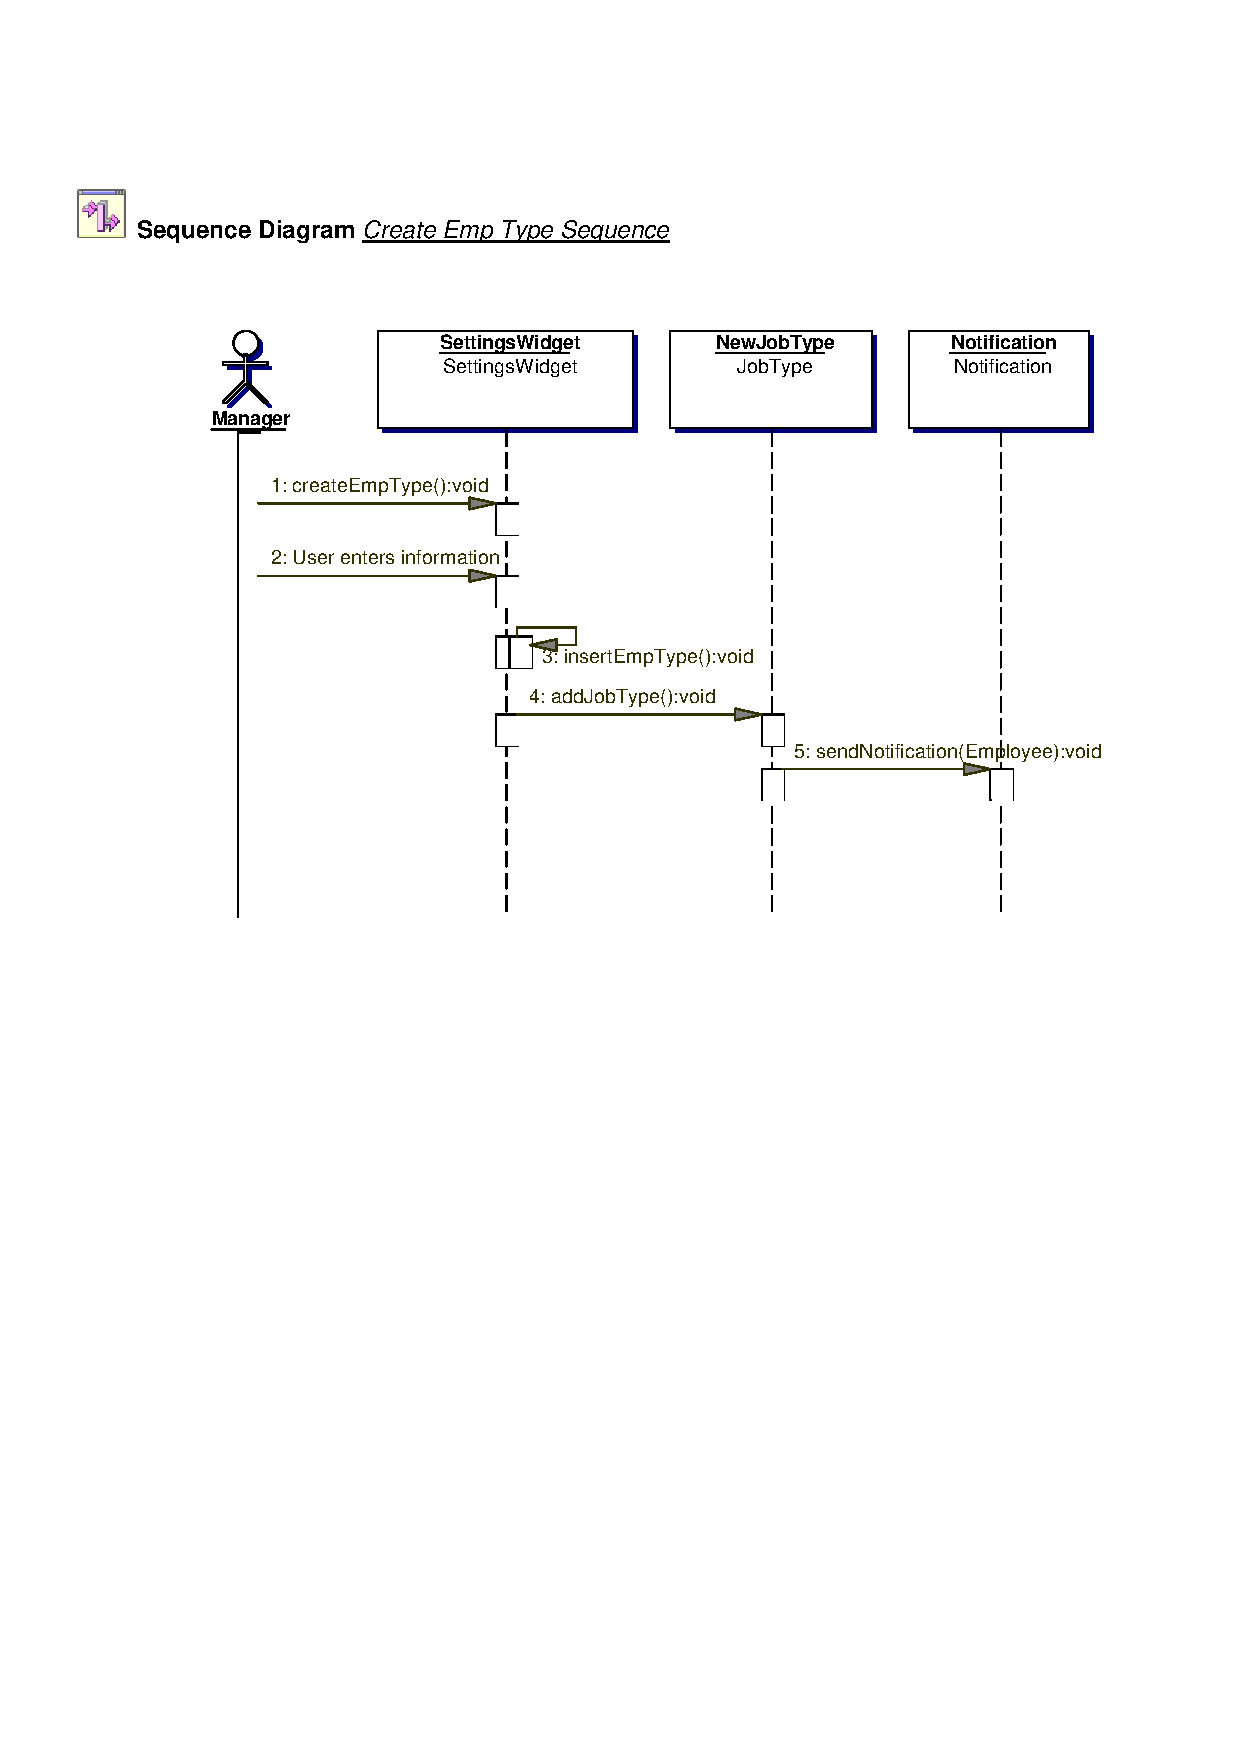
\includegraphics[scale=0.65]{externals/SequenceDiagrams3.pdf}
 \caption{\small
\textbf{Create Employee Type Sequence Diagram}\newline A representation of the proper sequence for creating an employee to work a specific job}\label{fig:seqEmployeeType}
\end{figure}
\newpage
\begin{figure}[hbp]
 \section{Create New Employee Sequence Diagram}
 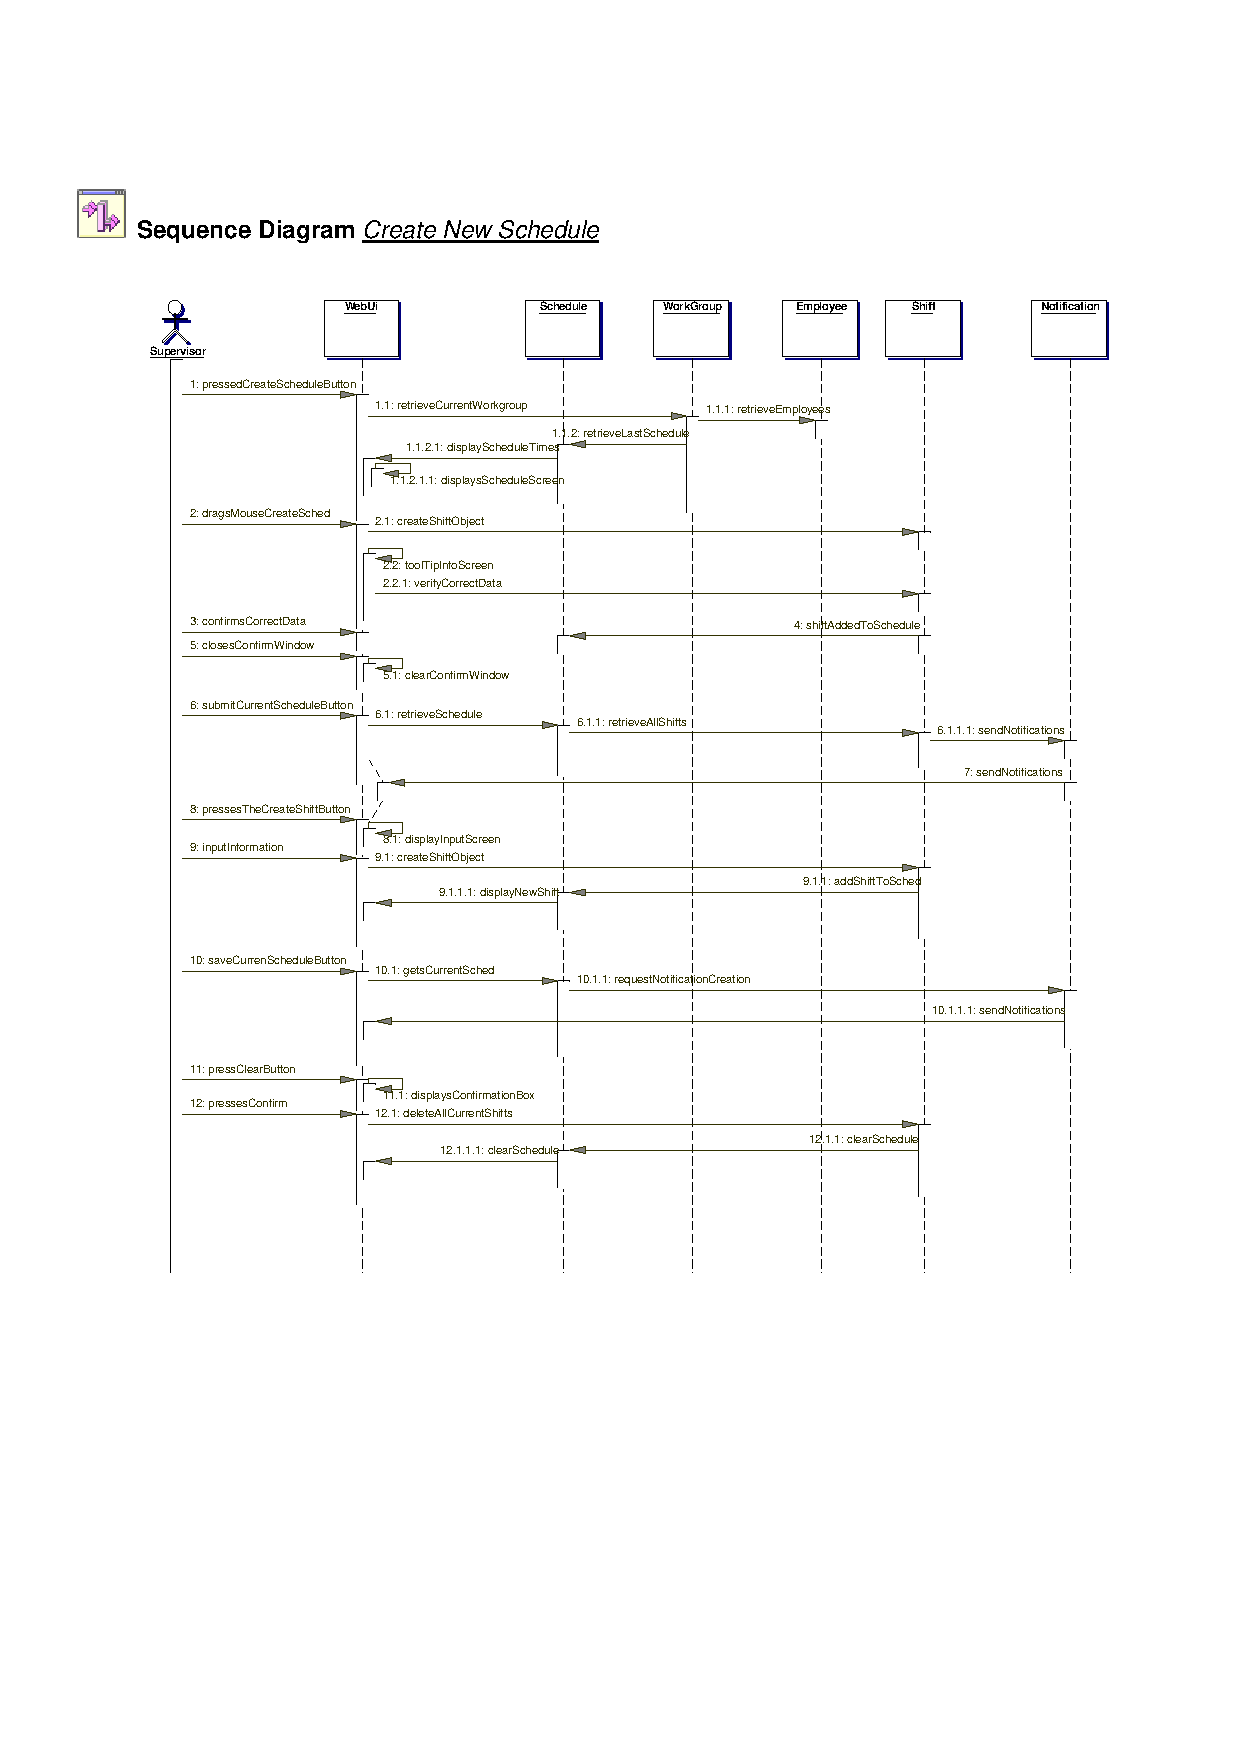
\includegraphics[scale=0.65]{externals/SequenceDiagrams4.pdf}
 \caption{\small
\textbf{Create New Employee Sequence Diagram}\newline A representation of the proper sequence for creating a new employee}\label{fig:seqCreateNewEmp}
\end{figure}
\newpage
\begin{figure}[hbp]
 \section{Distribute Report Schedule Sequence Diagram}
 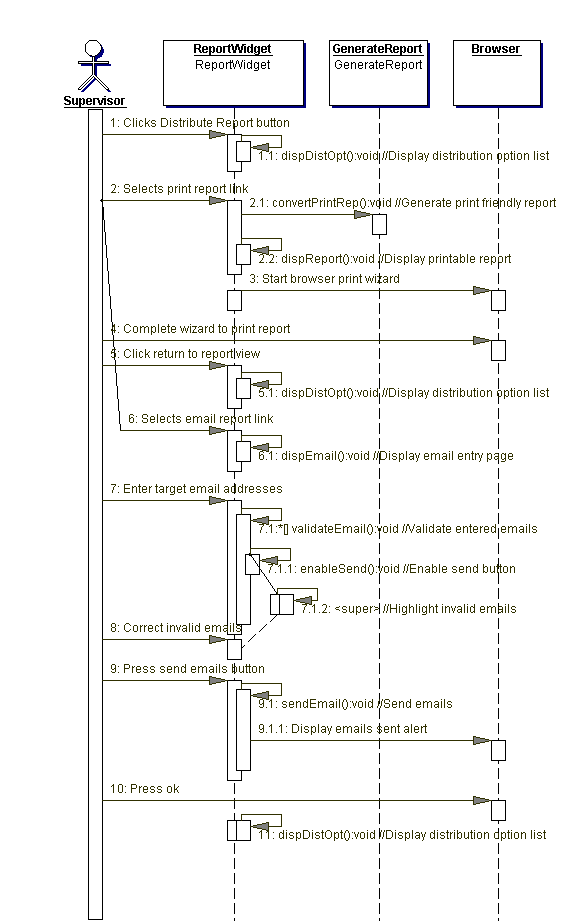
\includegraphics[scale=0.8]{externals/DistributeReportSequence.png}
 \caption{\small
\textbf{Distribute Report Sequence Diagram}\newline A representation of the proper sequence for distributing reports that are created}\label{fig:seqAccessSched}
\end{figure}
\newpage
\begin{figure}[hbp]
 \section{Generate Report Schedule Sequence Diagram}
 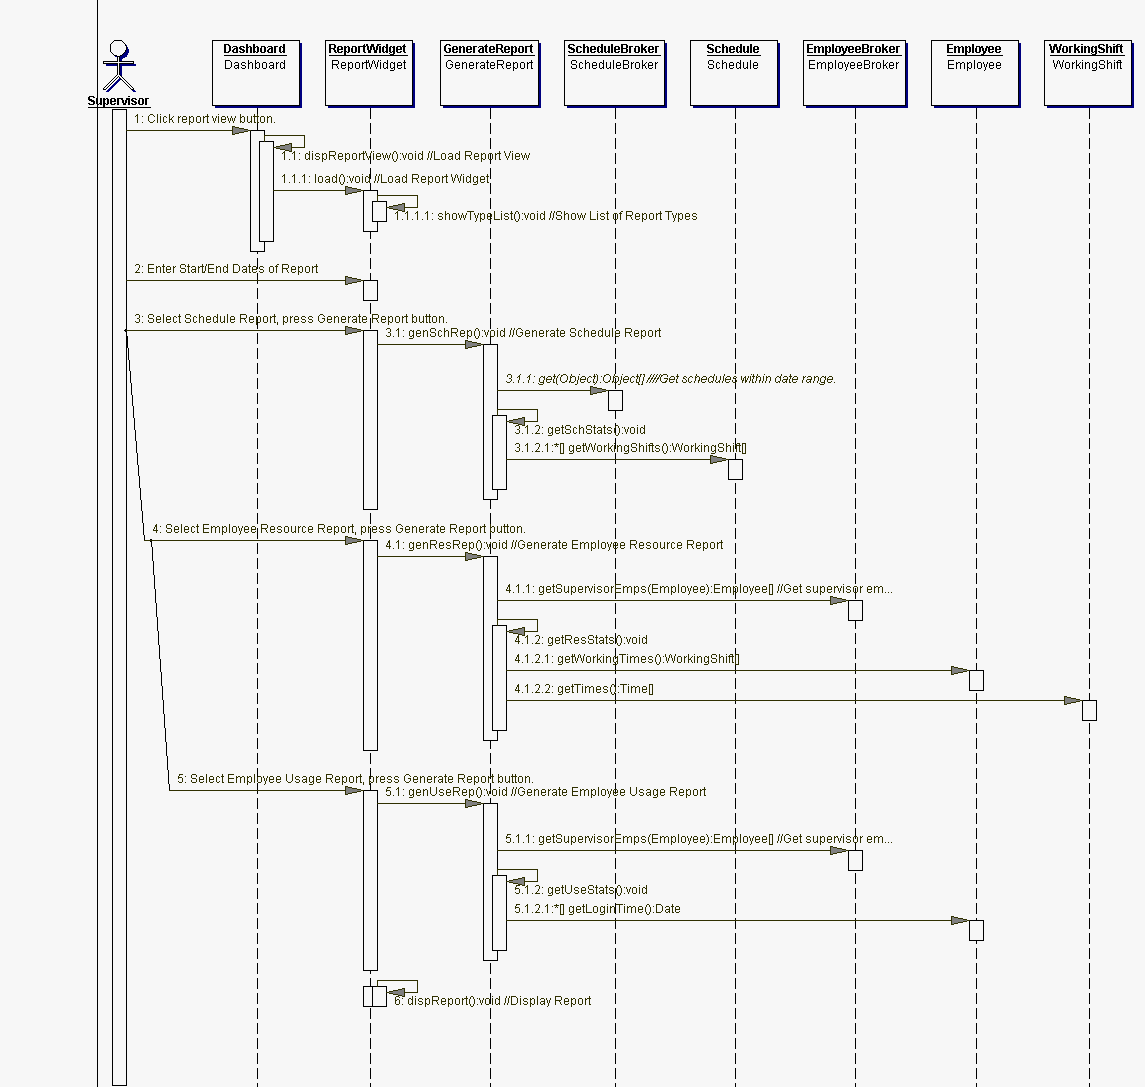
\includegraphics[scale=0.5]{externals/GenerateReportSequence.png}
 \caption{\small
\textbf{Generate Report Schedule Sequence Diagram}\newline A representation of the proper sequence for generating reports}\label{fig:seqGenReport}
\end{figure}
\newpage
\begin{figure}[hbp]
 \section{System Log In Sequence Diagram}
 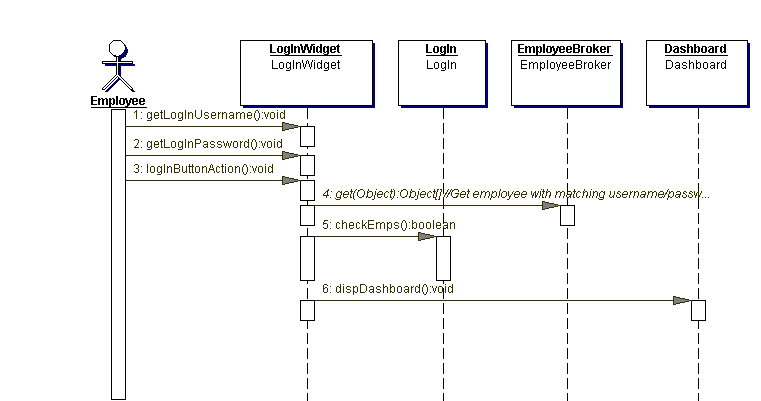
\includegraphics[scale=0.8]{externals/LogInSequence.png}
 \caption{\small
\textbf{System Log In Sequence Diagram}\newline A representation of the proper sequence for logging into the system}\label{fig:seqLogInSys}
\end{figure}
\newpage
\begin{figure}[hbp]
 \section{Maintain Workgroup Sequence Diagram}
 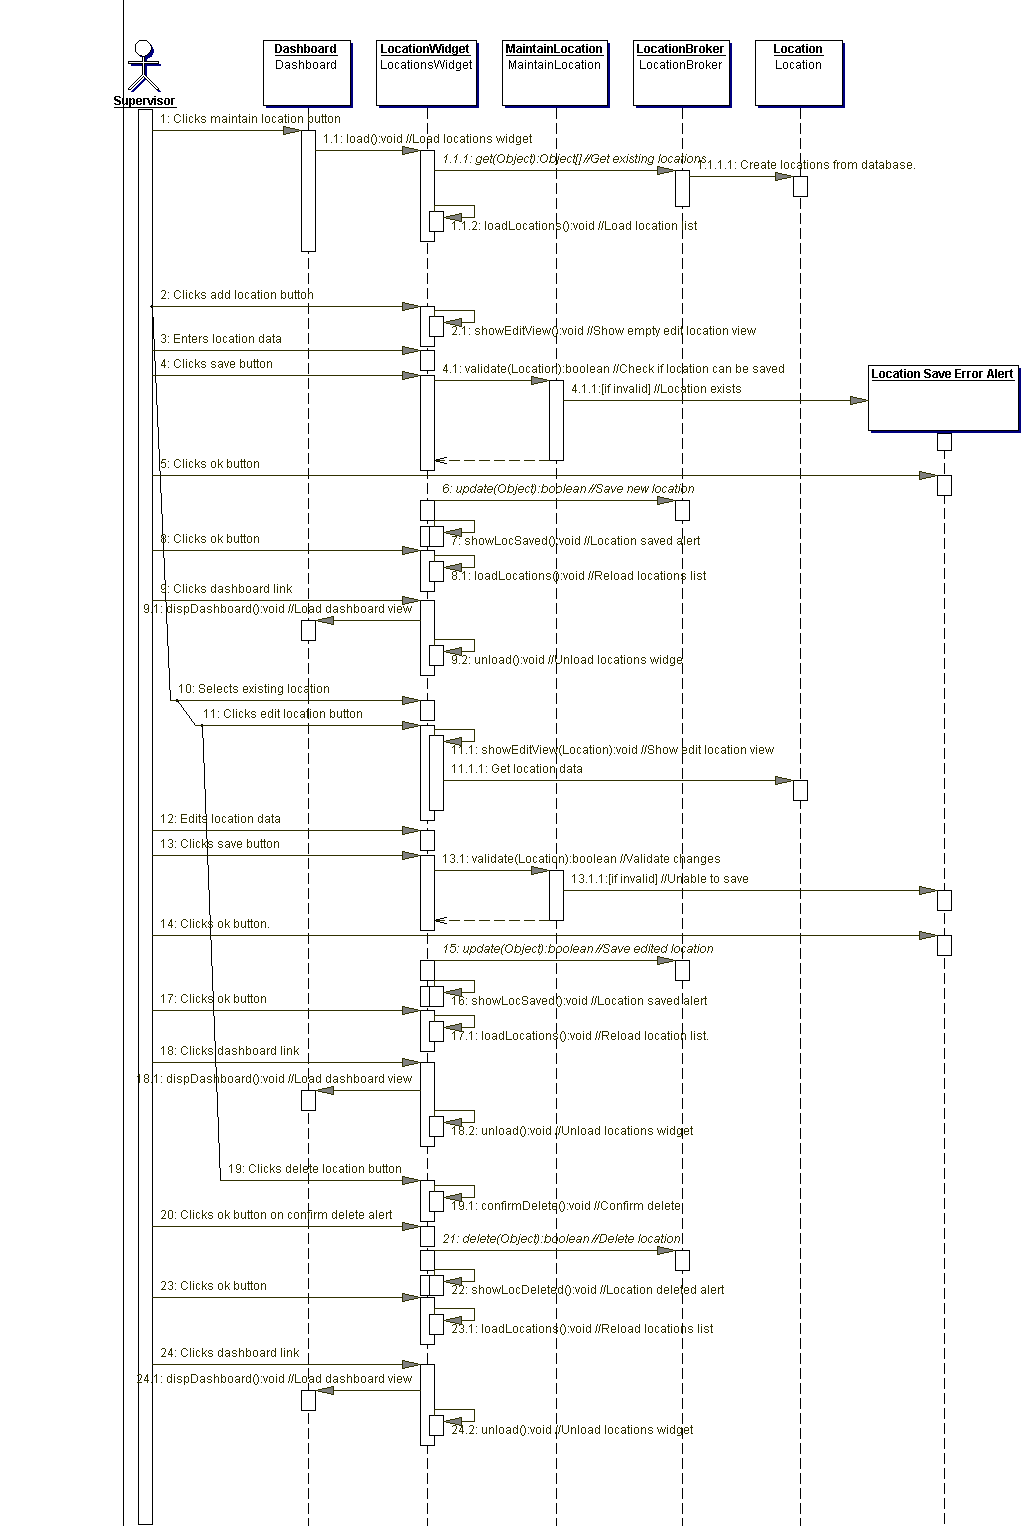
\includegraphics[scale=0.5]{externals/MaintainLocationSequence.png}
 \caption{\small
\textbf{Maintain Workgroup Sequence Diagram}\newline A representation of the proper sequence for editing workgroups to the desired situation}\label{fig:seqMaintainWkgrp}
\end{figure}
\newpage
\begin{figure}[hbp]
 \section{Maintain Position Sequence Diagram}
 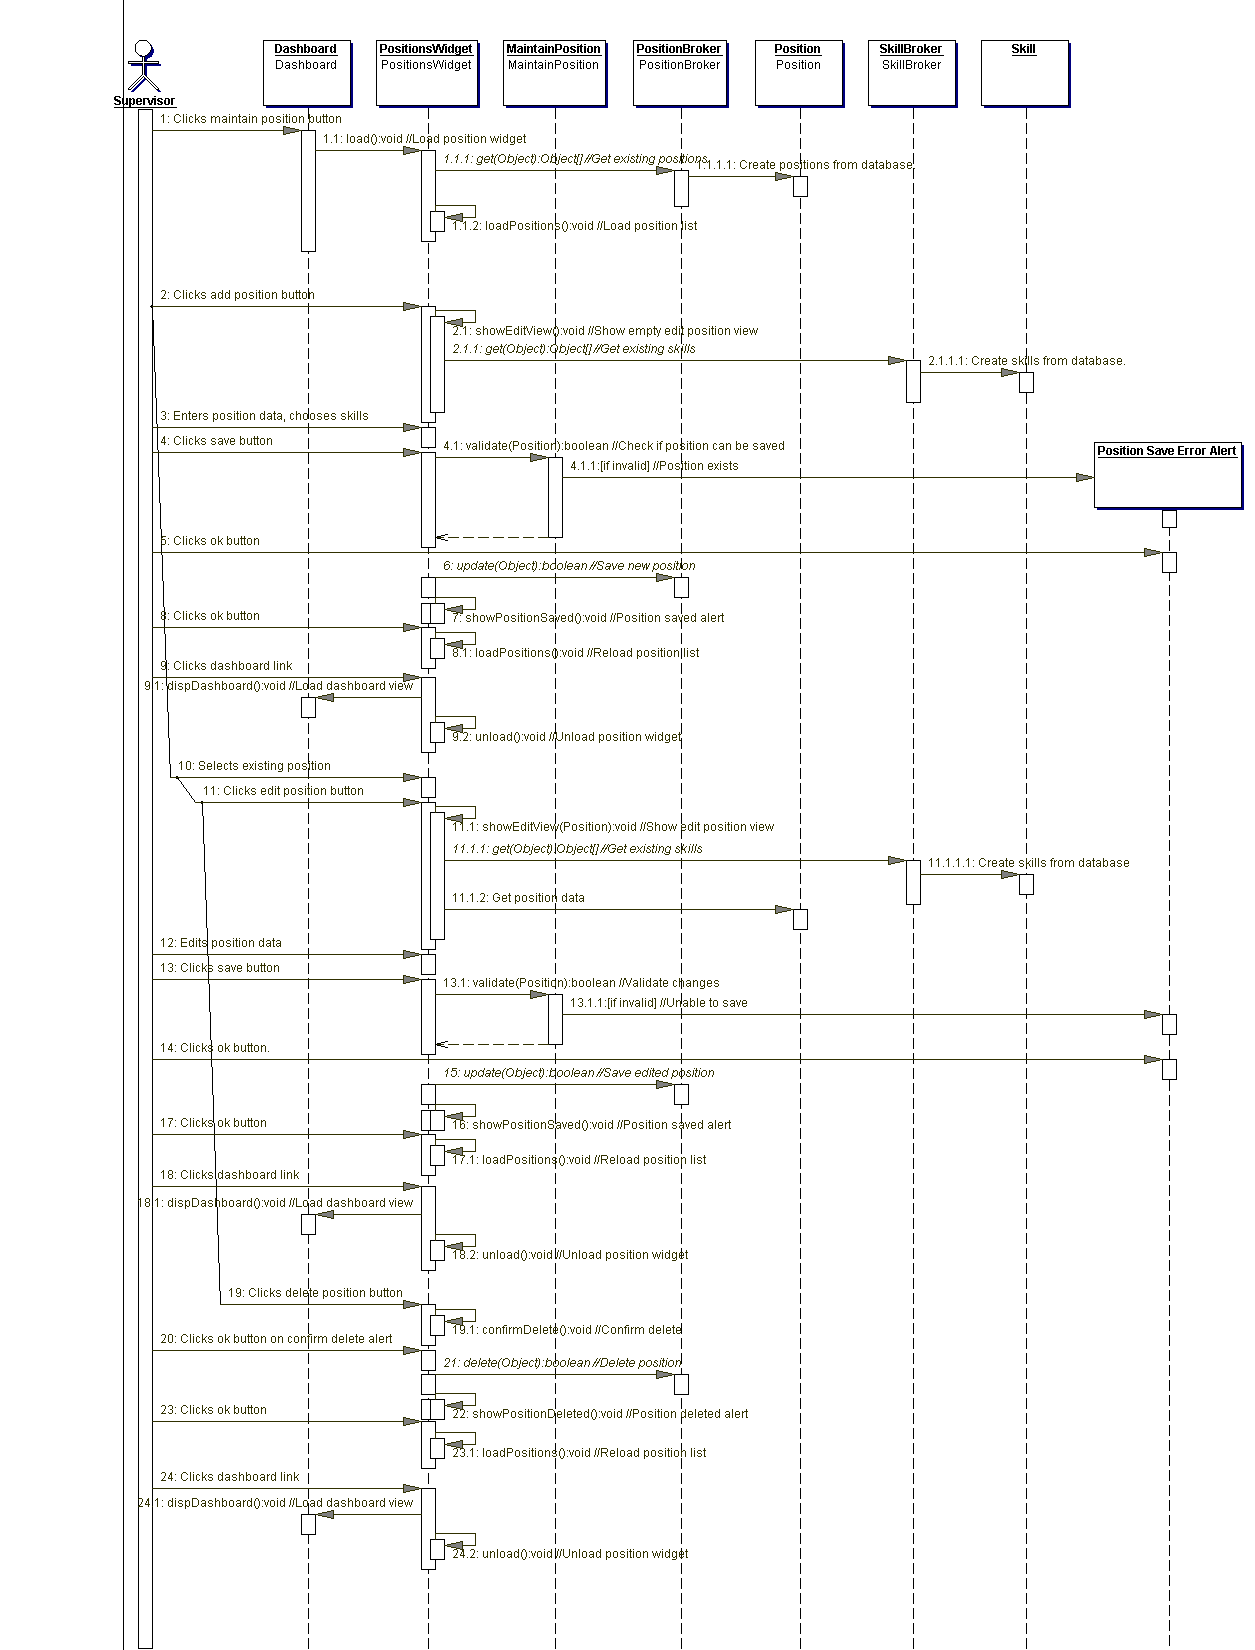
\includegraphics[scale=0.45]{externals/MaintainPositionSequence.png}
 \caption{\small
\textbf{Maintain Employee Sequence Diagram}\newline A representation of the proper sequence for editing an employee`s position to the desired situation}\label{fig:seqMaintEmp}
\end{figure}
\newpage
\begin{figure}[hbp]
 \section{Maintain Skill Sequence Diagram}
 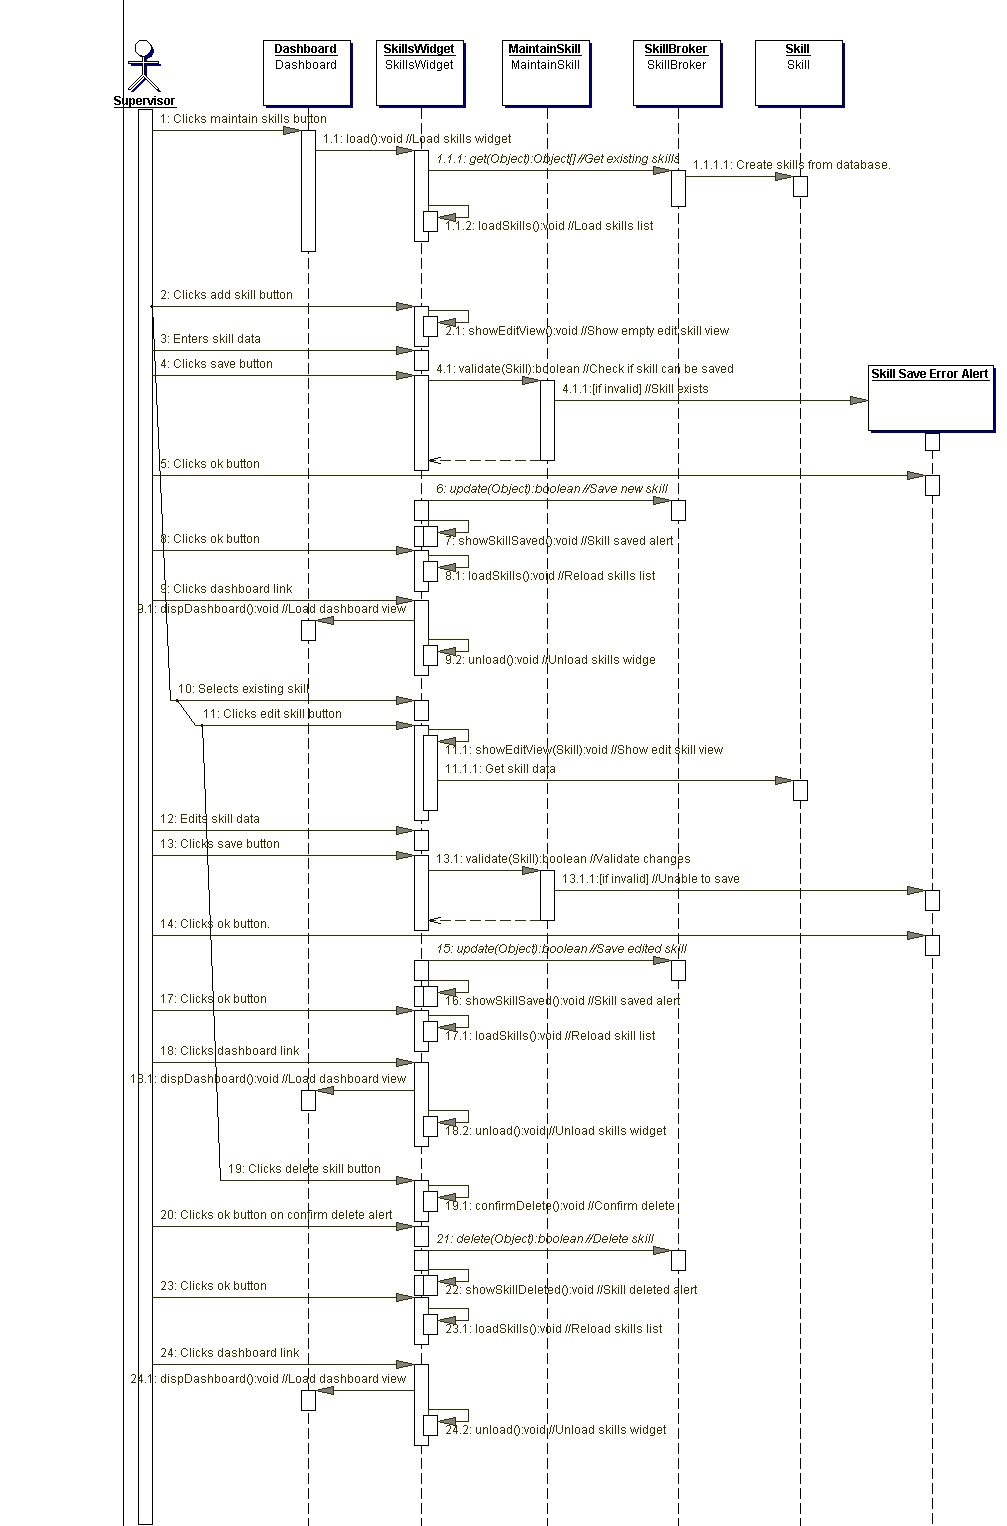
\includegraphics[scale=0.45]{externals/MaintainSkillSequence.png}
 \caption{\small
\textbf{Maintain Employee Sequence Diagram}\newline A representation of the proper sequence for editing an employee`s skills regarding the desired situation}\label{fig:seqMaintEmp}
\end{figure}
\newpage
\begin{figure}[hbp]
 \section{Review Request Sequence Diagram}
 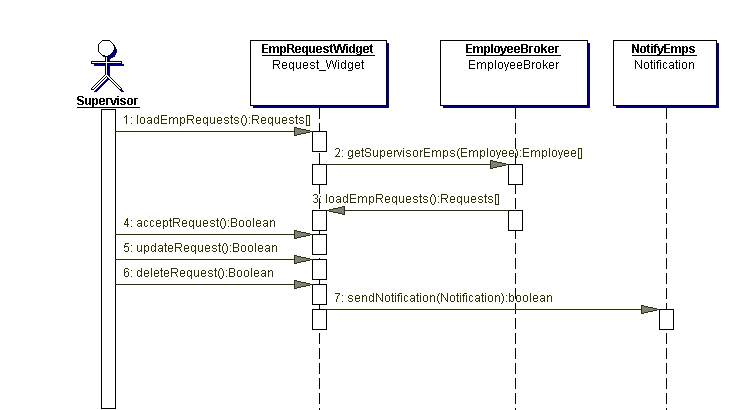
\includegraphics[scale=0.85]{externals/ReviewEmployeeRequestSequence.png}
 \caption{\small
\textbf{Review Request Sequence Diagram}\newline A representation of the proper sequence for reviewing an employee request by an authoritative employee}\label{fig:seqMaintEmp}
\end{figure}
\newpage
\begin{figure}[hbp]
 \section{Send Event Sequence Diagram}
 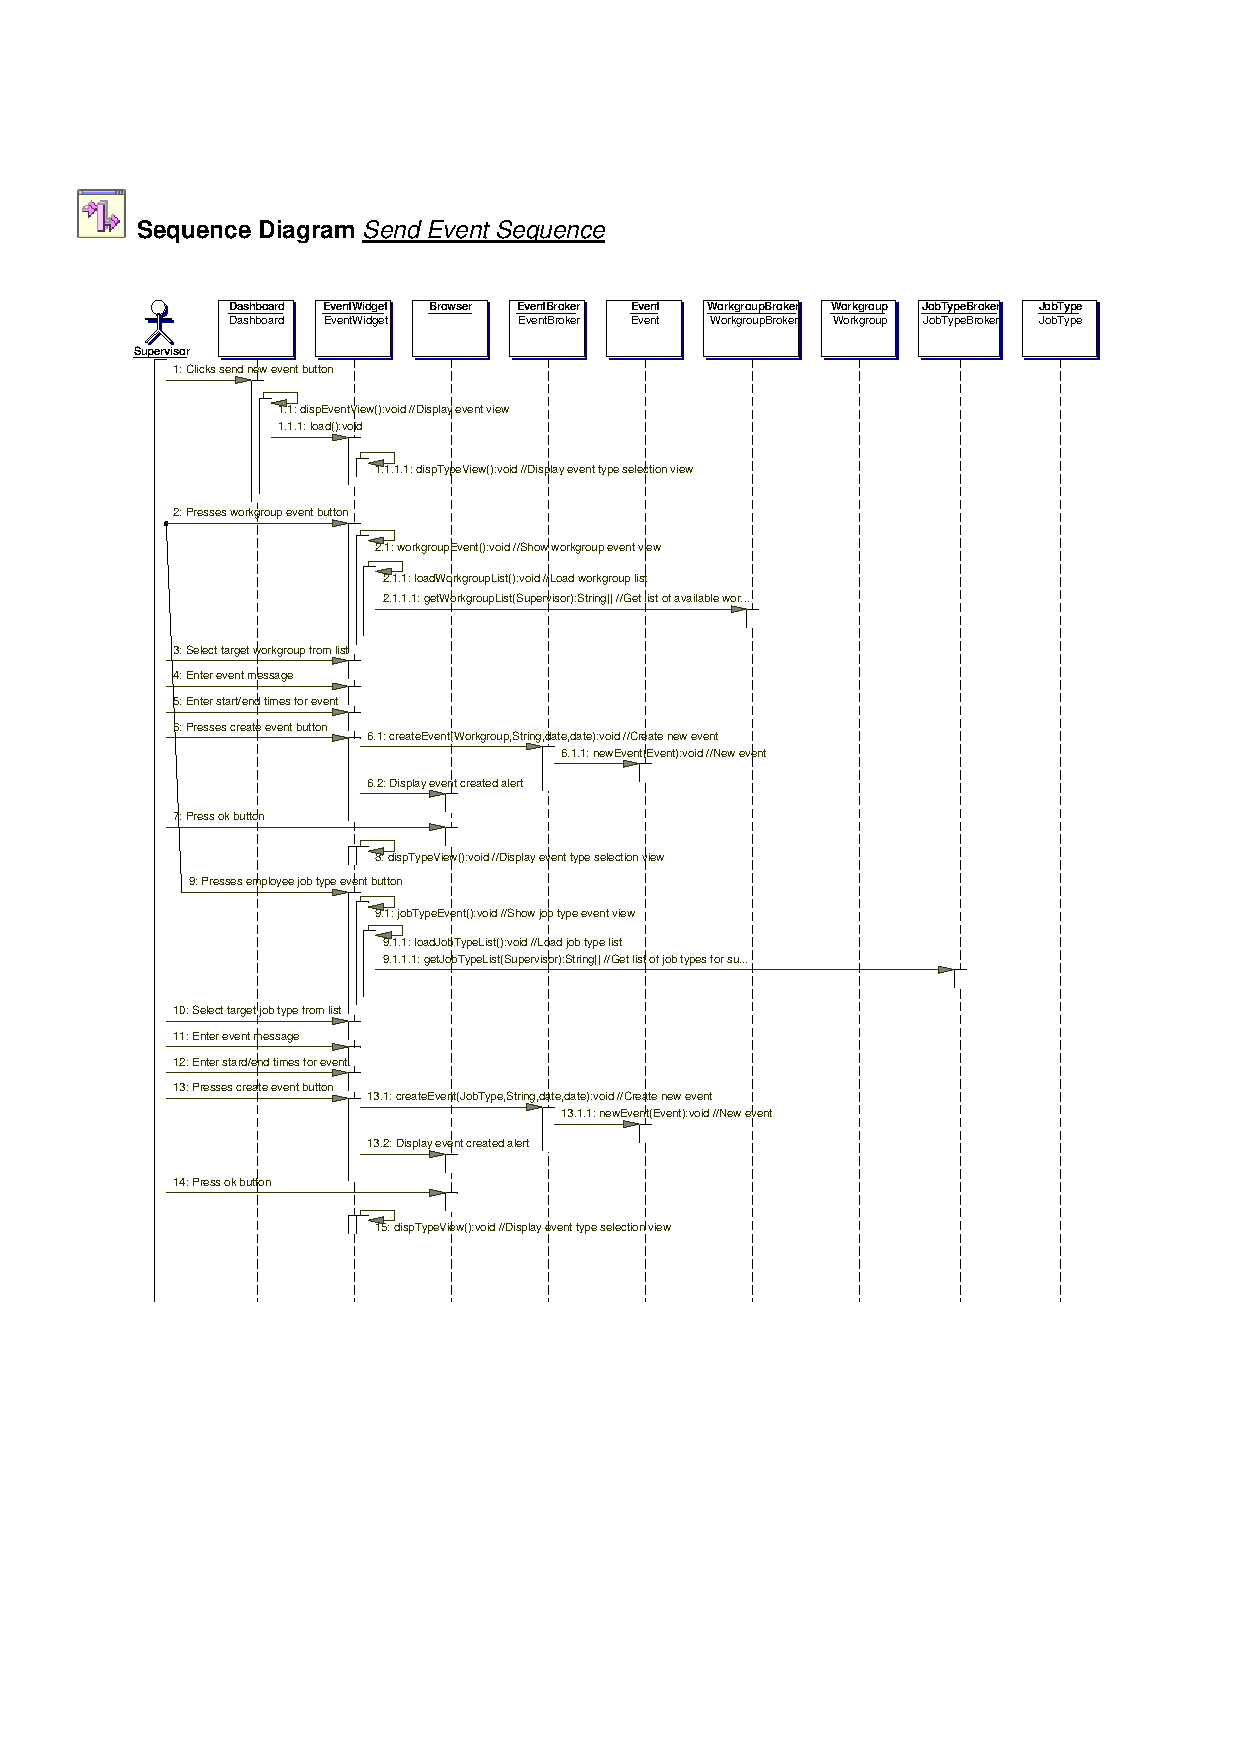
\includegraphics[scale=0.65]{externals/SequenceDiagrams11.pdf}
 \caption{\small
\textbf{Send Event Sequence Diagram}\newline A representation of the proper sequence for posting an event that certain groups of employees will see}\label{fig:seqSendEvent}
\end{figure}
\newpage
\begin{figure}[hbp]
 \section{Book Days Off Sequence Diagram}
 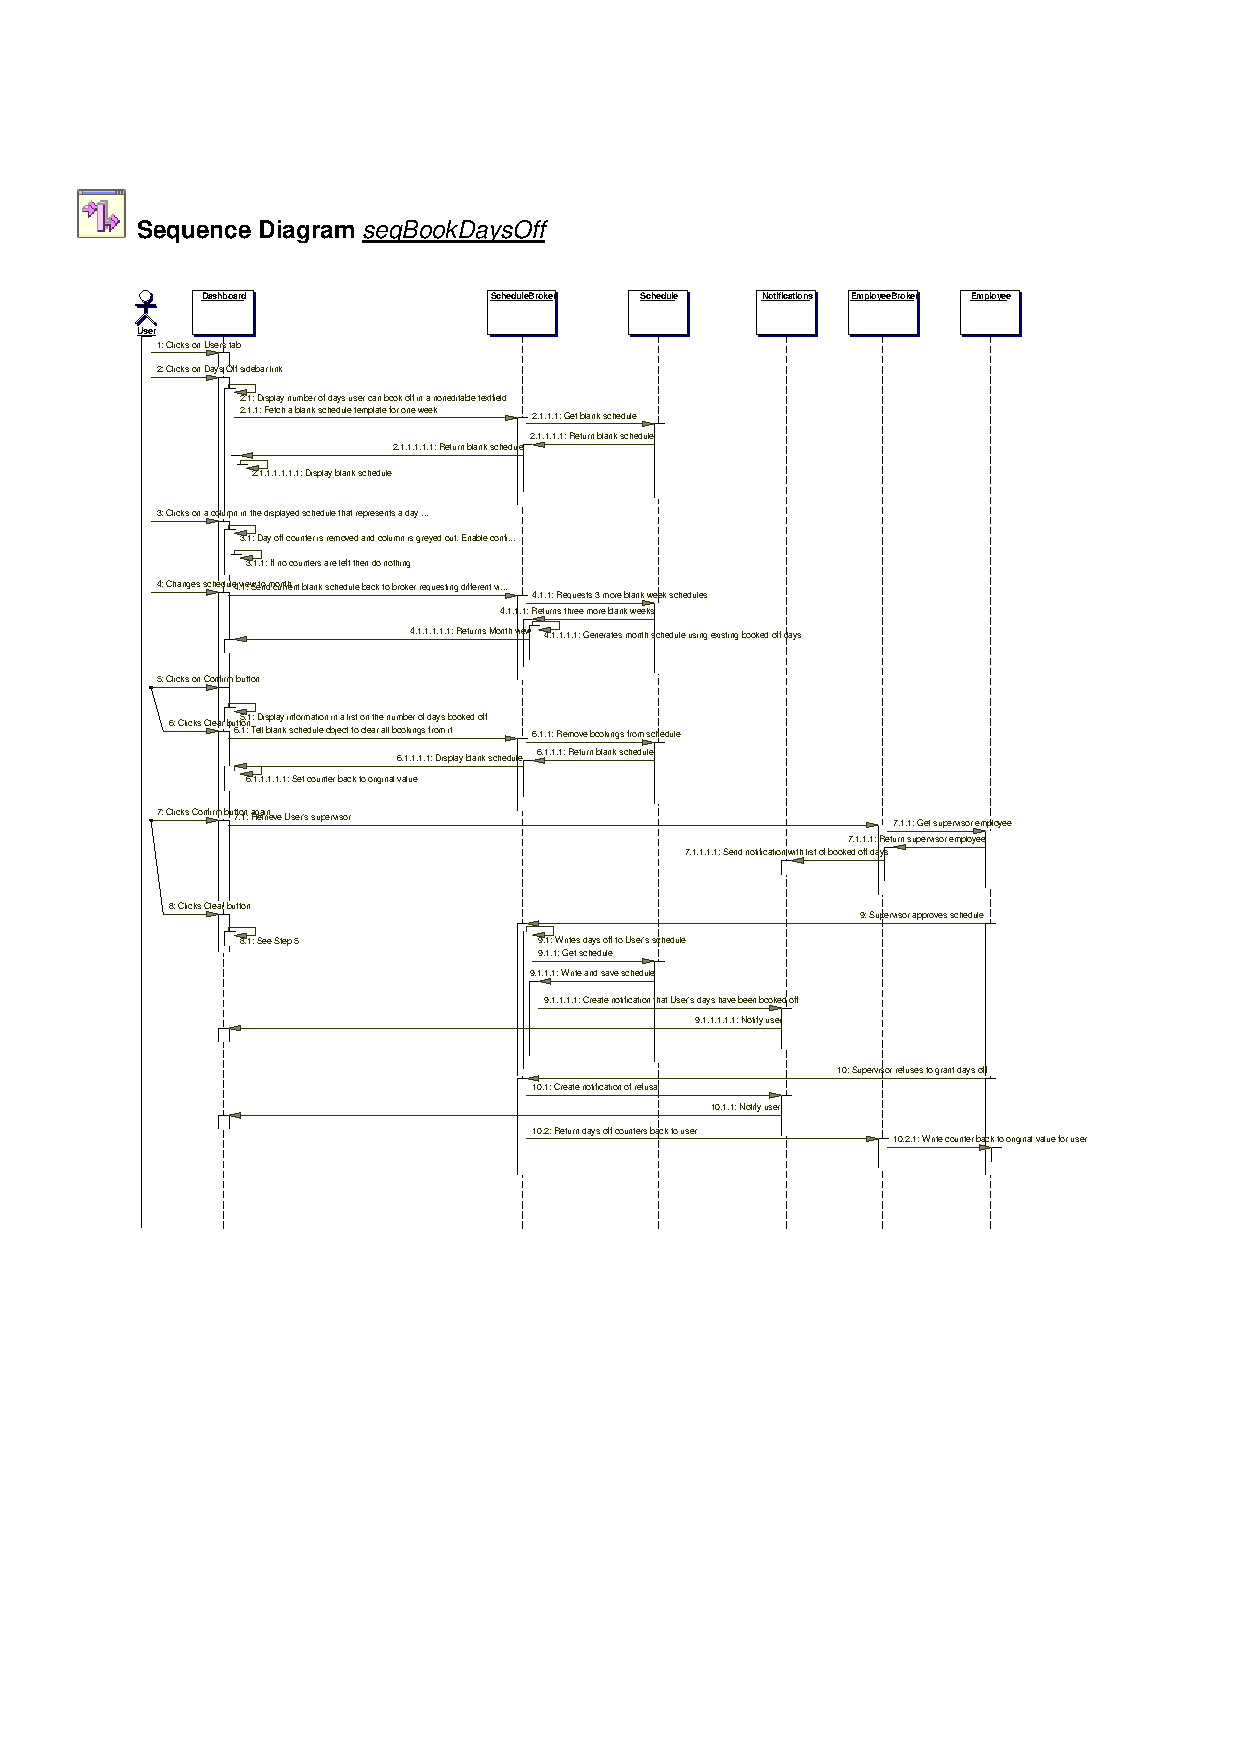
\includegraphics[scale=0.65]{externals/SequenceDiagrams12.pdf}
 \caption{\small
\textbf{Book Days Off Sequence Diagram}\newline A representation of the proper sequence for an employee to reduce working days in their schedule}\label{fig:seqBookDaysOff}
\end{figure}
\newpage
\begin{figure}[hbp]
 \section{Manager View Schedules Sequence Diagram}
 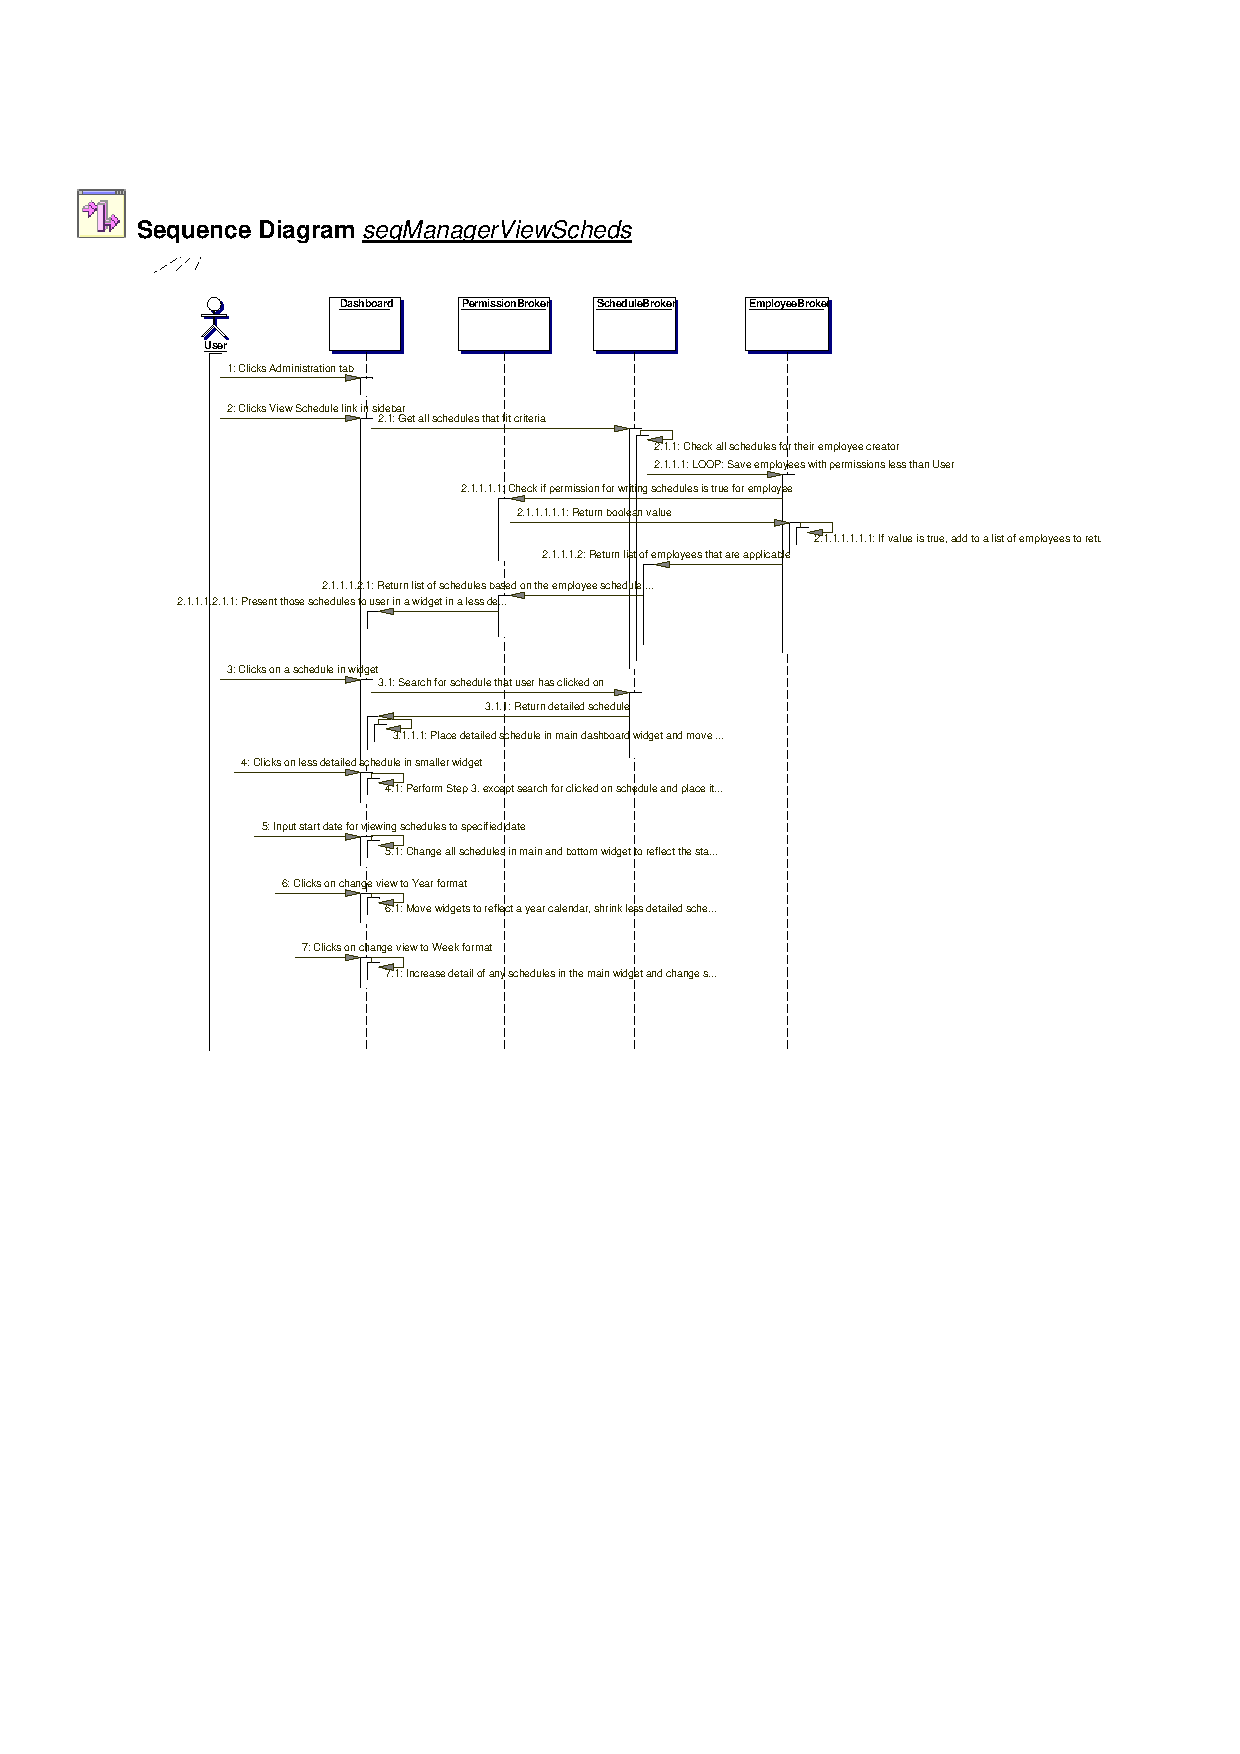
\includegraphics[scale=0.65]{externals/SequenceDiagrams13.pdf}
 \caption{\small
\textbf{Manager View Schedules Sequence Diagram}\newline A representation of the proper sequence for a Manager to view multiple schedules at one time}\label{fig:seqManagerView}
\end{figure}
\newpage
\clearpage

\begin{figure}[hbp]
 \section{Request Shift Change Sequence Diagram}
 \includegraphics[scale=0.65]{externals/SequenceDiagrams14.pdf}
 \caption{\small
\textbf{Request Shift Change Sequence Diagram}\newline A representation of the proper sequence for requesting another user to take or exchange shifts with}\label{fig:seqShiftChange}
\end{figure}
\newpage
\begin{figure}[hbp]
 \section{Update Availability Sequence Diagram}
 \includegraphics[scale=0.65]{externals/SequenceDiagrams15.pdf}
 \caption{\small
\textbf{Update Availability Sequence Diagram}\newline A representation of the proper sequence for changing an employee`s available work times}\label{fig:seqUpdateAvail}
\end{figure}
\newpage
\begin{figure}[hbp]
 \section{Send Emergency Notification Sequence Diagram}
 \includegraphics[scale=0.65]{externals/SequenceDiagrams18.pdf}
 \caption{\small
\textbf{Send Emergency Notification Sequence Diagram}\newline A representation of the proper sequence for handling emergencies that prevent employee`s presence at work}\label{fig:seqEmergency}
\end{figure}
\newpage
\begin{figure}[hbp]
 \section{View Workgroup Schedule Sequence Diagram}
 \includegraphics[scale=0.65]{externals/SequenceDiagrams17.pdf}
 \caption{\small
\textbf{View Workgroup Schedule Sequence Diagram}\newline A representation of the proper sequence for viewing schedules of employees working for one job type}\label{fig:seqViewWorkgroup}
\end{figure}
\newpage

\chapter{Data Dictionary}\index{Data Dictionary}
\newpage
\section{Interface}
\includegraphics[scale=0.9,trim=10mm 30mm 25mm 35mm]{externals/di1.pdf}
\newpage
\includegraphics[scale=0.9,trim=20mm 30mm 25mm 25mm]{externals/di2.pdf}
\newpage
\includegraphics[scale=0.9,trim=20mm 30mm 25mm 25mm]{externals/di3.pdf}
\newpage
\includegraphics[scale=0.9,trim=20mm 30mm 25mm 25mm]{externals/di4.pdf}
\newpage
\includegraphics[scale=0.9,trim=20mm 30mm 25mm 25mm]{externals/di5.pdf}
\newpage
\includegraphics[scale=0.9,trim=20mm 30mm 25mm 25mm]{externals/di6.pdf}
\newpage
\includegraphics[scale=0.9,trim=20mm 30mm 25mm 25mm]{externals/di7.pdf}
\newpage
\includegraphics[scale=0.9,trim=20mm 30mm 25mm 25mm]{externals/di8.pdf}
\newpage
\includegraphics[scale=0.9,trim=20mm 30mm 25mm 25mm]{externals/di9.pdf}
\newpage
\includegraphics[scale=0.9,trim=20mm 30mm 25mm 25mm]{externals/di10.pdf}
\newpage
\includegraphics[scale=0.9,trim=20mm 30mm 25mm 25mm]{externals/di11.pdf}
\newpage
\includegraphics[scale=0.9,trim=20mm 30mm 25mm 25mm]{externals/di12.pdf}
\newpage
\section{Persistence}
\includegraphics[scale=0.9,trim=10mm 30mm 25mm 35mm]{externals/dp1.pdf}
\newpage
\includegraphics[scale=0.9,trim=20mm 30mm 25mm 25mm]{externals/dp2.pdf}
\newpage
\includegraphics[scale=0.9,trim=20mm 30mm 25mm 25mm]{externals/dp3.pdf}
\newpage

\section{Application Domain}

\includegraphics[scale=0.9,trim=20mm 30mm 25mm 25mm]{externals/dd1.pdf}
\newpage
\includegraphics[scale=0.9,trim=20mm 30mm 25mm 0mm]{externals/dd2.pdf}
\newpage
\includegraphics[scale=0.9,trim=20mm 40mm 25mm 9mm]{externals/dd3.pdf}
\newpage
\includegraphics[scale=0.9,trim=20mm 30mm 25mm 0mm]{externals/dd4.pdf}
\newpage
\includegraphics[scale=0.9,trim=20mm 30mm 25mm 0mm]{externals/dd5.pdf}
\newpage

\section{Business Domain}
\includegraphics[scale=0.9,trim=10mm 30mm 25mm 10mm]{externals/db1.pdf}
\newpage
\includegraphics[scale=0.9,trim=20mm 30mm 25mm 8mm]{externals/db2.pdf}
\newpage
\includegraphics[scale=0.9,trim=20mm 30mm 25mm 0mm]{externals/db3.pdf}
\newpage
\includegraphics[scale=0.9,trim=20mm 30mm 25mm 0mm]{externals/db4.pdf}
\newpage
\includegraphics[scale=0.9,trim=20mm 30mm 25mm 8mm]{externals/db5.pdf}
\newpage
\includegraphics[scale=0.9,trim=20mm 30mm 25mm 8mm]{externals/db6.pdf}
\newpage
\includegraphics[scale=0.9,trim=20mm 30mm 25mm 8mm]{externals/db7.pdf}
\newpage
\includegraphics[scale=0.9,trim=20mm 30mm 25mm 0mm]{externals/db8.pdf}
\newpage
\includegraphics[scale=0.9,trim=20mm 30mm 25mm 0mm]{externals/db9.pdf}
\newpage
\includegraphics[scale=0.9,trim=20mm 30mm 25mm 8mm]{externals/db10.pdf}
\newpage
\includegraphics[scale=0.9,trim=20mm 30mm 25mm 8mm]{externals/db11.pdf}
\newpage
\includegraphics[scale=0.9,trim=20mm 30mm 25mm 8mm]{externals/db12.pdf}
\newpage

\part{Project Management}\index{Project Management}

\chapter{Schedule}\index{Schedule}
\section{Gantt Chart}

\begin{figure}[htp]
  \includegraphics[scale=0.9, trim=10mm 10mm 10mm 15mm]{externals/webagenda_gantt.pdf}
\label{fig:gantt1}
\end{figure}

\pagebreak

\section{2009 -10-08 – Requirements Documentation}\index{Requirements Documentation}
\hspace{1cm}The requirements documentation is a compilation of details on the WebAgenda\index{WebAgenda} \index{WebAgenda}project\index{project}. This document is used to outline the specific user requirements of the project, the \textbf{system requirements}\index{System Requirements} of the project, the \textbf{system interface requirements}\index{system interface} of the project, and the project management details of the project.
\paragraph*{}Inside the user requirements portion of the document, the business overview and objectives need to be defined. This includes the nature of the client’s business, the mission of the business and all other relative information in regards to the client’s business model. A project\index{project} overview should also be included in the documentation. It should include things like a statement of the current problem or issue the client has with their current system\index{system}. The \textbf{project scope}\index{project scope} should also be included with the project overview. This should include things like what the system\index{system} needs to be able to do and include a summary of the major functional requirements\index{Functional Requirements} of the system. The system environment will also be included in the project overview. The scope of the project details what the system will be able to do and what it will not be able to do. In other words, the scope just outlines the project boundaries. The system environment is also included in the project overview and details where the project will be deployed upon \textbf{beta release}\index{Beta Release} and \textbf{final releases}. The project overview will include a description of the current system and what the type of functionality it has in addition to its downfalls and the desired improvements.
% ReWord this when time is available
\paragraph*{}The next section of the requirements document is the project\index{project} system\index{system} requirements. The first point of the system requirements\index{System Requirements} is the fact-finding methodology\index{Fact-Finding Methodology}. This will include a description of the approach project team members took to find facts regarding the system. Any questions that were asked in the interview process will also be included in the fact-finding methodology section of the system requirements\index{System Requirements}. A use case\index{Use Case} diagram that was derived from the fact-finding process should also be included in the system requirements section. A description of the use case\index{Use Case} elements should also be included in this section, things like \index{actor}actor definition, and roles should be defined in this section. A non-functional requirement should also be derived here from the use case and the fact-finding section of the system requirements. A system interface\index{System Interface Requirements} requirements section should also be included and derived from the use case and fact-finding sections. \textbf{Maintainability}\index{Maintainability} and Administration requirements\index{Administration Requirements} should also be included in this section. This means things like maintenance and backup\index{Backup} schedules, and all administration aspects that the system needs to include to have the full functionality that the current system has. Usability requirements should also be included in this section. The usability requirements includes things like how advanced the users are at using software/computers in general. This should also include how many people will be using the software and how familiar they are with software/computers in general.
\pagebreak

\section{2009-11-05 – Requirements Analysis}\index{Requirements Analysis}
\hspace{1cm}The requirements analysis is incorporated into the project\index{project} planning stages of the project by identifying how close the requirements are to the actual project features. Once the project team meets with the client and determines exactly what the client wants, the updated features list then is located in the requirements analysis. Changes to the original requirements documentation will go into the requirements Analysis report. The client should receive both a copy of the requirements documentation and the requirements analysis to ensure that it is up to date and accurate. 
\section{2009-12-17 – Design Documentation}\index{Design Documentation}
\hspace{1cm}The design documentation is the final piece of documentation in the planning stages of the project\index{project}. It is an all inclusive summary of all the client’s technical and informational requirements for the project. This includes budget, time constraints, and any final technical specifications for the project. The design documentation should be used by the developers as a reference when building the project. If any questions arise as to features of the project the developers should consult the design documentation for conclusion. It is the most up to date compilation from the client and the developers about the project.\newline
\paragraph*{}\hspace{1cm} Included in the design document is design related functionality. How the system\index{system} needs to be implemented needs to be considered at this stage. Information regarding the human computer interface\index{interface} needs to be seriously considered here. All interface related documentation needs to be reflected in both the sequence diagrams and the problem domain class diagram.\newline
\paragraph*{}\hspace{1cm} Hardware architecture needs to be described in this document. Minimum hardware specifications for properly running the software need to be outlined in this document. Software architecture also needs to be implemented. Minimum software requirements need to be outlined in this document as well. Any software dependencies need to be outlined and documented in this document so the user can see what software they need in order to run the system\index{system}.
\pagebreak
\section{2009-01-30 – Alpha Release}\index{Alpha Release}
\hspace{1cm}The pre-beta release\index{Beta Release}, known as an \textbf{alpha release}, is a basic functional release of the software. The software may have next to no features of the full release and the ones that do exist are partially tested and potentially have \textbf{bug}s\index{bug}. The alpha release is used to start working out bugs and get any input from the client as to features that need to be modified or changed to meet the client’s needs. The interface\index{interface} may need some changes at this stage to incorporate other features.
\section{2009-02-28 – Beta Release}\index{Beta Release}
\hspace{1cm}The beta release will have full functionality of the final software, with the exception of plug-ins. However, there will probably be bugs\index{bug} in the program. This release of the software is meant to work out any bugs and ensure that the software is acceptably tested. The software at this stage will also get stress tested, meaning that testers and possibly the client need to use the program and purposely try to break it. This way we can find bugs that may not have surfaced at the alpha stage and fix them before the final release\index{Final Release}. This stage should include any minor adjustments that the client requests. 
\section{2009-04-15 – Final Release}\index{Final Release}
\hspace{1cm}The final release will be a full featured, and fully tested release. The software will have all the features that the client requested as well as all the other features that the system\index{system} implements within the scope of the project\index{project}. Having tested the software at both the alpha release\index{Alpha Release} and the beta release\index{Beta Release}, most of the major bugs\index{bug} should be worked out by the final release period. Some minor bugs may still be in the system but they should not influence productivity or stability at all. The software needs to be in a safe usable state. All \textbf{encryption}\index{encryption} and \textbf{SSL}\index{SSL} features need to be implemented so that the users can fully use the software without worrying about any security flaws. The software should also be deployment\index{Deployment} ready, so that it can be installed and go live on the users system. 

\chapter{Team Configuration}\index{Team Configuration}
	The following section provides detail on the team members involved in the project\index{project}, as well as their current roles. Contact information is included for team members as well as other key stakeholders.

\section{Members And Roles}\index{Members And Roles}
The following people are the members of the project\index{project} team.  Current role assignments are included and described.\newline
\newline
Mark Hazlett
\begin{itemize}
\item Team Leader – Ensures all team members understand their roles and what work is required from them each week.
\item Meeting Organizer – Schedules future meetings and ensures all team members are aware and able to attend.
\end{itemize}
Daniel Kettle
\begin{itemize}
\item Standards Checker – Ensures all documentation meets the guidelines listed in the Documentation Standards section of the Preface.
\item Archivist – Handles storage of documentation and other project\index{project} related files, ensuring they are freely accessible to the team.
\end{itemize}
\pagebreak
Daniel Wehr
\begin{itemize}
 \item Scribe – Distributes audio recordings of all meetings to group members on the same day they were recorded.  Meeting minutes will be typed up and submitted to the team for review before they are finalized and included in the project\index{project} documentation.
 \item Quality Assurance – Ensures non-documentation project\index{project} files such as source code\index{source code} meet the standards of the team and have been reviewed for efficiency.
\end{itemize}

\section{Reporting Relationships and Procedures}\index{Reporting Relationships and Procedures}
\hspace{1cm}All group members will be responsible for reporting the status of the project\index{project} to the client. The reporting position will be filled by individual members, and be rotated through on a regular basis as per agreement with the client. Current reporting periods are once a month, and since they will be in person the reports can be printed and sent electronically. Reports will be written, and will be sent to the client by email or fax.  The client will be given time to review the report, after which they will be contacted for their input on the progress that has been made to ensure the project is following their requirements.  All reports will be included in the project documentation for later reference.
\pagebreak
\section{Contact Information}\index{Contact Information}

\includegraphics{externals/contact.pdf}
\pagebreak

\chapter{Project Standards And Procedures}\index{Project Standards and Procedures}

\paragraph{}\hspace{0.6cm}\textbf{LaTeX2E} \index{LaTeX2E}, also known as \index{LaTeX}LaTeX, is a document preparation system\index{system} for high-quality typesetting. It has been used in various academic institutions and produces standardized and consistant pages based on tags specified in the LaTeX files. It is not a word processor; appearance is generated from the source file the user creates. Final documents will be generated as a pdf file.
LaTeX is also free and available for Windows, Mac, and Linux-Unix systems. The current version is 2E; it will be used for generating all digital-based final documentation. Since WebAgenda\index{WebAgenda} © is licensed under the \index{General Public Licence}GPL 2, source code\index{source code} for the documentation in LaTeX will be available.
LaTeX will be used for developing the documentation required by the system in forms of both manuals (instructions, support, and overviews) as well as documents we will upload on the server\index{server}, which should include troubleshooting, tutorials and Frequently Asked Questions for a variety of basic tasks, downloadable copies of the perviously mentioned document manuals, and the scheduling system documents (WebAgenda`s plugin and compatibility documents).

\textbf{Date Formats} \index{Date Formats} Dates, when inputted or displayed to the user, should be in a Mon-DD-YYYY format. Regardless of whether the code beneath the user translates this to another format, it is irrelevant. (This is subject to change, but allows for a common understanding of dates to this point.)


\paragraph{}\hspace{0.6cm}\textbf{Interface:}\index{interface} This layer of the architecture will handle all user related events, interface requirements, displaying functional data, etc. User events are handled through the use of text boxes, buttons, links, radio buttons and other event handlers to accept user input into the system\index{system}. The user interface handles everything that the user sees and interacts with. The user interface provides a method to send items to the problem domain so that they can be persisted and manipulated. Error messages are also displayed using this layer.
\pagebreak
\paragraph{}\hspace{0.6cm}\textbf{Problem Domain:} This layer handles all the \textbf{API}\index{API} calls for the system\index{system}. The API calls allow the interface to grab specific pieces of data to be displayed by the interface. Through the use of API calls, the interface\index{interface} will be able to grab data from the persistence layer and display it using the \index{interface layer}\textbf{interface layer}. (Refer to Appendix B for full API documentation).
\paragraph{}\hspace{0.6cm}\textbf{API:}\index{API} The application programming interface is the main method to access the persistence layer. The API is a set of pre-defined methods that have specific functions to the program. Only developers can add API methods as to keep the integrity of the system\index{system}. 
\paragraph{}\hspace{0.6cm}\textbf{Persistence:} The persistence layer is the layer that handles all database\index{Database} access and storage. The database access, inserting, deleting, copying, etc will all be handled by this layer. This layer will be the only layer of the architecture that will handle directly touching and accessing the database. 
\paragraph{}\hspace{0.6cm}\textbf{Application Logic:} This layer of architecture will handle the manipulation of entities in the system. It will consist of all the controller classes. It will handle the maintain classes as well as any interaction between the presentation and domain layers.

\pagebreak
\section{Hardware Architecture}

\subsection{Hardware Platform for Production System\index{system}}
\paragraph*{}\hspace{0.6cm}The hardware to run the system\index{system} will be different than that needed to utilize the system. For the server\index{server} side of the system that will actually be hosting the application and displaying it, the hardware qualifications are much larger. It will require a web server to host the system along with appropriate storage space for a database\index{Database}. The database can be located directly on the server if needed. In this case, where the database is located on the same hard drive running the web server, then the hardware architecture diagram will change to include only a central unit for both the server and the database. In order for the system\index{system} to be capable of running, the server must meet the following general requirements:
\begin{itemize}
 \item Capable of running all software on the server\index{server}
 \item Capable of running an estimated minimum of 500 simultaneous \textbf{HTTP}\index{HTTP} and \textbf{HTTPS}\index{HTTPS} connections
 \item Capable of staying online for extended periods of time without shutting down (99.9\% uptime is the industry standard)
\end{itemize}

\paragraph*{}\hspace{0.6cm}The more hardware that is installed on the server\index{server} (memory, hard drive, processors), the faster the server should respond. The server`s performance should be scalable as the use of the system\index{system} increases. As per the ''Document Purpose`` chapter of this document, our scope aims to satisfy approximately 500 employees. The system may suffer no ill performance if this estimate is exceeded and due to possible additional programs that run on a server, exact hardware requirements will vary. As such, there are no specific specifications for running the system as it depends on many external factors aside from the size and labour force of the company or business.
\paragraph*{}\hspace{0.6cm}If the database\index{Database} is not installed alongside the webserver, it should be installed on another server\index{server}. Doing so will require that server to be connected through a network so that the web server can access the database. If the database is located nexted to the web server, then the server needs to have enough storage space and processing power to hold the number of employees in the system\index{system} and run any web services required. When the number of employees increase, the server will require extra disk space to accomidate them. As usage goes up, the server will access the database more frequently. If the database cannot handle the demand or runs out of space, then the server will need to be reconfigured or extended. The \textbf{MySQL}\index{MySQL} database is licensed under the same license as our product, the \index{General Public Licence}GNU Public License, and is efficient and lightweight. It should be more than capable of satisfying the needs of a  500 employee business. If another database is preferred or required, moving data from a MySQL database is a straightfoward process.
\pagebreak
\section{Hardware Platform for Development System\index{system}}
The hardware platform requirements for the development system are significantly less than those needed for the production system. However, if the developers are \index{testing}testing with large amounts of data and users then the development system requirements\index{System Requirements} would increase proportionally. The development system could be as little as a generic laptop running an HTTP\index{HTTP} server\index{server} to a rack mount server with an exponential increase of processors and memory to run the system. The test data that the developers decide to use will help determine the minimum specifications needed to run a development version of the system.
The database\index{Database} needed for the development system should reflect the database used in the development server. Depending on the data used in testing, accurate estimates of disk usage and certain performance tweaking can then be used to enhance the production server.

\pagebreak
\section{Software Platform}
\subsection{Server Software}\index{server}
\begin{itemize}
 \item \index{J2EE}\textbf{J2EE} 1.5+ of the \index{Java EE}\textbf{Java EE} libraries \index{J2EE}
 \item \textbf{JSP} and \textbf{Servlet} technologies \index{JSP} \index{Servlet}
 \item \textbf{Apache} 2.0+\index{Apache}
 \item MySql 5.0+ \index{MySQL}
 \item Storage Space dependent on usage
 \item Bandwidth determined by usage
\end{itemize}

\subsection{Client Software}
\paragraph{Browsers}
\begin{itemize}
 \item Safari 3.0+ (Windows or Mac), Safari Mobile
 \item Chrome 1.0+ (Windows, Mac or Linux)
 \item IE 7.0+ (Windows)
 \item Firefox 2.0+
 \item Opera 8+, Opera Mini
 \item Konqueror 3.5+
 \item Javascript Enabled Browser\index{Javascript}
\end{itemize}

\paragraph{Operating Systems}
\begin{enumerate}
 \item Windows XP+
 \item Mac OS X 10.4.8+
 \item Linux 2.6.x -based
 \item RIM (Blackberry OS)
 \item Unix \& BSD
 \item iPhone OS
\end{enumerate}


\paragraph*{}\hspace{0.6cm}The minimum system\index{system} requirements are a set of guidelines will allow the system\index{system} to function as smoothly as possible. If the minimum software requirements are not followed, then the system cannot be guaranteed to work properly, although it may still work. The system will be optimized to function on the above specifications to ensure that there are no environment variables that could cause some issues with the system. Again, the system requirements\index{System Requirements} are not completely required, however to get a smoothly running system the minimum specifications are encouraged. 



\pagebreak
\section{Interaction Model}
\subsection{Style}
\paragraph*{}\hspace{0.6cm}The system\index{system} will have the same look and feel throughout the entire system. Each screen will be using the same style standards for fonts, text boxes, and general human to system interaction. Using CSS for our style standards, we can define user modifiable values and standard values to keep a consistent look and feel throughout the entire main system as well as third party plug-ins for the system.
\subsection{General Style Guidelines}
\begin{description}
 \item \textbf{Dialog Boxes} \newline The dialog boxes that appear in the system will all be clearly outlined using a darkening technique for the rest of the system around the dialog box. This allows the user a clear understanding of what window they need to work with at what time. 
 \item \textbf{Text Fields} \newline Text fields will be highlighted when the user selects them so that the user can easily understand what field they need to enter data into. If the user enters incorrect data or an error occurs, then a clearly defined error message will occur.
 \item \textbf{Error Mesages} \newline If an error message is needed to be displayed, the priority of the error message is taken into account when determining how the error will be displayed. If the error message is a system error and is not recoverable, then the same principles will apply to displaying the error message as a dialog box. If the error is minor, for example if the user enters a piece of data incorrectly, then an error message will be displayed to alert the user what was entered incorrectly. 
 \item \textbf{Widgets} \newline A widget will have some areas that are available for user customization; however the overall look and feel will be unavailable to change. This is to ensure that all widgets, both internal and external, have the same look and feel throughout the system.
 \item \textbf{Page} \newline A page is a generic site layout without any widgets installed. A page will have a default header and footer that are customizable by the user. The header will have a logo and a company name that will be able to be customizable by the user. A page is generally just a blank template with the basic areas such as a footer, header, and content area.
 \end{description}


\subsection{System Feedback Style}

\begin{description}
 \item \textbf{Dialog Boxes} \newline Dialog boxes are going to be used for system\index{system} feedback when the system encounters and irreversible error. The dialog boxes will be used for this type of error because they draw the most attention from the user to address the issue at hand. Included in the dialog box will not only be a description of the error that occurred but also help articles and links to help resources to allow the user to try and fix the problem him/herself. 
 \item \textbf{Error Messages} \newline Error messages, like dialog boxes will be used if a minor error occurs to provide feedback to the user. The error messages will be positioned over the area that the error occurred to provide optimal feedback to the user. The error message will display information about what the error is and how to fix the error. The error message will also provide a link to help articles and areas of the system that can help the user solve the issue at hand. 
 \end{description}

\paragraph*{}\hspace{0.6cm}Any piece of information that needs to be immediately communicated to the user with the up most importance will need to be communicated using a dialog box. Otherwise, the error message method should be sufficient for most types of errors. 
\newpage

\subsection{Standards}
\begin{description}
 \item \textbf{Font} \newline As a general rule of thumb, the “Helvetica” font will be used throughout the system\index{system}. Helvetica is a professional font that is standard across all browsers and operating systems.
 \item \textbf{Colours} \newline Web 2.0 colors are all valid colors to be using the system. As a general theory, the colors used by the system or third party plug-ins need to be compatible with all large browsers and operating systems.
 \item \textbf{Widget Outline} \newline The outline of the widgets, or the placeholders, need to be consistent with the standards set during the initial release. However because the users will be able to modify the look and feel of the widgets, the widgets do not have a specific look and feel that they must adhere to. 
 \item \textbf{Page} \newline A page will determine the look and feel of the widgets and everything that is displayed on the page. The CSS to change the look and feel of the internal widgets will all be handled by how the page looks. If you want to change the look and feel of the widgets, then that must be changed on the page.

 \end{description}

\paragraph{NOTE}The following information is from Desired User Support. Unsure if this should be in its own user-related section or under a `project` heading. Dan suggests that we have a basic help section for new users, and anothe for developer-related issues.

\pagebreak
\section{Desired User Support}
Throughout the process of using the system\index{system}, Users may require help or assistance with certain aspects of the program. The development team would like to have as many help options available to the users as possible to increase ease of use of the system. Available to all users using the system will be the in system help, the wiki, and developer contact. 

\begin{description}
 \item \textbf{System Help} \newline \hspace*{1cm} Throughout the system there will be a help menu option to allow users at any time during the system to access the in system help resources. The in system help resources is an internal help resource that comes complete with recent issues, popular issues, frequently asked questions, plug-in, and help articles to help out with aspects of using the system.
 \item \textbf{Recent Issues List} \newline \hspace*{1cm} The recent issues list will include bugs\index{bug} and problems that users have recently submitted to the system. Users will be able to look through the recent issues list to view if the issue that they are having and see if that is the same issue they are having. If the help article listed is what the users are looking for they can click on the article and it will pull up the article.
 \item \textbf{Popular Issues List} \newline \hspace*{1cm} The popular issues list will pull a list of the most popular issues, or the issues that are currently getting the most attention. These issues are listed on the main help screen because they are the issues that the users are most likely to come across. The users can then click on any of the articles to view the article on how to solve their issue or perform the action that they are looking to accomplish.
 \item \textbf{Frequently Asked Questions} \newline \hspace*{1cm} A frequently asked questions section will be available in the help section to allow users to view answers to commonly asked questions about the system. These may change over time with updates and dependent on features.
 \item \textbf{Plug-in Specific Help} \newline \hspace*{1cm} Plug-in developers have a section in the help section for plug-in specific help articles. Developers can include how to articles specific to their plug-ins here. They can also include frequent issues, and other issues that users of the system may take advantage of.
 \item \textbf{Wiki} \newline \hspace*{1cm} The wiki is a resource that includes all help articles written by the Web Agenda development team. How to articles, recent issues, HCI guidelines, and all other relevant information can be found on the wiki. Currently the wiki is located at \index{WebAgenda}\index{HTTP}http://webagenda.googlecode.com/wiki/ but could change at a later point. The wiki will also include developer resources such as design info, API\index{API} information and plug-in development information.
 \end{description}

\newpage
\section{Screen Descriptions}

\subsection{Widgets}

\paragraph*{}\hspace{0.6cm}\textbf{Widgets} - Mini programs that can be run on a webpage. Each widget has different functionality that uses the system`s API\index{API} to get and receive information from the system\index{system}. Widgets will be openly available to any developer wanting to develop a widget to increase functionality of the system.
\paragraph*{}\hspace{0.6cm}\textbf{Schedule Summary Widget} - The schedule summary widget is a basic view widget that will allow users to view the current schedule for the date and time by default. If the user that is logged in is a supervisor that has created schedules, this widget will show the user all the schedules for the current date and time for the users inside his/her workgroup.
\paragraph*{}\hspace{0.6cm}\textbf{Admin Widget} - The admin widget is used to provide an easy access to other screens in the system\index{system}. By default, this widget will be available only on the main screen but can be embedded on any screen at the user’s request. The widget provides a number of customizable links that allow the users to navigate through the system to the different pages. The users can choose from a pre-defined group of links to add to the admin widget. 
\paragraph*{}\hspace{0.6cm}\textbf{Sidebar Widget} - The sidebar widget is an embeddable widget that will contain a number of customizable widgets that the user can add to the sidebar. The sidebar is by default visible on every page, however if more screen real-estate is needed then the sidebar can be hidden or even disabled by the user in the user preferences.
\paragraph*{}\hspace{0.6cm}\textbf{Events Widget} - The events widget is used to send notifications to employees on just about anything that is going on. The widget displays event notifications in real-time to the users. If users do not want real-time updates they have the ability to turn them off at any time.
\paragraph*{}\hspace{0.6cm}\textbf{Scheduling Widget} - The scheduling widget handles one of two tasks depending on who is logged into the system\index{system}. If the user logged in has adequate permissions to create a schedule then the user has access to the ability to create schedules using the schedule widget. If the user that is logged in does not have adequate permissions to create schedules then they will be able to view the scheduling widget as a read-only widget that will allow them to check their schedules on a daily, weekly, or monthly basis.
\paragraph*{}\hspace{0.6cm}\textbf{Browse Users Widget} - The browse user’s widget is used to browse the users of the system\index{system}. Employees can only see information that is specified by administrative users. Users will have the ability to filter information based on items such as workgroup, job title, etc to find the information they need. The main function for the browse user’s widget is to allow employees to retrieve contact and shift information from other employees.
\paragraph*{}\hspace{0.6cm}\textbf{Search Users Widget} - The search user’s widget is used to search for a specific employee or shift based on parameters set by the user. Again, information that can be retrieved is determined by the administrative users of the system\index{system}.
\paragraph*{}\hspace{0.6cm}\textbf{Settings Widget} - The settings widget is used to display settings information for the users profile and settings for the system\index{system}. Based on the user’s permission level, certain settings may be available to change and certain settings may not be. The administrators of the system\index{system} will be able to change what information if available to be changed at which permission level.
\paragraph*{}\hspace{0.6cm}\textbf{User Admin Widget} - The user admin widget is used to add, remove and modify users if the user logged in has adequate permissions to do so. The widget will contain user information and allow administrators to add users to the system\index{system}, update users, and delete or disable users from the system.
\paragraph*{}\hspace{0.6cm}\textbf{Internal Mail Widget} - The mail widget is the main method of communication for internal communications within the system\index{system}. If at any point the users would like to send/receive email to any other user in the system, they can do so by using the built in mail widget. It will have the ability to send, receive and update messages from users in the system.

\subsection{Screens}
\paragraph*{}\hspace{0.6cm}\textbf{Dashboard} - The dashboard screen is the main screen after a user successfully logs into the system\index{system}. The dashboard is the window that displays a summary of information for the user as well as other links to navigate to different areas of the system\index{system}. Tabs along the top of the dashboard will allow the user to navigate to the main subsection of the site. The main section of the screen will include different widgets to increase functionality of the system. The Dashboard by default will contain multiple widgets: a schedule summary widget, an admin widget, and a sidebar widget which will contain any number of widgets.
\pagebreak
\paragraph*{}\hspace{0.6cm}\textbf{Schedule} - The Schedule section of the system is where the main scheduling widget is located. Here, supervisors will have the ability to create schedules, modify schedules, delete schedules, and perform any other action when it comes to dealing with the scheduling aspect of the system\index{system}. If a user logs into the system to check his/her schedule then they can view schedules by day, week and month. This screen can contain up to 2 widgets: the schedule widget as well as the sidebar widget which I enabled by default.

\paragraph*{}\hspace{0.6cm}\textbf{Users} - The users screen is a section of the program that will allow users to browse, search, and communication of the users of the system\index{system}. The users screen contains a browse user’s widget, a search user’s widget and a communication widget that is embedded within the other widgets on the users screen.

\paragraph*{}\hspace{0.6cm}\textbf{User Administration} - The user admin screen contains a user admin widget that allows users with adequate permissions to add users, delete users, and modify users in the system\index{system}. The user admin screen is a sub screen of the users screen and is only available if the user logged in has adequate permissions to add, modify and delete users.

\paragraph*{}\hspace{0.6cm}\textbf{Settings} - The settings screen contains a settings widget that allows the user to modify settings in their profile. The sidebar widget on the settings screen is disabled by default to allow for maximum screen real estate being dedicated to the settings widget. Any changes made to the users settings will be stored for the next time that they login to the system\index{system}.

\paragraph*{}\hspace{0.6cm}\textbf{Mail} - The mail screen is the main communication method between users of the system\index{system}. Although the system\index{system} has the ability to send emails to external emails, private internal emails are also available to be sent and received using the internal mail widget of the system. The sidebar widget on the mail screen is by default enabled for this screen.
\pagebreak
\section{Manual Procedures}
\subsection{Security} The system stores confidential and sensitive data about employees, administrators and the business. Therefore, below are the safety procedures that will be implemented to prevent Web application attacks. This will ensure that none of the data is threatened at any point. 
\begin{itemize}
 \item All employees require a password to login into the system. They are assigned usernames and generated passwords at first. Once the administrator creates an account, an email is sent to the employee with the generated password. In case the employee’s email was missing, the person creating the account will be notified with the generated password.
Users are then prompted to change their passwords as soon as they login. Passwords must be 6 -8 alphanumeric characters and are going to be encrypted in the database. 
 \item Application auto-logout if the system was left idle for 15 minutes. Reliable mechanisms will logout the users by popping up Time Out or Session Expired messages. This will prevent loss of data in case of a power outage, and will prevent unauthorized individuals from accessing the system through an idle computer.
 \item Setting specific permission sets for different workgroups. This will allow the administrator to configure the credentials for all employees and workgroups. Thus allowing flexibility as it provides the option of granting temporary credentials for particular employees at given times. 
\end{itemize}


\subsection{Operation}
  The system mainly operates over an online application that allows Direct Manipulation through multiple interface screens. Those screens are to be accessed using different devices like mobiles and pc’s taking in consideration the system’s requirements. 
The entire system is based on widgets and allowing the flexibility of adding plug-ins for future scalability.

\subsection{Backup and Restore}
  Application data (from the database) must be backed up on regular basis. Our system will provide automatic ongoing data backup for time consuming input procedures i.e. schedules. Due to the system’s nature, providing ongoing data backup for all procedures will cost a lot more than the cost of an error for example, recreating a single account.  Instead full and incremental backups are to be scheduled automatically by the system’s administrator. Users with the right permission set can perform manual full data backup. They can create restore points using the system's wizard. The wizard will walk them through the steps required to back up all their data. All backed up files could then be removed for off site storage using external storage devices. This will protect users against hardware failures or any other unforeseen problems. Ultimately users could simply refer to a restore point from an existing backup file. They are then walked through in a wizard to complete the procedure. 

\subsection{Data Archival}
  Most of the old data is to be archived annually. This will include schedules, shifts, and employment records.
Other records like Notifications and e-mail messages are not to be archived due to their irrelevance to the system and thus they are to be deleted every 3 months. 
Similarly to backup and restore, an administrator or an employee with the appropriate set of permissions must manually schedule to archive the data using the system’s wizard.


\section{Developer Contact}
	This feature of the help section can only be accessed by higher authorities and employees with adequate permissions by default, but can be changed to accommodate other employees if desired. This feature can be used to contact the developers via bug\index{bug} tracking, issue tracking and feature requests. 

\appendix
\part{Appendix}
\chapter{Interview Questions}
\lhead{\textcolor{custom}{\appendixname \space \thechapter}}
\begin{enumerate}
 \item \textbf{What are your \index{current scheduling procedures}current scheduling procedures?}\newline
We currently run a paper based scheduling system\index{system}. We have some checkout of employee data tied into blackberry’s, but that is mostly on the supervisor’s end. The amount of time that a schedule is generated differs per group. Some groups may generate schedules 2 weeks in advance and some may be a month. Our current \index{scheduling procedures}scheduling procedures, although are done on paper, differ from department\index{Department} to department.
 \item \textbf{What are some of the down sides to you \index{current system}current system?} \newline
 Since the system is completely based on paper, it can be time consuming for supervisors or department\index{Department} heads to make up schedules. It can be especially time consuming for certain departments that have employees working in multiple departments. This results in the supervisors and department heads to wait until the other department has scheduled their hours and schedule around it. Also, a paper based system\index{system} takes a long time to complete, and because there is no specific template for each department, the supervisors are in charge of creating one.

 \item \textbf{What are some of the benefits to your current system\index{system}?(What do you want to keep)?}\newline
 Once supervisors and department\index{Department} heads have completed the template for creating schedules, it isn’t very difficult to create schedules, just time consuming. I would like the system\index{system} to still be easy to use. 
 \item \textbf{What would you like the system\index{system} to accomplish?}\newline
 The system needs to be able to take time off the current scheduling system.  It needs to be more efficient and easier to use. The system needs to be able to communicate between departments in the event that an employee works in multiple departments. 

\pagebreak

 \item \textbf{Are there any specific features that you would like the system\index{system} to have?}\newline
 Nothing specific at my request. But I haven’t done actual scheduling in a while. The better person to talk to about this would be Michael the chef. He schedules the largest group of employees covering all the restaurants and bars.
 \item \textbf{What are some of the \index{requirements}requirements that you would like the system\index{system} to have? Ex. Communicate with specific applications, run on certain machines?}\newline
 I would like it very much if the system could do a \index{budget}budget summary of pay periods for the maximum number of hours that a group of employees worked. Also, I would like it if it had the ability to produce reports on whatever data that the supervisor would like in a variety of formats. 
 \item \textbf{What does your current schedule look like?}\newline
 We currently use a paper based system at the casino. I can have my assistant provide you with a copy of the current housekeeping schedule as an example.
 \item \textbf{What programs do you require compatibility with? Ex. Outlook\index{Microsoft Outlook}, excel}\newline
 I can’t think of any programs off the top of my head that we would require compatibility with. Again, Michael the chef would be able to answer this question a little better.
 \item \textbf{In addition, what would you like to see compatibility with (non-essential but nice)?}\newline
 I would like to see a portion of the system\index{system} to be available on blackberry and potentially the iphone as well. So that employees had the ability to access their schedules on some type of mobile device. This would increase the usefulness and ease of access of the system.
 \item \textbf{What does \index{security}security look like currently on your scheduling system? Are there anything you want for security? Ex. \index{encryption}Encryption, secure connection, use of VPN’s}\newline
 Currently, as our system is completely paper based at the moment, we don’t have much in the form of security. Obviously since we are dealing with personal employee information, there has to be some type of security implemented so that the data cannot be accessed from outside the system.
 \item \textbf{When using the new system, who should have access to personal information (employees, supervisors, higher) and to what extent?}\newline
 Obviously employees shouldn’t be able to change certain things. The supervisors however maybe should have the ability to change personal information for the employees. Things like \index{passwords}passwords and stuff should be ok for employees to change but birth date should not.
 \item \textbf{How are \index{vacations}vacations scheduled (Christmas day, new years) and are there requirements when working a holiday? How about forcing employees to work days based on some other requirements?}\newline
 Again, I haven’t dealt with employee scheduling in a while. This would be a better question for Michael the chef or Dorine from payroll. Dorine would be better to talk to about the vacations.
 \item \textbf{Do hours change during \index{holidays}holidays based on the regular schedule?}\newline
 Dorine from payroll would be able to tell you about the specifics on holidays, or vacation information for employees.

 \item \textbf{What is the \index{management structure}management structure at the Deerfoot?}\newline
 Each department\index{Department} has their own supervisors/department heads. They are the ones that schedule the employees directly under them for their department. Also, higher executives should be able to pull certain information from the system\index{system} such as budget information from different departments.
 \item \textbf{How far in advance are new employee schedules created?}\newline
 This defers from department to department. It can range anywhere from 2 weeks to one month. This would have to be able to be set by the supervisors in order to accommodate all the different departments.
\end{enumerate}

\chapter{API Documentation}\index{API}
\newpage
\section{API Document Template}\index{API}

\paragraph*{}\hspace{0.6cm} In addition to the following template for \index{API}API method calls, the external API document will have sections on our licence agreement, API usage or ''Legend`` for the document, Widget usage, and the collection of methods that can be used. (This is only a prototype visual representation and is subject to change)
\newline
\newline
\newline
\textbf{\begin{Large}Example               \end{Large}}\linebreak
\newline
\newline
\hspace*{1.5cm}Description\linebreak\
\newline
	\hspace*{1.5cm}Usage\newline
\newline
	\hspace*{2.0cm}\texttt{\textcolor{codetxt}{This is the colour and font of code}}\linebreak
\newline
		\hspace*{2.5cm}Parameters\linebreak
\newline
		\hspace*{2.5cm}Examples\linebreak
\newline
		\hspace*{2.5cm}Notes\linebreak
\newline
			\hspace*{3.5cm}Pre-Conditions\linebreak
			\hspace*{3.5cm}Post-Conditions\linebreak
			\hspace*{3.5cm}Errors\linebreak
\newline
			\hspace*{4.5cm}\textcolor{errortxt}{This is the colour of an error block}\newline
\newline
		\hspace*{3.5cm}Warnings\linebreak
\newline
			\hspace*{4.5cm}\textcolor{warntxt}{This is the colour of warnings to the user}\newline
\newline
		\hspace*{5.5cm}Date [In Bottom Right]\hspace*{6cm}{\textcolor{datetxt}{[Date]}}\newline
\newpage
\section{API Web Template}\index{API}
\texttt{\linebreak
<h2>Title Of API Method</h2>\linebreak
\hspace*{0.5cm}<h3>Description</h3>\linebreak
\hspace*{1cm}<p>The destiption of the API method goes here</p>\linebreak
\newline
\hspace*{0.5cm}<h3>Usage</h3>\linebreak
\hspace*{1cm}<p>Usage Description if required</p>\linebreak
\hspace*{1.5cm}<code>Code Goes Here for an example</code>\linebreak
\newline
\hspace*{0.5cm}<h3>Parameters</h3>\linebreak
\hspace*{1cm}<p>Parameter Descriptions if required</p>\linebreak
\hspace*{2.0cm}<ul>\linebreak
\hspace*{2.5cm}<li>Parameter 1 - Parameter description</li>\linebreak
\hspace*{2.5cm}<li>Parameter 2 - Parameter description</li>\linebreak
\hspace*{2.5cm}<li>Parameter 3 - Parameter description</li>\linebreak
\hspace*{2cm}</ul>\linebreak
\newline
\hspace*{0.5cm}<h3>Examples</h3>\linebreak
\hspace*{1cm}<p>Example description if required</p>\linebreak
\hspace*{1.5cm}<code>Code Goes Here for an example on how to use it in a real life \newline \hspace*{2.6cm} scenario</code>\linebreak
\newline
\hspace*{0.5cm}<h3>Notes</h3>\linebreak
\hspace*{1cm}<p>Notes go here</p>\linebreak
\newline
\hspace*{0.5cm}<h3>Pre-Condition</h3>\linebreak
\hspace*{1cm}<p>Pre conditions go here</p>\linebreak
\newline
\hspace*{0.5cm}<h3>Post-Conditions</h3>\linebreak
\hspace*{1cm}<p>Post conditions go here</p>\linebreak
\newline
\hspace*{0.5cm}<h3>Errors</h3>\linebreak
\hspace*{1cm}<p>Errors go here</p>\linebreak
\newline
\hspace*{0.5cm}<h3>Related Methods</h3>\linebreak
\hspace*{1cm}<p><a href="\#">Related Method 1 Link</a></p>\linebreak }


\chapter{Prototypes - Second Edition}
\paragraph*{}\hspace{0.6cm}The following prototypes have been build upon the first edition prototype and include a more recent snapshot of how the final product will look and act like.

\begin{landscape}
\section{Adding a User Screen}
\begin{center}
 \includegraphics[scale=0.3]{prototypes/p2addUser.jpeg}
\end{center}

\section{Dashboard View Screen}
\begin{center}
 \includegraphics[scale=0.3]{prototypes/p2dashboard.jpeg}
\end{center}

\section{Login Screen}
\begin{center}
 \includegraphics[scale=0.4]{prototypes/p2LoginScreen.jpeg}
\end{center}

\section{Internal Mail Screen}
\begin{center}
 \includegraphics[scale=0.3]{prototypes/p2mailScreen.jpeg}
\end{center}

\section{Update User Screen}
\begin{center}
 \includegraphics[scale=0.3]{prototypes/p2updateUserScreen.jpeg}
\end{center}

\section{Redirect Login Screen}
\begin{center}
 \includegraphics[scale=0.3]{prototypes/p2redirectLogin.jpg}
\end{center}

\section{Redirect Login Error}
\begin{center}
 \includegraphics[scale=0.3]{prototypes/p2redirectLoginError.jpg}
\end{center}




\end{landscape}
\chapter{Prototypes - First Edition}
\paragraph*{}\hspace{0.6cm}The following prototypes are the first conceptual drawings of the system\index{system} and there is no effort put towards consistency at this point.
\section{Creating a Schedule Prototype Screens}
\begin{landscape}
\begin{center}
 \includegraphics[scale=0.3]{prototypes/createScheduleClickEmp.jpg}
 \includegraphics[scale=0.3]{prototypes/createSchedDrag.jpg}
\end{center}

\section{}
\begin{center}
 \includegraphics[scale=0.3]{prototypes/createScheduleClickEmp.jpg}
 \includegraphics[scale=0.3]{prototypes/createSchedDrag.jpg}
\end{center}


\newpage
\begin{center}
 \includegraphics[scale=0.3]{prototypes/scheduleClickFillInfo.jpg}
\end{center}

\newpage
\section{Maintaining an Employee}
\begin{center}
 \includegraphics[scale=0.3]{prototypes/Screen1.jpg}
 \includegraphics[scale=0.3]{prototypes/Screen3.png}
\end{center}

\newpage
\begin{center}
 \includegraphics[scale=0.3]{prototypes/Screen2.jpg}
\end{center}
\newpage

\section{Creating a New Employee}
\begin{center}
 \includegraphics[scale=0.3]{prototypes/Screen4.png}
 \includegraphics[scale=0.3]{prototypes/Screen5.png}
\end{center}
\newpage

\begin{center}
 \includegraphics[scale=0.3]{prototypes/Screen6.png}
\end{center}
\newpage

\section{Taking Emergency Leave}
\begin{center}
 \includegraphics[scale=0.3]{prototypes/Screen7.png}
 \includegraphics[scale=0.3]{prototypes/Screen8.png}
\end{center}
\newpage

\section{Viewing the Schedule}
\begin{center}
 \includegraphics[scale=0.3]{prototypes/workgroup_schedule.png}
\end{center}

\end{landscape}

\chapter{Permission Reference Documentation}

\section{Permissions Overview}

\subsection*{What are permissions?}
	\paragraph*{}\hspace{0.6cm}Permissions are variables that determine what is accessable by a user based on their governing permission level.

\subsection*{What is a permission level?}
\paragraph*{}\hspace{0.6cm}A level of permissions are a general pre-defined list of permissions, usually based around the job and functionality that a user needs from the system\index{system}. The lowest permission level is 0, and each level above that must contain permissions that are equal or higher in value. There are possible multiple variations of one permission level. The level defines authority, not the job`s requirements.
\pagebreak
\subsection*{How do these permission levels work?}
\paragraph*{}\hspace{0.6cm}By default, a user is assigned a permission level of 0, the lowest possible level, when created. This should allow for general viewing of the current schedule, sending messages to other employees via the internal messaging system\index{system}, being able to request booking days off, and being able to export\index{export} their schedule into another format. Every consecutive permission level must have equal, or greater permission values set.
\paragraph*{}\hspace{0.6cm}Every level that is represented by a number is a 'template' permission level,  meaning that a user can create alternate permission levels that are recognized as a certain level but have varying degrees of permissions. These alternate permission levels are seen as the template number followed by a letter.\newline
\newline
	\hspace*{0.8cm} Example: 0 is a template for the minimum employee, 0a and 0b are alternate level 0 versions.\newline
\newline
\paragraph*{}\hspace{0.6cm}The reason for having template and alternate levels is so that employees can be grouped by their permission levels while retaining any varying permissions that they may require for their job AND so that supervisors can track and understand employees' needs better. If a new employee is hired from another division of the company as a supervisor, they might be given a new user account with permission level 0, but also have the permissions required to create a schedule (but not activate it, of course. They would have to notify a superior to have it put in an active state) which could then be called permission level 0x. As well, if an employee is found to be spamming the internal messaging system\index{system}, they can have that privilege revoked under level 0z, where they are denied access to any component of the messaging system\index{system}.
\paragraph*{}\hspace{0.6cm}Levels are also useful for managers that need to temporary grant access to other employees. For instance, a manager is going on vacation. They can pass on their permission levels to a supervisor that they trust for a period of time. In this case, permission level 4 is granted to employee with permission level 3b for a period of 2 weeks. (Due to the nature of permissions, no user can elevate their own permission levels. Only one account has full permissions for a level, and that level is known as the “Highest permission level +1”.)
\pagebreak
\subsection*{How is this a secure method of permission setting?}
\paragraph*{}\hspace{0.6cm}Good question. With levels, no one user can go above what they are given. No user can create an employee above their own level. When WebAgenda is first put into action, only one account exists: the administrator, or root account. It contains what is known as “Highest permission level +1”, where the permission level will always be the highest one. The actual level number is dynamic. If a company has 5 permission levels created (0-4), then the root account will be 5. If the company drops two levels, then root account will be 3, and so on and so forth. The root account is the only account that can create or delete permission levels. However, there is one exception if all goes according to plan. The root account can enable a maintenance account, one that is disabled by default. It's purpose is for full access to the entire system\index{system}. \textbf{Database}\index{Database} backend, all employee information, all permission levels are ignored for this user. It should only be enabled when there is actual maintenance to be done, then disabled after. It requires a long password that is changed with each login to the system\index{system} under it. 
\paragraph*{}\hspace{0.6cm}One more note. With permission level templates, anyone who understands the permissions for that level can make an educated guess on how everyone on that level functions; all 0 level employees are basic bread-and-butter workers for the company. All level 1's would be supervisors or senior employees. 
In any case, once the permission levels are set up, it makes monitoring employees much easier for the scheduling portion of a business. Once plug-ins get created, more and more functionality can be expected and perhaps\index{WebAgenda} WebAgenda will evolve into something more than a scheduling system\index{system}. 

\subsection*{Any additional information?}
\paragraph*{}\hspace{0.6cm}Permission level can have an alias that helps describe it; for instance, level 0b can be known as “Supervisor's assistant”, which has the ability to edit schedules that the supervisor works on. Level 3 can be known as “Manager”, even though it's a template. 
\paragraph*{}\hspace{0.6cm}A permission level can have a duration; this usually refers to an employee's working period – a date that is used to determine when an employee's contract or work stops. For most employees, this will not have a value (no known date for termination) while for contract workers, this might end on dd/mm/yyyy. Having a permission level end on a date for a contract worker means the supervisor doesn't have to go in and disable them, it will be automatic. That also means that once an employee is fired, their account is deactivated, but until then wont' be.

\pagebreak
\section{Permission Set}
\includegraphics[scale=0.8, trim=10mm 0mm 0mm 0mm]{externals/PermissionTable1.pdf}
\newpage
\includegraphics[scale=0.8, trim=20mm 0mm 0mm 0mm]{externals/PermissionTable2.pdf}
\newpage
\includegraphics[scale=0.8, trim=20mm 0mm 0mm 0mm]{externals/PermissionTable3.pdf}
\newpage
\includegraphics[scale=0.8, trim=20mm 0mm 0mm 0mm]{externals/PermissionTable4.pdf}


\chapter{Glossary}
\setlength\parskip{0mm}
\section*{A}
\paragraph{Actor} Something or someone that interacts with the system, yet exist outside of it.  Though actors are often people, they may also be hardware, or even other systems.
\paragraph{Administration Requirements} Minimum expectations set by those in power that aid in management.
\paragraph{Aloha} The Aloha Corporation provides payroll and payroll related services to small and midsize businesses. Aloha offers direct deposit, workers` compensation and other convenient, time-saving services.
\paragraph{Alpha Release} A basic release of the software for testing\index{testing} purposes.
\paragraph{Apache} An open source HTTP (and HTTPS) server for *nix, Windows NT, and other computing platforms.
\paragraph{API} The Application Programming Interface is a set of methods for interacting with data of all types in the database. This item is mostly used for getting data from the database and storing data in the database.
\paragraph{Application Layer} All classes specifically related to application specific processes.
\section*{B}
\paragraph{Backup} A copy made of existing information and data that is stored in a separate location. Should a failure result in the loss of the original source, the information and data can be restored from the backup to reduce the impact of the failure, and the time it takes to recover from it.
\paragraph{Beta Release} A feature rich release of the software. This release may still have errors that need to be fixed.
\paragraph{Bug} An error or unexpected / undesired behaviour in a program. Bugs can have large, small, or negligable impacts.
\paragraph{Business Layer} All classes that are specifically related to business processes.
\section*{D}
\paragraph{Database} A Method of storing data on a computer/server that allows access of that data in an extremely efficient manner.
\paragraph{Department} A specific unit or section of a company that performs or monitors a specific company-related task, such as food-service, cleaning, IT, etc.
\paragraph{Deployment} The installation of a program or application to be used by the end user.
\paragraph{Deerfoot Inn and Casino} The business client for which WebAgenda is currently being based off of.
\paragraph{Document Viewers} An application that is installed on a client computer that displays a file containing relevent data.
\section*{E}
\paragraph{Encrypted} Data that is has been modified and cannot be used until decrypted, usually by specifying a password.
\paragraph{Encryption} A series of modifications to the contents of data so that it cannot be read without undoing the modifications first.
\paragraph{Export} The ability of a system to send information out to be used by other applications 
\section*{F}
\paragraph{Format} A common language that multiple applications can understand. 
\paragraph{Functional Requirements} Features and components of the system that must be provided if the system is to fully meet its intended usage.
\paragraph{Fact-Finding Methodology} A detailed account of the methods used to gain information about the needs of the client business, the work environment the system will be deployed in and, if applicable, any current systems that will be replaced by the new one.
\paragraph{Final Release} A full featured release with little or no errors ready to be installed.
\section*{G}
\paragraph{GPL (General Public License)} A widely used free software license, originally written by Richard Stallman that provides free access to software published under its terms. Users are allowed to copy, modify, and redistribute GPL software as long as its conditions are met.
\paragraph{GNU/Linux KCal} A calendar plugin used by KOrganizer, part of the personal information management suite found in the K Desktop Environment, one of the two most popular GNU/Linux system desktop managers.
\section*{J}
\paragraph{J2EE} Also known as Java 2 Platform Enterprise Edition, Java EE is an enterprise mainframe programming language derived from java to provide simple application development for thin clients, or low-powered computers.
\paragraph{Java} An object-oriented programming language written for cross-compatibility and server-side speed
\paragraph{Java EE} The server side libraries from the Java language.
\paragraph{JSP} Java Server Page is a server-side technology that integrate html code from webpages into the Java and Java EE programming languages.
\section*{H}
\paragraph{HTTP (Hyper Text Transfer Protocol)} Used by web servers to transfer web pages and web applications so that users can use them.
\paragraph{HTTPS (Hyper Text Transfer Protocol)} Secure is a protocol used to securely transfer data such as passwords to the server. 
\paragraph{Javascript} A simple, cross-platform, World-Wide Web scripting language created by Netscape that is used on browsers and servers to provide additional functionality.
\section*{I}
\paragraph{Interface} The presentation of communications between application and user.
\paragraph{Interface Layer} All classes related to the display of content and data.
\section*{L}
\paragraph{LaTeX} A programming language and word processor that is used for typesetting technical data into professional documents.
\section*{M}
\paragraph{Mac OS X ICal} Default calendar client included in Macintosh OS X installations and on products owned by Apple, such as the iPhone.
\paragraph{Maintainability} The degree to which a product can be readily supported (upgraded, secured) over a period of time; usually the predicted lifecycle of the product.
\paragraph{Microsoft Outlook} Default e-mail client included in Microsoft Windows installations that includes a calendar. Web versions of outlook exist with calendar functionality as well.
\paragraph{Mobile Web} Refers to web browsing on a mobile device, where the screen size is much smaller than conventional computers that are used. Formats that a Mobile Web device can view must be clear, simple, reasonably small and concise. Can be in the form of a webpage, text file, or image.
\paragraph{MySQL} The world`s most popular open source database which can be distributed for no charge and is licensed under the GPL.
\section*{N}
\paragraph{Non-Functional Requirements} Requirements placed on a system that focus on the quality of the actions it provides and any constraints they must function within.
\section*{P}
\paragraph{Persistence Layer} All classes responsible for persisting data to a database.
\paragraph{Project} A temporary process, that provides a product to a client.
\paragraph{Project Scope} Defines the limits of what a project will and will not cover.  Elements determined to be outside of the project scope will not be addressed by the project team, though they may need to be covered by an outside party if the elements are desired.

\section*{R}
\paragraph{RSS} (Really simple Syndication) Familly of web feed formats to publish frequent updates.
\section*{S}
\paragraph{SSL} (Secure Sockets Layer) Provides a method to send data across a network securely.
\paragraph{Server} A very powerful computer that hosts a variety of services to clients.
\paragraph{Servlet} A server-side java program and / or applet
\paragraph{SMS} Short Message Service, a cellphone-based messaging system that can send 160 character messages delivered by the digital cellular system.
\paragraph{Source Code} Groupings of text that a computer can understand and create a product as result.
\paragraph{Sub Domain} A domain that resides in a larger domain that is seen on a network. Is generally used to separate tasks that perform a function for clarity and purpose.
\paragraph{System} A program or application used to help the user to accomplish a task.
\paragraph{System Interface} How the end user interacts with the program or application to accomplish a task.
\paragraph{System Interface Requirements} How easy the system is to use based on the end user.
\paragraph{System Requirements} The minimum requirements that a program or application needs to run.
\section*{T}
\paragraph{Testing} A process through which aspects of the system are examined to ensure they work as expected, and meet all business requirements. This process may be repeated many times, as resolving some issues may reveal others that were previously unknown.
\paragraph{TSL} (Transport Security Layer) A secure communications protocol that allows data to be sent over a computer network (such as the internet) while preventing outside parties from viewing or tampering with it.
\section*{U}
\paragraph{Use Case} A description of a system`s behavior from the user`s point of view, detailing the events that must occur for a user to accomplish a specific task.
\section*{W}
\paragraph{WebAgenda} Name of the Scheduling System developed by Daniel Kettle, Daniel Wehr, and Mark Hazlett as a useful and free web-based alternative to the proprietary commercial systems with emphasis on 24/7 access to schedules.

\chapter{Index}
\printindex


\end{document}
